\documentclass[twoside]{book}

% Packages required by doxygen
\usepackage{fixltx2e}
\usepackage{calc}
\usepackage{doxygen}
\usepackage[export]{adjustbox} % also loads graphicx
\usepackage{graphicx}
\usepackage[utf8]{inputenc}
\usepackage{makeidx}
\usepackage{multicol}
\usepackage{multirow}
\PassOptionsToPackage{warn}{textcomp}
\usepackage{textcomp}
\usepackage[nointegrals]{wasysym}
\usepackage[table]{xcolor}

% Font selection
\usepackage[T1]{fontenc}
\usepackage[scaled=.90]{helvet}
\usepackage{courier}
\usepackage{amssymb}
\usepackage{sectsty}
\renewcommand{\familydefault}{\sfdefault}
\allsectionsfont{%
  \fontseries{bc}\selectfont%
  \color{darkgray}%
}
\renewcommand{\DoxyLabelFont}{%
  \fontseries{bc}\selectfont%
  \color{darkgray}%
}
\newcommand{\+}{\discretionary{\mbox{\scriptsize$\hookleftarrow$}}{}{}}

% Page & text layout
\usepackage{geometry}
\geometry{%
  a4paper,%
  top=2.5cm,%
  bottom=2.5cm,%
  left=2.5cm,%
  right=2.5cm%
}
\tolerance=750
\hfuzz=15pt
\hbadness=750
\setlength{\emergencystretch}{15pt}
\setlength{\parindent}{0cm}
\setlength{\parskip}{3ex plus 2ex minus 2ex}
\makeatletter
\renewcommand{\paragraph}{%
  \@startsection{paragraph}{4}{0ex}{-1.0ex}{1.0ex}{%
    \normalfont\normalsize\bfseries\SS@parafont%
  }%
}
\renewcommand{\subparagraph}{%
  \@startsection{subparagraph}{5}{0ex}{-1.0ex}{1.0ex}{%
    \normalfont\normalsize\bfseries\SS@subparafont%
  }%
}
\makeatother

% Headers & footers
\usepackage{fancyhdr}
\pagestyle{fancyplain}
\fancyhead[LE]{\fancyplain{}{\bfseries\thepage}}
\fancyhead[CE]{\fancyplain{}{}}
\fancyhead[RE]{\fancyplain{}{\bfseries\leftmark}}
\fancyhead[LO]{\fancyplain{}{\bfseries\rightmark}}
\fancyhead[CO]{\fancyplain{}{}}
\fancyhead[RO]{\fancyplain{}{\bfseries\thepage}}
\fancyfoot[LE]{\fancyplain{}{}}
\fancyfoot[CE]{\fancyplain{}{}}
\fancyfoot[RE]{\fancyplain{}{\bfseries\scriptsize Generated by Doxygen }}
\fancyfoot[LO]{\fancyplain{}{\bfseries\scriptsize Generated by Doxygen }}
\fancyfoot[CO]{\fancyplain{}{}}
\fancyfoot[RO]{\fancyplain{}{}}
\renewcommand{\footrulewidth}{0.4pt}
\renewcommand{\chaptermark}[1]{%
  \markboth{#1}{}%
}
\renewcommand{\sectionmark}[1]{%
  \markright{\thesection\ #1}%
}

% Indices & bibliography
\usepackage{natbib}
\usepackage[titles]{tocloft}
\setcounter{tocdepth}{3}
\setcounter{secnumdepth}{5}
\makeindex

% Hyperlinks (required, but should be loaded last)
\usepackage{ifpdf}
\ifpdf
  \usepackage[pdftex,pagebackref=true]{hyperref}
\else
  \usepackage[ps2pdf,pagebackref=true]{hyperref}
\fi
\hypersetup{%
  colorlinks=true,%
  linkcolor=blue,%
  citecolor=blue,%
  unicode%
}

% Custom commands
\newcommand{\clearemptydoublepage}{%
  \newpage{\pagestyle{empty}\cleardoublepage}%
}

\usepackage{caption}
\captionsetup{labelsep=space,justification=centering,font={bf},singlelinecheck=off,skip=4pt,position=top}

%===== C O N T E N T S =====

\begin{document}

% Titlepage & ToC
\hypersetup{pageanchor=false,
             bookmarksnumbered=true,
             pdfencoding=unicode
            }
\pagenumbering{alph}
\begin{titlepage}
\vspace*{7cm}
\begin{center}%
{\Large create\+\_\+raster }\\
\vspace*{1cm}
{\large Generated by Doxygen 1.8.13}\\
\end{center}
\end{titlepage}
\clearemptydoublepage
\pagenumbering{roman}
\tableofcontents
\clearemptydoublepage
\pagenumbering{arabic}
\hypersetup{pageanchor=true}

%--- Begin generated contents ---
\chapter{Class Index}
\section{Class List}
Here are the classes, structs, unions and interfaces with brief descriptions\+:\begin{DoxyCompactList}
\item\contentsline{section}{\hyperlink{struct_matrix__image}{Matrix\+\_\+image} }{\pageref{struct_matrix__image}}{}
\item\contentsline{section}{\hyperlink{class_pixel}{Pixel} }{\pageref{class_pixel}}{}
\item\contentsline{section}{\hyperlink{class_point}{Point} }{\pageref{class_point}}{}
\end{DoxyCompactList}

\chapter{File Index}
\section{File List}
Here is a list of all files with brief descriptions\+:\begin{DoxyCompactList}
\item\contentsline{section}{/home/ngenpiepaye/\+Mon evolution/\+E\+N\+S\+T\+A/\+F\+I\+S\+E2\+A/\+C++/create\+\_\+raster/src/\hyperlink{main_8cpp}{main.\+cpp} }{\pageref{main_8cpp}}{}
\item\contentsline{section}{/home/ngenpiepaye/\+Mon evolution/\+E\+N\+S\+T\+A/\+F\+I\+S\+E2\+A/\+C++/create\+\_\+raster/src/\hyperlink{matrix__image_8cpp}{matrix\+\_\+image.\+cpp} }{\pageref{matrix__image_8cpp}}{}
\item\contentsline{section}{/home/ngenpiepaye/\+Mon evolution/\+E\+N\+S\+T\+A/\+F\+I\+S\+E2\+A/\+C++/create\+\_\+raster/src/\hyperlink{matrix__image_8h}{matrix\+\_\+image.\+h} }{\pageref{matrix__image_8h}}{}
\item\contentsline{section}{/home/ngenpiepaye/\+Mon evolution/\+E\+N\+S\+T\+A/\+F\+I\+S\+E2\+A/\+C++/create\+\_\+raster/src/\hyperlink{pgm__io_8cpp}{pgm\+\_\+io.\+cpp} }{\pageref{pgm__io_8cpp}}{}
\item\contentsline{section}{/home/ngenpiepaye/\+Mon evolution/\+E\+N\+S\+T\+A/\+F\+I\+S\+E2\+A/\+C++/create\+\_\+raster/src/\hyperlink{pgm__io_8h}{pgm\+\_\+io.\+h} }{\pageref{pgm__io_8h}}{}
\item\contentsline{section}{/home/ngenpiepaye/\+Mon evolution/\+E\+N\+S\+T\+A/\+F\+I\+S\+E2\+A/\+C++/create\+\_\+raster/src/\hyperlink{pixel_8cpp}{pixel.\+cpp} }{\pageref{pixel_8cpp}}{}
\item\contentsline{section}{/home/ngenpiepaye/\+Mon evolution/\+E\+N\+S\+T\+A/\+F\+I\+S\+E2\+A/\+C++/create\+\_\+raster/src/\hyperlink{pixel_8h}{pixel.\+h} }{\pageref{pixel_8h}}{}
\item\contentsline{section}{/home/ngenpiepaye/\+Mon evolution/\+E\+N\+S\+T\+A/\+F\+I\+S\+E2\+A/\+C++/create\+\_\+raster/src/\hyperlink{point___m_n_t_8cpp}{point\+\_\+\+M\+N\+T.\+cpp} }{\pageref{point___m_n_t_8cpp}}{}
\item\contentsline{section}{/home/ngenpiepaye/\+Mon evolution/\+E\+N\+S\+T\+A/\+F\+I\+S\+E2\+A/\+C++/create\+\_\+raster/src/\hyperlink{point___m_n_t_8h}{point\+\_\+\+M\+N\+T.\+h} }{\pageref{point___m_n_t_8h}}{}
\item\contentsline{section}{/home/ngenpiepaye/\+Mon evolution/\+E\+N\+S\+T\+A/\+F\+I\+S\+E2\+A/\+C++/create\+\_\+raster/src/\hyperlink{ppm__io_8cpp}{ppm\+\_\+io.\+cpp} }{\pageref{ppm__io_8cpp}}{}
\item\contentsline{section}{/home/ngenpiepaye/\+Mon evolution/\+E\+N\+S\+T\+A/\+F\+I\+S\+E2\+A/\+C++/create\+\_\+raster/src/\hyperlink{ppm__io_8h}{ppm\+\_\+io.\+h} }{\pageref{ppm__io_8h}}{}
\end{DoxyCompactList}

\chapter{Class Documentation}
\hypertarget{struct_matrix__image}{}\section{Matrix\+\_\+image Struct Reference}
\label{struct_matrix__image}\index{Matrix\+\_\+image@{Matrix\+\_\+image}}


{\ttfamily \#include $<$matrix\+\_\+image.\+h$>$}



Collaboration diagram for Matrix\+\_\+image\+:\nopagebreak
\begin{figure}[H]
\begin{center}
\leavevmode
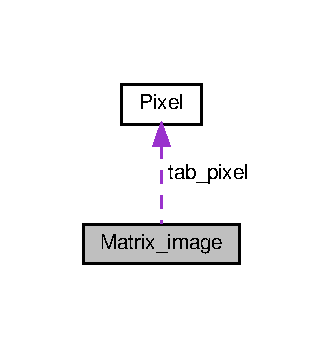
\includegraphics[width=161pt]{struct_matrix__image__coll__graph}
\end{center}
\end{figure}
\subsection*{Public Attributes}
\begin{DoxyCompactItemize}
\item 
\hyperlink{class_pixel}{Pixel} $\ast$$\ast$ \hyperlink{struct_matrix__image_a9276f0a4813f51d635278d661d5d4185}{tab\+\_\+pixel}
\item 
int \hyperlink{struct_matrix__image_ae7d959a24f238fc01c0be5a31b9ee85e}{xsize}
\item 
int \hyperlink{struct_matrix__image_acde4c9c123ca46e60af3d4a0b18d8bfd}{ysize}
\end{DoxyCompactItemize}


\subsection{Detailed Description}
~\newline
$\ast$$\ast$$\ast$$\ast$$\ast$$\ast$$\ast$$\ast$$\ast$$\ast$$\ast$$\ast$$\ast$$\ast$$\ast$$\ast$$\ast$$\ast$$\ast$$\ast$$\ast$$\ast$$\ast$$\ast$$\ast$$\ast$$\ast$$\ast$$\ast$$\ast$$\ast$$\ast$$\ast$$\ast$$\ast$$\ast$$\ast$$\ast$$\ast$$\ast$$\ast$$\ast$$\ast$$\ast$$\ast$$\ast$$\ast$$\ast$$\ast$$\ast$$\ast$$\ast$$\ast$$\ast$$\ast$$\ast$$\ast$$\ast$$\ast$$\ast$$\ast$$\ast$$\ast$$\ast$$\ast$$\ast$$\ast$$\ast$$\ast$$\ast$$\ast$$\ast$$\ast$$\ast$$\ast$$\ast$~\newline
 \textbackslash{} ~\newline
\textbackslash{} Purpose\+: ~\newline
\textbackslash{} ~\newline
\textbackslash{} Containt all pixels of the image ~\newline
\textbackslash{} ~\newline
\textbackslash{} Author\+: ~\newline
\textbackslash{} ~\newline
\textbackslash{} Stephane N\+G\+N\+E\+P\+I\+E\+P\+A\+YE W\+E\+M\+BE ~\newline
\textbackslash{} ~\newline
\textbackslash{} Parameters\+: ~\newline
\textbackslash{} ~\newline
\textbackslash{} Element1, \hyperlink{class_pixel}{Pixel} $\ast$$\ast$tab\+\_\+pixel, table of pixels. ~\newline
\textbackslash{} ~\newline
\textbackslash{} Element2, int xsize, whidth of the image (number of pixels on the whidth). ~\newline
\textbackslash{} ~\newline
\textbackslash{} Element3, int ysize, heigth of the image (number of pixels on the heigth). ~\newline
\textbackslash{} ~\newline


Definition at line 18 of file matrix\+\_\+image.\+h.



\subsection{Member Data Documentation}
\mbox{\Hypertarget{struct_matrix__image_a9276f0a4813f51d635278d661d5d4185}\label{struct_matrix__image_a9276f0a4813f51d635278d661d5d4185}} 
\index{Matrix\+\_\+image@{Matrix\+\_\+image}!tab\+\_\+pixel@{tab\+\_\+pixel}}
\index{tab\+\_\+pixel@{tab\+\_\+pixel}!Matrix\+\_\+image@{Matrix\+\_\+image}}
\subsubsection{\texorpdfstring{tab\+\_\+pixel}{tab\_pixel}}
{\footnotesize\ttfamily \hyperlink{class_pixel}{Pixel}$\ast$$\ast$ Matrix\+\_\+image\+::tab\+\_\+pixel}



Definition at line 41 of file matrix\+\_\+image.\+h.

\mbox{\Hypertarget{struct_matrix__image_ae7d959a24f238fc01c0be5a31b9ee85e}\label{struct_matrix__image_ae7d959a24f238fc01c0be5a31b9ee85e}} 
\index{Matrix\+\_\+image@{Matrix\+\_\+image}!xsize@{xsize}}
\index{xsize@{xsize}!Matrix\+\_\+image@{Matrix\+\_\+image}}
\subsubsection{\texorpdfstring{xsize}{xsize}}
{\footnotesize\ttfamily int Matrix\+\_\+image\+::xsize}



Definition at line 42 of file matrix\+\_\+image.\+h.

\mbox{\Hypertarget{struct_matrix__image_acde4c9c123ca46e60af3d4a0b18d8bfd}\label{struct_matrix__image_acde4c9c123ca46e60af3d4a0b18d8bfd}} 
\index{Matrix\+\_\+image@{Matrix\+\_\+image}!ysize@{ysize}}
\index{ysize@{ysize}!Matrix\+\_\+image@{Matrix\+\_\+image}}
\subsubsection{\texorpdfstring{ysize}{ysize}}
{\footnotesize\ttfamily int Matrix\+\_\+image\+::ysize}



Definition at line 43 of file matrix\+\_\+image.\+h.



The documentation for this struct was generated from the following file\+:\begin{DoxyCompactItemize}
\item 
/home/ngenpiepaye/\+Mon evolution/\+E\+N\+S\+T\+A/\+F\+I\+S\+E2\+A/\+C++/create\+\_\+raster/src/\hyperlink{matrix__image_8h}{matrix\+\_\+image.\+h}\end{DoxyCompactItemize}

\hypertarget{class_pixel}{}\section{Pixel Class Reference}
\label{class_pixel}\index{Pixel@{Pixel}}


{\ttfamily \#include $<$pixel.\+h$>$}

\subsection*{Public Member Functions}
\begin{DoxyCompactItemize}
\item 
\hyperlink{class_pixel_a27ad99a2f705e635c42d242d530d4756}{Pixel} ()
\item 
\hyperlink{class_pixel_a30f6aaf9a1d8792245070860546fa365}{$\sim$\+Pixel} ()
\item 
void \hyperlink{class_pixel_a0064982203ecaf79cf79ecfa04fb4f1f}{set\+\_\+val} (float val)
\item 
void \hyperlink{class_pixel_a22150f6c19217b513d58ef7ec7bda6a9}{set\+\_\+rgb\+\_\+val} ()
\end{DoxyCompactItemize}
\subsection*{Public Attributes}
\begin{DoxyCompactItemize}
\item 
float \hyperlink{class_pixel_a7deda5be756322a5c31f6c2da641fd23}{p\+\_\+f} =0
\item 
unsigned int \hyperlink{class_pixel_ab220df144b119969f66eb5fb5d75c9bb}{p\+\_\+val} = 0
\item 
unsigned int \hyperlink{class_pixel_a837be2857d4fba78615f2fb78e28e67d}{p\+\_\+r} = 0
\item 
unsigned int \hyperlink{class_pixel_ab57c1d8eb36e078122374f40101648b4}{p\+\_\+g} = 0
\item 
unsigned int \hyperlink{class_pixel_a9521bc43c95cfcb25a11b03e176ad6a1}{p\+\_\+b} = 0
\item 
int \hyperlink{class_pixel_ad6e3f83bd8d6894e3e7516a19fcef096}{p\+\_\+nb\+\_\+point} = 0
\end{DoxyCompactItemize}


\subsection{Detailed Description}
~\newline
$\ast$$\ast$$\ast$$\ast$$\ast$$\ast$$\ast$$\ast$$\ast$$\ast$$\ast$$\ast$$\ast$$\ast$$\ast$$\ast$$\ast$$\ast$$\ast$$\ast$$\ast$$\ast$$\ast$$\ast$$\ast$$\ast$$\ast$$\ast$$\ast$$\ast$$\ast$$\ast$$\ast$$\ast$$\ast$$\ast$$\ast$$\ast$$\ast$$\ast$$\ast$$\ast$$\ast$$\ast$$\ast$$\ast$$\ast$$\ast$$\ast$$\ast$$\ast$$\ast$$\ast$$\ast$$\ast$$\ast$$\ast$$\ast$$\ast$$\ast$$\ast$$\ast$$\ast$$\ast$$\ast$$\ast$$\ast$$\ast$$\ast$$\ast$$\ast$$\ast$$\ast$$\ast$$\ast$$\ast$~\newline
\textbackslash{} ~\newline
\textbackslash{} Purpose\+:~\newline
\textbackslash{} ~\newline
\textbackslash{} Class pixel, descripte the parameters of a pixel and it works~\newline
\textbackslash{} ~\newline
\textbackslash{} Author\+:~\newline
\textbackslash{} ~\newline
\textbackslash{} Stephane N\+G\+N\+E\+P\+I\+E\+P\+A\+YE W\+E\+M\+BE~\newline
\textbackslash{} ~\newline
\textbackslash{} Class variables\+:~\newline
\textbackslash{} ~\newline
\textbackslash{} Element1, unsigned int p\+\_\+val, is the value of the pixel, using for calculate gray scale color.~\newline
\textbackslash{} ~\newline
\textbackslash{} Element2, float p\+\_\+f, a number important for the calculation of R\+GB color.~\newline
\textbackslash{} ~\newline
\textbackslash{} Element3, unsigned int p\+\_\+r, p\+\_\+g, p\+\_\+b, R\+GB values for the setup of color.~\newline
\textbackslash{} ~\newline
\textbackslash{} Element4, int p\+\_\+nb\+\_\+point, number of point which contribute to the calculation of the value of the pixel, we use it for the barycenter~\newline
\textbackslash{} ~\newline


Definition at line 12 of file pixel.\+h.



\subsection{Constructor \& Destructor Documentation}
\mbox{\Hypertarget{class_pixel_a27ad99a2f705e635c42d242d530d4756}\label{class_pixel_a27ad99a2f705e635c42d242d530d4756}} 
\index{Pixel@{Pixel}!Pixel@{Pixel}}
\index{Pixel@{Pixel}!Pixel@{Pixel}}
\subsubsection{\texorpdfstring{Pixel()}{Pixel()}}
{\footnotesize\ttfamily Pixel\+::\+Pixel (\begin{DoxyParamCaption}{ }\end{DoxyParamCaption})}

~\newline
$\ast$$\ast$$\ast$$\ast$$\ast$$\ast$$\ast$$\ast$$\ast$$\ast$$\ast$$\ast$$\ast$$\ast$$\ast$$\ast$$\ast$$\ast$$\ast$$\ast$$\ast$$\ast$$\ast$$\ast$$\ast$$\ast$$\ast$$\ast$$\ast$$\ast$$\ast$$\ast$$\ast$$\ast$$\ast$$\ast$$\ast$$\ast$$\ast$$\ast$$\ast$$\ast$$\ast$$\ast$$\ast$$\ast$$\ast$$\ast$$\ast$$\ast$$\ast$$\ast$$\ast$$\ast$$\ast$$\ast$$\ast$$\ast$$\ast$$\ast$$\ast$$\ast$$\ast$$\ast$$\ast$$\ast$$\ast$$\ast$$\ast$$\ast$$\ast$$\ast$$\ast$$\ast$$\ast$$\ast$~\newline
\textbackslash{} ~\newline
\textbackslash{} Purpose\+:~\newline
\textbackslash{} ~\newline
\textbackslash{} defaut constructor of the pixel~\newline
\textbackslash{} ~\newline
\textbackslash{} Author\+:~\newline
\textbackslash{} ~\newline
\textbackslash{} stephane N\+G\+N\+E\+P\+I\+E\+P\+A\+YE W\+E\+M\+BE~\newline
\textbackslash{} ~\newline
\textbackslash{} Parameters\+:~\newline
\textbackslash{} ~\newline
\textbackslash{} No parameter~\newline
\textbackslash{} ~\newline


Definition at line 9 of file pixel.\+cpp.

\mbox{\Hypertarget{class_pixel_a30f6aaf9a1d8792245070860546fa365}\label{class_pixel_a30f6aaf9a1d8792245070860546fa365}} 
\index{Pixel@{Pixel}!````~Pixel@{$\sim$\+Pixel}}
\index{````~Pixel@{$\sim$\+Pixel}!Pixel@{Pixel}}
\subsubsection{\texorpdfstring{$\sim$\+Pixel()}{~Pixel()}}
{\footnotesize\ttfamily Pixel\+::$\sim$\+Pixel (\begin{DoxyParamCaption}{ }\end{DoxyParamCaption})}

~\newline
$\ast$$\ast$$\ast$$\ast$$\ast$$\ast$$\ast$$\ast$$\ast$$\ast$$\ast$$\ast$$\ast$$\ast$$\ast$$\ast$$\ast$$\ast$$\ast$$\ast$$\ast$$\ast$$\ast$$\ast$$\ast$$\ast$$\ast$$\ast$$\ast$$\ast$$\ast$$\ast$$\ast$$\ast$$\ast$$\ast$$\ast$$\ast$$\ast$$\ast$$\ast$$\ast$$\ast$$\ast$$\ast$$\ast$$\ast$$\ast$$\ast$$\ast$$\ast$$\ast$$\ast$$\ast$$\ast$$\ast$$\ast$$\ast$$\ast$$\ast$$\ast$$\ast$$\ast$$\ast$$\ast$$\ast$$\ast$$\ast$$\ast$$\ast$$\ast$$\ast$$\ast$$\ast$$\ast$$\ast$~\newline
\textbackslash{} ~\newline
\textbackslash{} Purpose\+:~\newline
\textbackslash{} ~\newline
\textbackslash{} desconstroctor of the pixel~\newline
\textbackslash{} ~\newline
\textbackslash{} Author\+:~\newline
\textbackslash{} ~\newline
\textbackslash{} stephane N\+G\+N\+E\+P\+I\+E\+P\+A\+YE W\+E\+M\+BE~\newline
\textbackslash{} ~\newline
\textbackslash{} Parameters\+:~\newline
\textbackslash{} ~\newline
\textbackslash{} No parameter~\newline
\textbackslash{} ~\newline


Definition at line 32 of file pixel.\+cpp.



\subsection{Member Function Documentation}
\mbox{\Hypertarget{class_pixel_a22150f6c19217b513d58ef7ec7bda6a9}\label{class_pixel_a22150f6c19217b513d58ef7ec7bda6a9}} 
\index{Pixel@{Pixel}!set\+\_\+rgb\+\_\+val@{set\+\_\+rgb\+\_\+val}}
\index{set\+\_\+rgb\+\_\+val@{set\+\_\+rgb\+\_\+val}!Pixel@{Pixel}}
\subsubsection{\texorpdfstring{set\+\_\+rgb\+\_\+val()}{set\_rgb\_val()}}
{\footnotesize\ttfamily void Pixel\+::set\+\_\+rgb\+\_\+val (\begin{DoxyParamCaption}{ }\end{DoxyParamCaption})}

~\newline
$\ast$$\ast$$\ast$$\ast$$\ast$$\ast$$\ast$$\ast$$\ast$$\ast$$\ast$$\ast$$\ast$$\ast$$\ast$$\ast$$\ast$$\ast$$\ast$$\ast$$\ast$$\ast$$\ast$$\ast$$\ast$$\ast$$\ast$$\ast$$\ast$$\ast$$\ast$$\ast$$\ast$$\ast$$\ast$$\ast$$\ast$$\ast$$\ast$$\ast$$\ast$$\ast$$\ast$$\ast$$\ast$$\ast$$\ast$$\ast$$\ast$$\ast$$\ast$$\ast$$\ast$$\ast$$\ast$$\ast$$\ast$$\ast$$\ast$$\ast$$\ast$$\ast$$\ast$$\ast$$\ast$$\ast$$\ast$$\ast$$\ast$$\ast$$\ast$$\ast$$\ast$$\ast$$\ast$$\ast$~\newline
\textbackslash{} ~\newline
\textbackslash{} Purpose\+:~\newline
\textbackslash{} ~\newline
\textbackslash{} Set the color of the pixel using \char`\"{}short rainbow R\+G\+B\char`\"{} scale for conversion~\newline
\textbackslash{} ~\newline
\textbackslash{} Author\+:~\newline
\textbackslash{} ~\newline
\textbackslash{} stephane N\+G\+N\+E\+P\+I\+E\+P\+A\+YE W\+E\+M\+BE~\newline
\textbackslash{} ~\newline
\textbackslash{} Parameters\+:~\newline
\textbackslash{} ~\newline
\textbackslash{} No parameter~\newline
\textbackslash{} ~\newline


Definition at line 82 of file pixel.\+cpp.

\mbox{\Hypertarget{class_pixel_a0064982203ecaf79cf79ecfa04fb4f1f}\label{class_pixel_a0064982203ecaf79cf79ecfa04fb4f1f}} 
\index{Pixel@{Pixel}!set\+\_\+val@{set\+\_\+val}}
\index{set\+\_\+val@{set\+\_\+val}!Pixel@{Pixel}}
\subsubsection{\texorpdfstring{set\+\_\+val()}{set\_val()}}
{\footnotesize\ttfamily void Pixel\+::set\+\_\+val (\begin{DoxyParamCaption}\item[{float}]{val }\end{DoxyParamCaption})}

~\newline
$\ast$$\ast$$\ast$$\ast$$\ast$$\ast$$\ast$$\ast$$\ast$$\ast$$\ast$$\ast$$\ast$$\ast$$\ast$$\ast$$\ast$$\ast$$\ast$$\ast$$\ast$$\ast$$\ast$$\ast$$\ast$$\ast$$\ast$$\ast$$\ast$$\ast$$\ast$$\ast$$\ast$$\ast$$\ast$$\ast$$\ast$$\ast$$\ast$$\ast$$\ast$$\ast$$\ast$$\ast$$\ast$$\ast$$\ast$$\ast$$\ast$$\ast$$\ast$$\ast$$\ast$$\ast$$\ast$$\ast$$\ast$$\ast$$\ast$$\ast$$\ast$$\ast$$\ast$$\ast$$\ast$$\ast$$\ast$$\ast$$\ast$$\ast$$\ast$$\ast$$\ast$$\ast$$\ast$$\ast$~\newline
\textbackslash{} ~\newline
\textbackslash{} Purpose\+:~\newline
\textbackslash{} ~\newline
\textbackslash{} Set the value of the pixel, this value helps for the choice of the color or the level of gray~\newline
\textbackslash{} ~\newline
\textbackslash{} Author\+:~\newline
\textbackslash{} ~\newline
\textbackslash{} stephane N\+G\+N\+E\+P\+I\+E\+P\+A\+YE W\+E\+M\+BE~\newline
\textbackslash{} ~\newline
\textbackslash{} Parameters\+:~\newline
\textbackslash{} ~\newline
\textbackslash{} Input, float val, the value of the value of the pixel depending of the altitude of the point corresponding ~\newline
\textbackslash{} ~\newline


Definition at line 56 of file pixel.\+cpp.



\subsection{Member Data Documentation}
\mbox{\Hypertarget{class_pixel_a9521bc43c95cfcb25a11b03e176ad6a1}\label{class_pixel_a9521bc43c95cfcb25a11b03e176ad6a1}} 
\index{Pixel@{Pixel}!p\+\_\+b@{p\+\_\+b}}
\index{p\+\_\+b@{p\+\_\+b}!Pixel@{Pixel}}
\subsubsection{\texorpdfstring{p\+\_\+b}{p\_b}}
{\footnotesize\ttfamily unsigned int Pixel\+::p\+\_\+b = 0}



Definition at line 45 of file pixel.\+h.

\mbox{\Hypertarget{class_pixel_a7deda5be756322a5c31f6c2da641fd23}\label{class_pixel_a7deda5be756322a5c31f6c2da641fd23}} 
\index{Pixel@{Pixel}!p\+\_\+f@{p\+\_\+f}}
\index{p\+\_\+f@{p\+\_\+f}!Pixel@{Pixel}}
\subsubsection{\texorpdfstring{p\+\_\+f}{p\_f}}
{\footnotesize\ttfamily float Pixel\+::p\+\_\+f =0}



Definition at line 43 of file pixel.\+h.

\mbox{\Hypertarget{class_pixel_ab57c1d8eb36e078122374f40101648b4}\label{class_pixel_ab57c1d8eb36e078122374f40101648b4}} 
\index{Pixel@{Pixel}!p\+\_\+g@{p\+\_\+g}}
\index{p\+\_\+g@{p\+\_\+g}!Pixel@{Pixel}}
\subsubsection{\texorpdfstring{p\+\_\+g}{p\_g}}
{\footnotesize\ttfamily unsigned int Pixel\+::p\+\_\+g = 0}



Definition at line 45 of file pixel.\+h.

\mbox{\Hypertarget{class_pixel_ad6e3f83bd8d6894e3e7516a19fcef096}\label{class_pixel_ad6e3f83bd8d6894e3e7516a19fcef096}} 
\index{Pixel@{Pixel}!p\+\_\+nb\+\_\+point@{p\+\_\+nb\+\_\+point}}
\index{p\+\_\+nb\+\_\+point@{p\+\_\+nb\+\_\+point}!Pixel@{Pixel}}
\subsubsection{\texorpdfstring{p\+\_\+nb\+\_\+point}{p\_nb\_point}}
{\footnotesize\ttfamily int Pixel\+::p\+\_\+nb\+\_\+point = 0}



Definition at line 46 of file pixel.\+h.

\mbox{\Hypertarget{class_pixel_a837be2857d4fba78615f2fb78e28e67d}\label{class_pixel_a837be2857d4fba78615f2fb78e28e67d}} 
\index{Pixel@{Pixel}!p\+\_\+r@{p\+\_\+r}}
\index{p\+\_\+r@{p\+\_\+r}!Pixel@{Pixel}}
\subsubsection{\texorpdfstring{p\+\_\+r}{p\_r}}
{\footnotesize\ttfamily unsigned int Pixel\+::p\+\_\+r = 0}



Definition at line 45 of file pixel.\+h.

\mbox{\Hypertarget{class_pixel_ab220df144b119969f66eb5fb5d75c9bb}\label{class_pixel_ab220df144b119969f66eb5fb5d75c9bb}} 
\index{Pixel@{Pixel}!p\+\_\+val@{p\+\_\+val}}
\index{p\+\_\+val@{p\+\_\+val}!Pixel@{Pixel}}
\subsubsection{\texorpdfstring{p\+\_\+val}{p\_val}}
{\footnotesize\ttfamily unsigned int Pixel\+::p\+\_\+val = 0}



Definition at line 44 of file pixel.\+h.



The documentation for this class was generated from the following files\+:\begin{DoxyCompactItemize}
\item 
/home/ngenpiepaye/\+Mon evolution/\+E\+N\+S\+T\+A/\+F\+I\+S\+E2\+A/\+C++/create\+\_\+raster/src/\hyperlink{pixel_8h}{pixel.\+h}\item 
/home/ngenpiepaye/\+Mon evolution/\+E\+N\+S\+T\+A/\+F\+I\+S\+E2\+A/\+C++/create\+\_\+raster/src/\hyperlink{pixel_8cpp}{pixel.\+cpp}\end{DoxyCompactItemize}

\hypertarget{class_point}{}\section{Point Class Reference}
\label{class_point}\index{Point@{Point}}


{\ttfamily \#include $<$point\+\_\+\+M\+N\+T.\+h$>$}

\subsection*{Public Member Functions}
\begin{DoxyCompactItemize}
\item 
\hyperlink{class_point_a11e86874da3294d7ea8b35be9cd5bd9c}{Point} (float east, float north, float level)
\item 
\hyperlink{class_point_a395fa04b4ec126b66fc053f829a30cc1}{$\sim$\+Point} ()
\end{DoxyCompactItemize}
\subsection*{Public Attributes}
\begin{DoxyCompactItemize}
\item 
float \hyperlink{class_point_a358899abd4e51fdd5322b76a8324ef90}{p\+\_\+lat}
\item 
float \hyperlink{class_point_acee2bfc413dce3e1b69524e85305980b}{p\+\_\+longi}
\item 
float \hyperlink{class_point_a7ed90ddaad8bfac738d4ac9a7b6f620f}{p\+\_\+x}
\item 
float \hyperlink{class_point_a420b83b0054d2ffc151aac30585c7f4a}{p\+\_\+y}
\item 
float \hyperlink{class_point_ae85c8ed96afee827cddee534ae367787}{p\+\_\+x\+\_\+relatif}
\item 
float \hyperlink{class_point_af5a6763229a95cb09ef94d605fe3307a}{p\+\_\+y\+\_\+relatif}
\item 
float \hyperlink{class_point_add37feb7f6e9ccb3d5ba201d82b7f7a7}{p\+\_\+i}
\item 
float \hyperlink{class_point_a53ddf5fde2dd3c2e68cf64bc6ebd6951}{p\+\_\+j}
\item 
float \hyperlink{class_point_a40457fd9b36c4414907fa67d8d99f119}{p\+\_\+level}
\end{DoxyCompactItemize}
\subsection*{Friends}
\begin{DoxyCompactItemize}
\item 
std\+::istream \& \hyperlink{class_point_af31c1932671eb01dfe5679f3c2dc6a40}{operator$>$$>$} (std\+::istream \&stream, \hyperlink{class_point}{Point} \&p)
\end{DoxyCompactItemize}


\subsection{Detailed Description}
~\newline
$\ast$$\ast$$\ast$$\ast$$\ast$$\ast$$\ast$$\ast$$\ast$$\ast$$\ast$$\ast$$\ast$$\ast$$\ast$$\ast$$\ast$$\ast$$\ast$$\ast$$\ast$$\ast$$\ast$$\ast$$\ast$$\ast$$\ast$$\ast$$\ast$$\ast$$\ast$$\ast$$\ast$$\ast$$\ast$$\ast$$\ast$$\ast$$\ast$$\ast$$\ast$$\ast$$\ast$$\ast$$\ast$$\ast$$\ast$$\ast$$\ast$$\ast$$\ast$$\ast$$\ast$$\ast$$\ast$$\ast$$\ast$$\ast$$\ast$$\ast$$\ast$$\ast$$\ast$$\ast$$\ast$$\ast$$\ast$$\ast$$\ast$$\ast$$\ast$$\ast$$\ast$$\ast$$\ast$$\ast$~\newline
\textbackslash{} ~\newline
\textbackslash{} Purpose\+:~\newline
\textbackslash{} ~\newline
\textbackslash{} Class point, descripte the parameters of a point and it works~\newline
\textbackslash{} ~\newline
\textbackslash{} Author\+:~\newline
\textbackslash{} ~\newline
\textbackslash{} Stephane N\+G\+N\+E\+P\+I\+E\+P\+A\+YE W\+E\+M\+BE~\newline
\textbackslash{} ~\newline
\textbackslash{} Class variables\+:~\newline
\textbackslash{} ~\newline
\textbackslash{} Element1, float p\+\_\+lat,p\+\_\+longi, p\+\_\+level, is the lattitude and the longitude and the level of the point.~\newline
\textbackslash{} ~\newline
\textbackslash{} Element2, float p\+\_\+x,p\+\_\+y, is the projected coordinate of the point.~\newline
\textbackslash{} ~\newline
\textbackslash{} Element3, float p\+\_\+x\+\_\+relatif, p\+\_\+y\+\_\+relatif, the relatif coordinate the point.~\newline
\textbackslash{} ~\newline
\textbackslash{} Element4, float p\+\_\+i, p\+\_\+j, is the index of the pixel associated for this point. in the image, this point will be represent by the pixel at the position p\+\_\+i, p\+\_\+j~\newline
\textbackslash{} ~\newline


Definition at line 9 of file point\+\_\+\+M\+N\+T.\+h.



\subsection{Constructor \& Destructor Documentation}
\mbox{\Hypertarget{class_point_a11e86874da3294d7ea8b35be9cd5bd9c}\label{class_point_a11e86874da3294d7ea8b35be9cd5bd9c}} 
\index{Point@{Point}!Point@{Point}}
\index{Point@{Point}!Point@{Point}}
\subsubsection{\texorpdfstring{Point()}{Point()}}
{\footnotesize\ttfamily Point\+::\+Point (\begin{DoxyParamCaption}\item[{float}]{east,  }\item[{float}]{north,  }\item[{float}]{level }\end{DoxyParamCaption})}

~\newline
$\ast$$\ast$$\ast$$\ast$$\ast$$\ast$$\ast$$\ast$$\ast$$\ast$$\ast$$\ast$$\ast$$\ast$$\ast$$\ast$$\ast$$\ast$$\ast$$\ast$$\ast$$\ast$$\ast$$\ast$$\ast$$\ast$$\ast$$\ast$$\ast$$\ast$$\ast$$\ast$$\ast$$\ast$$\ast$$\ast$$\ast$$\ast$$\ast$$\ast$$\ast$$\ast$$\ast$$\ast$$\ast$$\ast$$\ast$$\ast$$\ast$$\ast$$\ast$$\ast$$\ast$$\ast$$\ast$$\ast$$\ast$$\ast$$\ast$$\ast$$\ast$$\ast$$\ast$$\ast$$\ast$$\ast$$\ast$$\ast$$\ast$$\ast$$\ast$$\ast$$\ast$$\ast$$\ast$$\ast$~\newline
\textbackslash{} ~\newline
\textbackslash{} Purpose\+:~\newline
\textbackslash{} ~\newline
\textbackslash{} defaut constructor of a point of the M\+NT knowing the lattitude, the longitude and the level ~\newline
\textbackslash{} ~\newline
\textbackslash{} Author\+:~\newline
\textbackslash{} ~\newline
\textbackslash{} stephane N\+G\+N\+E\+P\+I\+E\+P\+A\+YE W\+E\+M\+BE~\newline
\textbackslash{} ~\newline
\textbackslash{} Parameters\+:~\newline
\textbackslash{} ~\newline
\textbackslash{} Input, float lat, the lattitude of the point~\newline
\textbackslash{} ~\newline
\textbackslash{} Input, float longi, the longitude of the point ~\newline
\textbackslash{} ~\newline
\textbackslash{} Input, float level, the altitude of the point ~\newline
\textbackslash{} ~\newline
 

Definition at line 8 of file point\+\_\+\+M\+N\+T.\+cpp.

\mbox{\Hypertarget{class_point_a395fa04b4ec126b66fc053f829a30cc1}\label{class_point_a395fa04b4ec126b66fc053f829a30cc1}} 
\index{Point@{Point}!````~Point@{$\sim$\+Point}}
\index{````~Point@{$\sim$\+Point}!Point@{Point}}
\subsubsection{\texorpdfstring{$\sim$\+Point()}{~Point()}}
{\footnotesize\ttfamily Point\+::$\sim$\+Point (\begin{DoxyParamCaption}{ }\end{DoxyParamCaption})}

~\newline
$\ast$$\ast$$\ast$$\ast$$\ast$$\ast$$\ast$$\ast$$\ast$$\ast$$\ast$$\ast$$\ast$$\ast$$\ast$$\ast$$\ast$$\ast$$\ast$$\ast$$\ast$$\ast$$\ast$$\ast$$\ast$$\ast$$\ast$$\ast$$\ast$$\ast$$\ast$$\ast$$\ast$$\ast$$\ast$$\ast$$\ast$$\ast$$\ast$$\ast$$\ast$$\ast$$\ast$$\ast$$\ast$$\ast$$\ast$$\ast$$\ast$$\ast$$\ast$$\ast$$\ast$$\ast$$\ast$$\ast$$\ast$$\ast$$\ast$$\ast$$\ast$$\ast$$\ast$$\ast$$\ast$$\ast$$\ast$$\ast$$\ast$$\ast$$\ast$$\ast$$\ast$$\ast$$\ast$$\ast$~\newline
\textbackslash{} ~\newline
\textbackslash{} Purpose\+:~\newline
\textbackslash{} ~\newline
\textbackslash{} desconstroctor of the point~\newline
\textbackslash{} ~\newline
\textbackslash{} Author\+:~\newline
\textbackslash{} ~\newline
\textbackslash{} stephane N\+G\+N\+E\+P\+I\+E\+P\+A\+YE W\+E\+M\+BE~\newline
\textbackslash{} ~\newline
\textbackslash{} Parameters\+:~\newline
\textbackslash{} ~\newline
\textbackslash{} No parameter~\newline
\textbackslash{} ~\newline
 

Definition at line 35 of file point\+\_\+\+M\+N\+T.\+cpp.



\subsection{Friends And Related Function Documentation}
\mbox{\Hypertarget{class_point_af31c1932671eb01dfe5679f3c2dc6a40}\label{class_point_af31c1932671eb01dfe5679f3c2dc6a40}} 
\index{Point@{Point}!operator$>$$>$@{operator$>$$>$}}
\index{operator$>$$>$@{operator$>$$>$}!Point@{Point}}
\subsubsection{\texorpdfstring{operator$>$$>$}{operator>>}}
{\footnotesize\ttfamily std\+::istream\& operator$>$$>$ (\begin{DoxyParamCaption}\item[{std\+::istream \&}]{stream,  }\item[{\hyperlink{class_point}{Point} \&}]{p }\end{DoxyParamCaption})\hspace{0.3cm}{\ttfamily [friend]}}

~\newline
$\ast$$\ast$$\ast$$\ast$$\ast$$\ast$$\ast$$\ast$$\ast$$\ast$$\ast$$\ast$$\ast$$\ast$$\ast$$\ast$$\ast$$\ast$$\ast$$\ast$$\ast$$\ast$$\ast$$\ast$$\ast$$\ast$$\ast$$\ast$$\ast$$\ast$$\ast$$\ast$$\ast$$\ast$$\ast$$\ast$$\ast$$\ast$$\ast$$\ast$$\ast$$\ast$$\ast$$\ast$$\ast$$\ast$$\ast$$\ast$$\ast$$\ast$$\ast$$\ast$$\ast$$\ast$$\ast$$\ast$$\ast$$\ast$$\ast$$\ast$$\ast$$\ast$$\ast$$\ast$$\ast$$\ast$$\ast$$\ast$$\ast$$\ast$$\ast$$\ast$$\ast$$\ast$$\ast$$\ast$~\newline
\textbackslash{} ~\newline
\textbackslash{} Purpose\+:~\newline
\textbackslash{} ~\newline
\textbackslash{} surcharge de l\textquotesingle{}operateur de lecture~\newline
\textbackslash{} ~\newline
\textbackslash{} Author\+:~\newline
\textbackslash{} ~\newline
\textbackslash{} stephane N\+G\+N\+E\+P\+I\+E\+P\+A\+YE W\+E\+M\+BE~\newline
\textbackslash{} ~\newline
\textbackslash{} Parameters\+:~\newline
\textbackslash{} ~\newline
\textbackslash{} Input, std\+::istream\& stream, a pointer to the file.~\newline
\textbackslash{} ~\newline
\textbackslash{} Input, \hyperlink{class_point}{Point}\& p, point which will containt the reading data.~\newline
\textbackslash{} ~\newline


Definition at line 58 of file point\+\_\+\+M\+N\+T.\+cpp.



\subsection{Member Data Documentation}
\mbox{\Hypertarget{class_point_add37feb7f6e9ccb3d5ba201d82b7f7a7}\label{class_point_add37feb7f6e9ccb3d5ba201d82b7f7a7}} 
\index{Point@{Point}!p\+\_\+i@{p\+\_\+i}}
\index{p\+\_\+i@{p\+\_\+i}!Point@{Point}}
\subsubsection{\texorpdfstring{p\+\_\+i}{p\_i}}
{\footnotesize\ttfamily float Point\+::p\+\_\+i}



Definition at line 38 of file point\+\_\+\+M\+N\+T.\+h.

\mbox{\Hypertarget{class_point_a53ddf5fde2dd3c2e68cf64bc6ebd6951}\label{class_point_a53ddf5fde2dd3c2e68cf64bc6ebd6951}} 
\index{Point@{Point}!p\+\_\+j@{p\+\_\+j}}
\index{p\+\_\+j@{p\+\_\+j}!Point@{Point}}
\subsubsection{\texorpdfstring{p\+\_\+j}{p\_j}}
{\footnotesize\ttfamily float Point\+::p\+\_\+j}



Definition at line 38 of file point\+\_\+\+M\+N\+T.\+h.

\mbox{\Hypertarget{class_point_a358899abd4e51fdd5322b76a8324ef90}\label{class_point_a358899abd4e51fdd5322b76a8324ef90}} 
\index{Point@{Point}!p\+\_\+lat@{p\+\_\+lat}}
\index{p\+\_\+lat@{p\+\_\+lat}!Point@{Point}}
\subsubsection{\texorpdfstring{p\+\_\+lat}{p\_lat}}
{\footnotesize\ttfamily float Point\+::p\+\_\+lat}



Definition at line 38 of file point\+\_\+\+M\+N\+T.\+h.

\mbox{\Hypertarget{class_point_a40457fd9b36c4414907fa67d8d99f119}\label{class_point_a40457fd9b36c4414907fa67d8d99f119}} 
\index{Point@{Point}!p\+\_\+level@{p\+\_\+level}}
\index{p\+\_\+level@{p\+\_\+level}!Point@{Point}}
\subsubsection{\texorpdfstring{p\+\_\+level}{p\_level}}
{\footnotesize\ttfamily float Point\+::p\+\_\+level}



Definition at line 38 of file point\+\_\+\+M\+N\+T.\+h.

\mbox{\Hypertarget{class_point_acee2bfc413dce3e1b69524e85305980b}\label{class_point_acee2bfc413dce3e1b69524e85305980b}} 
\index{Point@{Point}!p\+\_\+longi@{p\+\_\+longi}}
\index{p\+\_\+longi@{p\+\_\+longi}!Point@{Point}}
\subsubsection{\texorpdfstring{p\+\_\+longi}{p\_longi}}
{\footnotesize\ttfamily float Point\+::p\+\_\+longi}



Definition at line 38 of file point\+\_\+\+M\+N\+T.\+h.

\mbox{\Hypertarget{class_point_a7ed90ddaad8bfac738d4ac9a7b6f620f}\label{class_point_a7ed90ddaad8bfac738d4ac9a7b6f620f}} 
\index{Point@{Point}!p\+\_\+x@{p\+\_\+x}}
\index{p\+\_\+x@{p\+\_\+x}!Point@{Point}}
\subsubsection{\texorpdfstring{p\+\_\+x}{p\_x}}
{\footnotesize\ttfamily float Point\+::p\+\_\+x}



Definition at line 38 of file point\+\_\+\+M\+N\+T.\+h.

\mbox{\Hypertarget{class_point_ae85c8ed96afee827cddee534ae367787}\label{class_point_ae85c8ed96afee827cddee534ae367787}} 
\index{Point@{Point}!p\+\_\+x\+\_\+relatif@{p\+\_\+x\+\_\+relatif}}
\index{p\+\_\+x\+\_\+relatif@{p\+\_\+x\+\_\+relatif}!Point@{Point}}
\subsubsection{\texorpdfstring{p\+\_\+x\+\_\+relatif}{p\_x\_relatif}}
{\footnotesize\ttfamily float Point\+::p\+\_\+x\+\_\+relatif}



Definition at line 38 of file point\+\_\+\+M\+N\+T.\+h.

\mbox{\Hypertarget{class_point_a420b83b0054d2ffc151aac30585c7f4a}\label{class_point_a420b83b0054d2ffc151aac30585c7f4a}} 
\index{Point@{Point}!p\+\_\+y@{p\+\_\+y}}
\index{p\+\_\+y@{p\+\_\+y}!Point@{Point}}
\subsubsection{\texorpdfstring{p\+\_\+y}{p\_y}}
{\footnotesize\ttfamily float Point\+::p\+\_\+y}



Definition at line 38 of file point\+\_\+\+M\+N\+T.\+h.

\mbox{\Hypertarget{class_point_af5a6763229a95cb09ef94d605fe3307a}\label{class_point_af5a6763229a95cb09ef94d605fe3307a}} 
\index{Point@{Point}!p\+\_\+y\+\_\+relatif@{p\+\_\+y\+\_\+relatif}}
\index{p\+\_\+y\+\_\+relatif@{p\+\_\+y\+\_\+relatif}!Point@{Point}}
\subsubsection{\texorpdfstring{p\+\_\+y\+\_\+relatif}{p\_y\_relatif}}
{\footnotesize\ttfamily float Point\+::p\+\_\+y\+\_\+relatif}



Definition at line 38 of file point\+\_\+\+M\+N\+T.\+h.



The documentation for this class was generated from the following files\+:\begin{DoxyCompactItemize}
\item 
/home/ngenpiepaye/\+Mon evolution/\+E\+N\+S\+T\+A/\+F\+I\+S\+E2\+A/\+C++/create\+\_\+raster/src/\hyperlink{point___m_n_t_8h}{point\+\_\+\+M\+N\+T.\+h}\item 
/home/ngenpiepaye/\+Mon evolution/\+E\+N\+S\+T\+A/\+F\+I\+S\+E2\+A/\+C++/create\+\_\+raster/src/\hyperlink{point___m_n_t_8cpp}{point\+\_\+\+M\+N\+T.\+cpp}\end{DoxyCompactItemize}

\chapter{File Documentation}
\hypertarget{main_8cpp}{}\section{/home/ngenpiepaye/\+Mon evolution/\+E\+N\+S\+T\+A/\+F\+I\+S\+E2\+A/\+C++/create\+\_\+raster/src/main.cpp File Reference}
\label{main_8cpp}\index{/home/ngenpiepaye/\+Mon evolution/\+E\+N\+S\+T\+A/\+F\+I\+S\+E2\+A/\+C++/create\+\_\+raster/src/main.\+cpp@{/home/ngenpiepaye/\+Mon evolution/\+E\+N\+S\+T\+A/\+F\+I\+S\+E2\+A/\+C++/create\+\_\+raster/src/main.\+cpp}}
{\ttfamily \#include $<$cstdlib$>$}\newline
{\ttfamily \#include $<$fstream$>$}\newline
{\ttfamily \#include $<$iostream$>$}\newline
{\ttfamily \#include $<$stdio.\+h$>$}\newline
{\ttfamily \#include $<$math.\+h$>$}\newline
{\ttfamily \#include $<$vector$>$}\newline
{\ttfamily \#include $<$algorithm$>$}\newline
{\ttfamily \#include \char`\"{}proj.\+h\char`\"{}}\newline
{\ttfamily \#include \char`\"{}point\+\_\+\+M\+N\+T.\+h\char`\"{}}\newline
{\ttfamily \#include \char`\"{}matrix\+\_\+image.\+h\char`\"{}}\newline
{\ttfamily \#include \char`\"{}pgm\+\_\+io.\+h\char`\"{}}\newline
{\ttfamily \#include \char`\"{}ppm\+\_\+io.\+h\char`\"{}}\newline
Include dependency graph for main.\+cpp\+:\nopagebreak
\begin{figure}[H]
\begin{center}
\leavevmode
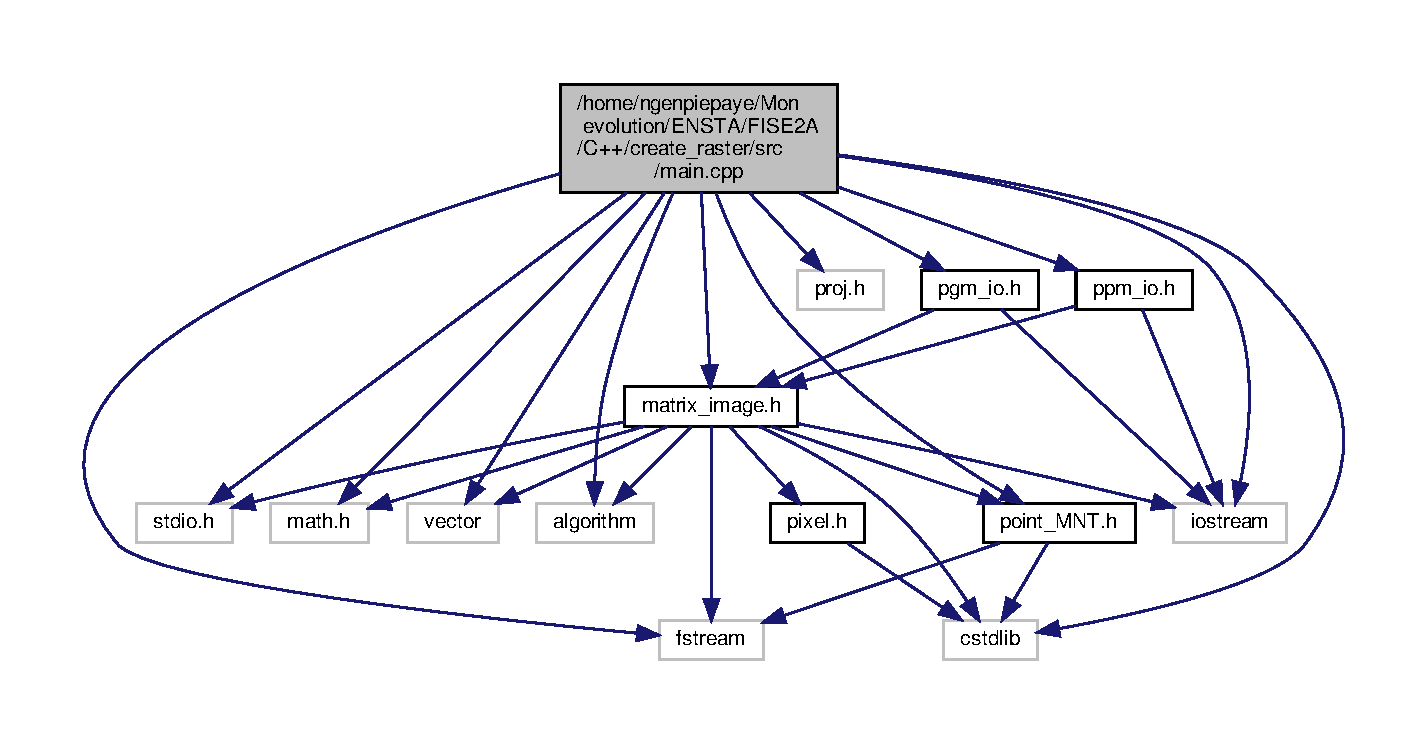
\includegraphics[width=350pt]{main_8cpp__incl}
\end{center}
\end{figure}
\subsection*{Functions}
\begin{DoxyCompactItemize}
\item 
int \hyperlink{main_8cpp_af22664d3e6f7e67e3b245504a64a0191}{projection} (vector$<$ \hyperlink{class_point}{Point} $>$ \&v\+\_\+\+Point)
\item 
void \hyperlink{main_8cpp_a5c78bfc9aa4d271163b238ae606e18b1}{setup\+\_\+relatif\+\_\+coordinate} (vector$<$ \hyperlink{class_point}{Point} $>$ \&v\+\_\+\+Point, const int \&xsize, int \&ysize)
\item 
int \hyperlink{main_8cpp_a0ddf1224851353fc92bfbff6f499fa97}{main} (int argc, char $\ast$argv\mbox{[}$\,$\mbox{]})
\end{DoxyCompactItemize}


\subsection{Function Documentation}
\mbox{\Hypertarget{main_8cpp_a0ddf1224851353fc92bfbff6f499fa97}\label{main_8cpp_a0ddf1224851353fc92bfbff6f499fa97}} 
\index{main.\+cpp@{main.\+cpp}!main@{main}}
\index{main@{main}!main.\+cpp@{main.\+cpp}}
\subsubsection{\texorpdfstring{main()}{main()}}
{\footnotesize\ttfamily int main (\begin{DoxyParamCaption}\item[{int}]{argc,  }\item[{char $\ast$}]{argv\mbox{[}$\,$\mbox{]} }\end{DoxyParamCaption})}



Definition at line 138 of file main.\+cpp.

\mbox{\Hypertarget{main_8cpp_af22664d3e6f7e67e3b245504a64a0191}\label{main_8cpp_af22664d3e6f7e67e3b245504a64a0191}} 
\index{main.\+cpp@{main.\+cpp}!projection@{projection}}
\index{projection@{projection}!main.\+cpp@{main.\+cpp}}
\subsubsection{\texorpdfstring{projection()}{projection()}}
{\footnotesize\ttfamily int projection (\begin{DoxyParamCaption}\item[{vector$<$ \hyperlink{class_point}{Point} $>$ \&}]{v\+\_\+\+Point }\end{DoxyParamCaption})}

~\newline
$\ast$$\ast$$\ast$$\ast$$\ast$$\ast$$\ast$$\ast$$\ast$$\ast$$\ast$$\ast$$\ast$$\ast$$\ast$$\ast$$\ast$$\ast$$\ast$$\ast$$\ast$$\ast$$\ast$$\ast$$\ast$$\ast$$\ast$$\ast$$\ast$$\ast$$\ast$$\ast$$\ast$$\ast$$\ast$$\ast$$\ast$$\ast$$\ast$$\ast$$\ast$$\ast$$\ast$$\ast$$\ast$$\ast$$\ast$$\ast$$\ast$$\ast$$\ast$$\ast$$\ast$$\ast$$\ast$$\ast$$\ast$$\ast$$\ast$$\ast$$\ast$$\ast$$\ast$$\ast$$\ast$$\ast$$\ast$$\ast$$\ast$$\ast$$\ast$$\ast$$\ast$$\ast$$\ast$$\ast$~\newline
\textbackslash{} ~\newline
\textbackslash{} Purpose\+:~\newline
\textbackslash{} ~\newline
\textbackslash{} Use an official projection tool (U\+T\+M30) to project all points of the M\+NT ~\newline
\textbackslash{} ~\newline
\textbackslash{} example~\newline
\textbackslash{} ~\newline
\textbackslash{} a coordinate union representing Copenhagen\+: 55d N, 12d E ~\newline
\textbackslash{} Give 285015.\+76325880236 East, 5542944.\+018361305 North in U\+T\+M30~\newline
\textbackslash{} ~\newline
\textbackslash{} Author\+:~\newline
\textbackslash{} ~\newline
\textbackslash{} Stephane N\+G\+N\+E\+P\+I\+E\+P\+A\+YE W\+E\+M\+BE~\newline
\textbackslash{} ~\newline
\textbackslash{} Parameters\+:~\newline
\textbackslash{} ~\newline
\textbackslash{} Input, vector$<$\+Point$>$\& v\+\_\+\+Point, the vector of all points of the M\+NT.~\newline
\textbackslash{} ~\newline


Definition at line 18 of file main.\+cpp.

\mbox{\Hypertarget{main_8cpp_a5c78bfc9aa4d271163b238ae606e18b1}\label{main_8cpp_a5c78bfc9aa4d271163b238ae606e18b1}} 
\index{main.\+cpp@{main.\+cpp}!setup\+\_\+relatif\+\_\+coordinate@{setup\+\_\+relatif\+\_\+coordinate}}
\index{setup\+\_\+relatif\+\_\+coordinate@{setup\+\_\+relatif\+\_\+coordinate}!main.\+cpp@{main.\+cpp}}
\subsubsection{\texorpdfstring{setup\+\_\+relatif\+\_\+coordinate()}{setup\_relatif\_coordinate()}}
{\footnotesize\ttfamily void setup\+\_\+relatif\+\_\+coordinate (\begin{DoxyParamCaption}\item[{vector$<$ \hyperlink{class_point}{Point} $>$ \&}]{v\+\_\+\+Point,  }\item[{const int \&}]{xsize,  }\item[{int \&}]{ysize }\end{DoxyParamCaption})}

~\newline
$\ast$$\ast$$\ast$$\ast$$\ast$$\ast$$\ast$$\ast$$\ast$$\ast$$\ast$$\ast$$\ast$$\ast$$\ast$$\ast$$\ast$$\ast$$\ast$$\ast$$\ast$$\ast$$\ast$$\ast$$\ast$$\ast$$\ast$$\ast$$\ast$$\ast$$\ast$$\ast$$\ast$$\ast$$\ast$$\ast$$\ast$$\ast$$\ast$$\ast$$\ast$$\ast$$\ast$$\ast$$\ast$$\ast$$\ast$$\ast$$\ast$$\ast$$\ast$$\ast$$\ast$$\ast$$\ast$$\ast$$\ast$$\ast$$\ast$$\ast$$\ast$$\ast$$\ast$$\ast$$\ast$$\ast$$\ast$$\ast$$\ast$$\ast$$\ast$$\ast$$\ast$$\ast$$\ast$$\ast$ ~\newline
\textbackslash{} ~\newline
\textbackslash{} Purpose\+: ~\newline
\textbackslash{} ~\newline
\textbackslash{} Set up relatifs coordinates of all points. whe search the minimal square which containt all points ~\newline
\textbackslash{} In the same time we calculate numbers of pixels (width, height) that we will use to represent the image, ~\newline
\textbackslash{} ~\newline
\textbackslash{} we know the whith = xsize ==$>$ resolution = xsize/amplitude\+\_\+of\+\_\+x ~\newline
\textbackslash{} we find height = ysize = resolution $\ast$ amplitude\+\_\+of\+\_\+y ~\newline
\textbackslash{} ~\newline
\textbackslash{} Author\+: ~\newline
\textbackslash{} ~\newline
\textbackslash{} Stephane N\+G\+N\+E\+P\+I\+E\+P\+A\+YE W\+E\+M\+BE ~\newline
\textbackslash{} ~\newline
\textbackslash{} Parameters\+: ~\newline
\textbackslash{} ~\newline
\textbackslash{} Input, vector$<$\+Point$>$\& v\+\_\+\+Point, the vector of all points of the M\+NT. ~\newline
\textbackslash{} Input, const int\& xsize, the whith of the image ~\newline
\textbackslash{} Input, int\& ysize, the height of the image ~\newline
\textbackslash{} ~\newline


Definition at line 88 of file main.\+cpp.


\hypertarget{matrix__image_8cpp}{}\section{/home/ngenpiepaye/\+Mon evolution/\+E\+N\+S\+T\+A/\+F\+I\+S\+E2\+A/\+C++/create\+\_\+raster/src/matrix\+\_\+image.cpp File Reference}
\label{matrix__image_8cpp}\index{/home/ngenpiepaye/\+Mon evolution/\+E\+N\+S\+T\+A/\+F\+I\+S\+E2\+A/\+C++/create\+\_\+raster/src/matrix\+\_\+image.\+cpp@{/home/ngenpiepaye/\+Mon evolution/\+E\+N\+S\+T\+A/\+F\+I\+S\+E2\+A/\+C++/create\+\_\+raster/src/matrix\+\_\+image.\+cpp}}
{\ttfamily \#include $<$cstdlib$>$}\newline
{\ttfamily \#include $<$fstream$>$}\newline
{\ttfamily \#include $<$iostream$>$}\newline
{\ttfamily \#include $<$stdio.\+h$>$}\newline
{\ttfamily \#include $<$cmath$>$}\newline
{\ttfamily \#include $<$vector$>$}\newline
{\ttfamily \#include $<$algorithm$>$}\newline
{\ttfamily \#include \char`\"{}matrix\+\_\+image.\+h\char`\"{}}\newline
{\ttfamily \#include \char`\"{}point\+\_\+\+M\+N\+T.\+h\char`\"{}}\newline
{\ttfamily \#include \char`\"{}pixel.\+h\char`\"{}}\newline
Include dependency graph for matrix\+\_\+image.\+cpp\+:\nopagebreak
\begin{figure}[H]
\begin{center}
\leavevmode
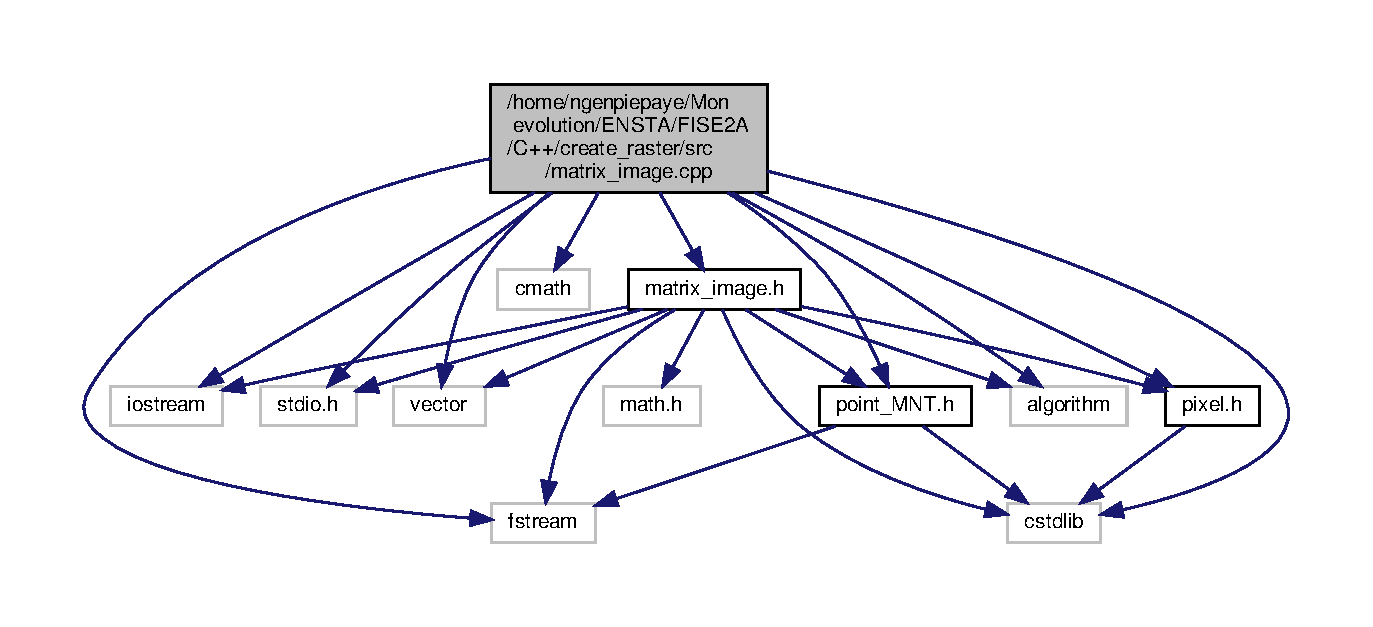
\includegraphics[width=350pt]{matrix__image_8cpp__incl}
\end{center}
\end{figure}
\subsection*{Functions}
\begin{DoxyCompactItemize}
\item 
bool \hyperlink{matrix__image_8cpp_a621c37d96a7309382336d7efe143ff14}{compx} (const \hyperlink{class_point}{Point} \&p1, const \hyperlink{class_point}{Point} \&p2)
\item 
bool \hyperlink{matrix__image_8cpp_a10418f2e697e64aa06d030e2c6380464}{compy} (const \hyperlink{class_point}{Point} \&p1, const \hyperlink{class_point}{Point} \&p2)
\item 
bool \hyperlink{matrix__image_8cpp_a4de98c177b2c83ccf77dbb1cc2e266a7}{compz} (const \hyperlink{class_point}{Point} \&p1, const \hyperlink{class_point}{Point} \&p2)
\item 
void \hyperlink{matrix__image_8cpp_a1248e095df9c969f43fe954f9030236b}{readdata} (const string \&file\+\_\+name, vector$<$ \hyperlink{class_point}{Point} $>$ \&v\+\_\+\+Point)
\item 
void \hyperlink{matrix__image_8cpp_a25661ba2304c5f5ac7dd0faee662490a}{init\+\_\+\+Matrix\+\_\+image} (\hyperlink{struct_matrix__image}{Matrix\+\_\+image} \&matrix, int xsize, int ysize)
\item 
void \hyperlink{matrix__image_8cpp_a7ec590a2c385199d60e2e2f745b47193}{setup\+\_\+index\+\_\+pixel} (vector$<$ \hyperlink{class_point}{Point} $>$ \&v\+\_\+\+Point, \hyperlink{struct_matrix__image}{Matrix\+\_\+image} \&matrix)
\item 
void \hyperlink{matrix__image_8cpp_a6260293731b54842c441b7d643433469}{setup\+\_\+value\+\_\+pixel} (\hyperlink{struct_matrix__image}{Matrix\+\_\+image} \&matrix, vector$<$ \hyperlink{class_point}{Point} $>$ \&v\+\_\+\+Point)
\item 
void \hyperlink{matrix__image_8cpp_a8edbd41f8186f1314ce9b89466daa6a7}{set\+\_\+shadow} (\hyperlink{struct_matrix__image}{Matrix\+\_\+image} \&matrix, float Altitude, float Azimuth, float cellsize)
\end{DoxyCompactItemize}


\subsection{Function Documentation}
\mbox{\Hypertarget{matrix__image_8cpp_a621c37d96a7309382336d7efe143ff14}\label{matrix__image_8cpp_a621c37d96a7309382336d7efe143ff14}} 
\index{matrix\+\_\+image.\+cpp@{matrix\+\_\+image.\+cpp}!compx@{compx}}
\index{compx@{compx}!matrix\+\_\+image.\+cpp@{matrix\+\_\+image.\+cpp}}
\subsubsection{\texorpdfstring{compx()}{compx()}}
{\footnotesize\ttfamily bool compx (\begin{DoxyParamCaption}\item[{const \hyperlink{class_point}{Point} \&}]{p1,  }\item[{const \hyperlink{class_point}{Point} \&}]{p2 }\end{DoxyParamCaption})}

~\newline
$\ast$$\ast$$\ast$$\ast$$\ast$$\ast$$\ast$$\ast$$\ast$$\ast$$\ast$$\ast$$\ast$$\ast$$\ast$$\ast$$\ast$$\ast$$\ast$$\ast$$\ast$$\ast$$\ast$$\ast$$\ast$$\ast$$\ast$$\ast$$\ast$$\ast$$\ast$$\ast$$\ast$$\ast$$\ast$$\ast$$\ast$$\ast$$\ast$$\ast$$\ast$$\ast$$\ast$$\ast$$\ast$$\ast$$\ast$$\ast$$\ast$$\ast$$\ast$$\ast$$\ast$$\ast$$\ast$$\ast$$\ast$$\ast$$\ast$$\ast$$\ast$$\ast$$\ast$$\ast$$\ast$$\ast$$\ast$$\ast$$\ast$$\ast$$\ast$$\ast$$\ast$$\ast$$\ast$$\ast$ ~\newline
\textbackslash{} ~\newline
\textbackslash{} Purpose\+: ~\newline
\textbackslash{} ~\newline
\textbackslash{} Compare two points using the x coordinate of points ~\newline
\textbackslash{} ~\newline
\textbackslash{} example ~\newline
\textbackslash{} ~\newline
\textbackslash{} P1(5, 2, 8) , P2(3, 7, 4) ==$>$ P1 $>$ P2 ~\newline
\textbackslash{} ~\newline
\textbackslash{} Author\+: ~\newline
\textbackslash{} ~\newline
\textbackslash{} Stephane N\+G\+N\+E\+P\+I\+E\+P\+A\+YE W\+E\+M\+BE ~\newline
\textbackslash{} ~\newline
\textbackslash{} Parameters\+: ~\newline
\textbackslash{} ~\newline
\textbackslash{} Input, const \hyperlink{class_point}{Point}\& p1, the first point to compare. ~\newline
\textbackslash{} ~\newline
\textbackslash{} Input, const \hyperlink{class_point}{Point}\& p2, the second point to compare. ~\newline
\textbackslash{} ~\newline


Definition at line 15 of file matrix\+\_\+image.\+cpp.

\mbox{\Hypertarget{matrix__image_8cpp_a10418f2e697e64aa06d030e2c6380464}\label{matrix__image_8cpp_a10418f2e697e64aa06d030e2c6380464}} 
\index{matrix\+\_\+image.\+cpp@{matrix\+\_\+image.\+cpp}!compy@{compy}}
\index{compy@{compy}!matrix\+\_\+image.\+cpp@{matrix\+\_\+image.\+cpp}}
\subsubsection{\texorpdfstring{compy()}{compy()}}
{\footnotesize\ttfamily bool compy (\begin{DoxyParamCaption}\item[{const \hyperlink{class_point}{Point} \&}]{p1,  }\item[{const \hyperlink{class_point}{Point} \&}]{p2 }\end{DoxyParamCaption})}

~\newline
$\ast$$\ast$$\ast$$\ast$$\ast$$\ast$$\ast$$\ast$$\ast$$\ast$$\ast$$\ast$$\ast$$\ast$$\ast$$\ast$$\ast$$\ast$$\ast$$\ast$$\ast$$\ast$$\ast$$\ast$$\ast$$\ast$$\ast$$\ast$$\ast$$\ast$$\ast$$\ast$$\ast$$\ast$$\ast$$\ast$$\ast$$\ast$$\ast$$\ast$$\ast$$\ast$$\ast$$\ast$$\ast$$\ast$$\ast$$\ast$$\ast$$\ast$$\ast$$\ast$$\ast$$\ast$$\ast$$\ast$$\ast$$\ast$$\ast$$\ast$$\ast$$\ast$$\ast$$\ast$$\ast$$\ast$$\ast$$\ast$$\ast$$\ast$$\ast$$\ast$$\ast$$\ast$$\ast$$\ast$ ~\newline
\textbackslash{} ~\newline
\textbackslash{} Purpose\+: ~\newline
\textbackslash{} ~\newline
\textbackslash{} Compare two points using the y coordinate of points ~\newline
\textbackslash{} ~\newline
\textbackslash{} example ~\newline
\textbackslash{} ~\newline
\textbackslash{} P1(5, 2, 8) , P2(3, 7, 4) ==$>$ P2 $>$ P1 ~\newline
\textbackslash{} ~\newline
\textbackslash{} Author\+: ~\newline
\textbackslash{} ~\newline
\textbackslash{} Stephane N\+G\+N\+E\+P\+I\+E\+P\+A\+YE W\+E\+M\+BE ~\newline
\textbackslash{} ~\newline
\textbackslash{} Parameters\+: ~\newline
\textbackslash{} ~\newline
\textbackslash{} Input, const \hyperlink{class_point}{Point}\& p1, the first point to compare. ~\newline
\textbackslash{} ~\newline
\textbackslash{} Input, const \hyperlink{class_point}{Point}\& p2, the second point to compare. ~\newline
\textbackslash{} ~\newline


Definition at line 45 of file matrix\+\_\+image.\+cpp.

\mbox{\Hypertarget{matrix__image_8cpp_a4de98c177b2c83ccf77dbb1cc2e266a7}\label{matrix__image_8cpp_a4de98c177b2c83ccf77dbb1cc2e266a7}} 
\index{matrix\+\_\+image.\+cpp@{matrix\+\_\+image.\+cpp}!compz@{compz}}
\index{compz@{compz}!matrix\+\_\+image.\+cpp@{matrix\+\_\+image.\+cpp}}
\subsubsection{\texorpdfstring{compz()}{compz()}}
{\footnotesize\ttfamily bool compz (\begin{DoxyParamCaption}\item[{const \hyperlink{class_point}{Point} \&}]{p1,  }\item[{const \hyperlink{class_point}{Point} \&}]{p2 }\end{DoxyParamCaption})}

~\newline
$\ast$$\ast$$\ast$$\ast$$\ast$$\ast$$\ast$$\ast$$\ast$$\ast$$\ast$$\ast$$\ast$$\ast$$\ast$$\ast$$\ast$$\ast$$\ast$$\ast$$\ast$$\ast$$\ast$$\ast$$\ast$$\ast$$\ast$$\ast$$\ast$$\ast$$\ast$$\ast$$\ast$$\ast$$\ast$$\ast$$\ast$$\ast$$\ast$$\ast$$\ast$$\ast$$\ast$$\ast$$\ast$$\ast$$\ast$$\ast$$\ast$$\ast$$\ast$$\ast$$\ast$$\ast$$\ast$$\ast$$\ast$$\ast$$\ast$$\ast$$\ast$$\ast$$\ast$$\ast$$\ast$$\ast$$\ast$$\ast$$\ast$$\ast$$\ast$$\ast$$\ast$$\ast$$\ast$$\ast$ ~\newline
\textbackslash{} ~\newline
\textbackslash{} Purpose\+: ~\newline
\textbackslash{} ~\newline
\textbackslash{} Compare two points using the z coordinate of points ~\newline
\textbackslash{} ~\newline
\textbackslash{} example ~\newline
\textbackslash{} ~\newline
\textbackslash{} P1(5, 2, 8) , P2(3, 7, 4) ==$>$ P1 $>$ P2 ~\newline
\textbackslash{} ~\newline
\textbackslash{} Author\+: ~\newline
\textbackslash{} ~\newline
\textbackslash{} Stephane N\+G\+N\+E\+P\+I\+E\+P\+A\+YE W\+E\+M\+BE ~\newline
\textbackslash{} ~\newline
\textbackslash{} Parameters\+: ~\newline
\textbackslash{} ~\newline
\textbackslash{} Input, const \hyperlink{class_point}{Point}\& p1, the first point to compare. ~\newline
\textbackslash{} ~\newline
\textbackslash{} Input, const \hyperlink{class_point}{Point}\& p2, the second point to compare. ~\newline
\textbackslash{} ~\newline


Definition at line 75 of file matrix\+\_\+image.\+cpp.

\mbox{\Hypertarget{matrix__image_8cpp_a25661ba2304c5f5ac7dd0faee662490a}\label{matrix__image_8cpp_a25661ba2304c5f5ac7dd0faee662490a}} 
\index{matrix\+\_\+image.\+cpp@{matrix\+\_\+image.\+cpp}!init\+\_\+\+Matrix\+\_\+image@{init\+\_\+\+Matrix\+\_\+image}}
\index{init\+\_\+\+Matrix\+\_\+image@{init\+\_\+\+Matrix\+\_\+image}!matrix\+\_\+image.\+cpp@{matrix\+\_\+image.\+cpp}}
\subsubsection{\texorpdfstring{init\+\_\+\+Matrix\+\_\+image()}{init\_Matrix\_image()}}
{\footnotesize\ttfamily void init\+\_\+\+Matrix\+\_\+image (\begin{DoxyParamCaption}\item[{\hyperlink{struct_matrix__image}{Matrix\+\_\+image} \&}]{matrix,  }\item[{int}]{xsize,  }\item[{int}]{ysize }\end{DoxyParamCaption})}

~\newline
$\ast$$\ast$$\ast$$\ast$$\ast$$\ast$$\ast$$\ast$$\ast$$\ast$$\ast$$\ast$$\ast$$\ast$$\ast$$\ast$$\ast$$\ast$$\ast$$\ast$$\ast$$\ast$$\ast$$\ast$$\ast$$\ast$$\ast$$\ast$$\ast$$\ast$$\ast$$\ast$$\ast$$\ast$$\ast$$\ast$$\ast$$\ast$$\ast$$\ast$$\ast$$\ast$$\ast$$\ast$$\ast$$\ast$$\ast$$\ast$$\ast$$\ast$$\ast$$\ast$$\ast$$\ast$$\ast$$\ast$$\ast$$\ast$$\ast$$\ast$$\ast$$\ast$$\ast$$\ast$$\ast$$\ast$$\ast$$\ast$$\ast$$\ast$$\ast$$\ast$$\ast$$\ast$$\ast$$\ast$ ~\newline
\textbackslash{} ~\newline
\textbackslash{} Purpose\+:~\newline
\textbackslash{} ~\newline
\textbackslash{} Create a matrix of pixel and initialize these pixels ~\newline
\textbackslash{} ~\newline
\textbackslash{} Author\+: ~\newline
\textbackslash{} ~\newline
\textbackslash{} Stephane N\+G\+N\+E\+P\+I\+E\+P\+A\+YE W\+E\+M\+BE ~\newline
\textbackslash{} ~\newline
\textbackslash{} Parameters\+: ~\newline
\textbackslash{} ~\newline
\textbackslash{} Input, \hyperlink{struct_matrix__image}{Matrix\+\_\+image}\& matrix, matrix of pixels of the image ~\newline
\textbackslash{} Input, const int\& xsize, the whith of the image (number of pixels on the whidth) ~\newline
\textbackslash{} Input, int\& ysize, the height of the image (number of pixels on the heigth) ~\newline
\textbackslash{} ~\newline


Definition at line 160 of file matrix\+\_\+image.\+cpp.

\mbox{\Hypertarget{matrix__image_8cpp_a1248e095df9c969f43fe954f9030236b}\label{matrix__image_8cpp_a1248e095df9c969f43fe954f9030236b}} 
\index{matrix\+\_\+image.\+cpp@{matrix\+\_\+image.\+cpp}!readdata@{readdata}}
\index{readdata@{readdata}!matrix\+\_\+image.\+cpp@{matrix\+\_\+image.\+cpp}}
\subsubsection{\texorpdfstring{readdata()}{readdata()}}
{\footnotesize\ttfamily void readdata (\begin{DoxyParamCaption}\item[{const string \&}]{file\+\_\+name,  }\item[{vector$<$ \hyperlink{class_point}{Point} $>$ \&}]{v\+\_\+\+Point }\end{DoxyParamCaption})}

~\newline
$\ast$$\ast$$\ast$$\ast$$\ast$$\ast$$\ast$$\ast$$\ast$$\ast$$\ast$$\ast$$\ast$$\ast$$\ast$$\ast$$\ast$$\ast$$\ast$$\ast$$\ast$$\ast$$\ast$$\ast$$\ast$$\ast$$\ast$$\ast$$\ast$$\ast$$\ast$$\ast$$\ast$$\ast$$\ast$$\ast$$\ast$$\ast$$\ast$$\ast$$\ast$$\ast$$\ast$$\ast$$\ast$$\ast$$\ast$$\ast$$\ast$$\ast$$\ast$$\ast$$\ast$$\ast$$\ast$$\ast$$\ast$$\ast$$\ast$$\ast$$\ast$$\ast$$\ast$$\ast$$\ast$$\ast$$\ast$$\ast$$\ast$$\ast$$\ast$$\ast$$\ast$$\ast$$\ast$$\ast$$\ast$ ~\newline
\textbackslash{} ~\newline
\textbackslash{} Purpose\+: ~\newline
\textbackslash{} ~\newline
\textbackslash{} Extract data of the M\+NT and put them inside a vector ~\newline
\textbackslash{} ~\newline
\textbackslash{} example ~\newline
\textbackslash{} ~\newline
\textbackslash{} 48.\+19517461 -\/3.\+028930672 -\/117.\+281 ~\newline
\textbackslash{} 48.\+19517496 -\/3.\+028923963 -\/117.\+469 ~\newline
\textbackslash{} 48.\+1951753 -\/3.\+028917253 -\/117.\+527 ~\newline
\textbackslash{} 48.\+19517564 -\/3.\+028910544 -\/117.\+506 ~\newline
\textbackslash{} 48.\+19517738 -\/3.\+028964733 -\/116.\+976 ~\newline
\textbackslash{} ..... ~\newline
\textbackslash{} ~\newline
\textbackslash{} Author\+: ~\newline
\textbackslash{} ~\newline
\textbackslash{} Stephane N\+G\+N\+E\+P\+I\+E\+P\+A\+YE W\+E\+M\+BE ~\newline
\textbackslash{} ~\newline
\textbackslash{} Parameters\+: ~\newline
\textbackslash{} ~\newline
\textbackslash{} Input, const string\& file\+\_\+name, the name of the file containing data to extract. ~\newline
\textbackslash{} ~\newline
\textbackslash{} Input, vector$<$\+Point$>$\& v\+\_\+\+Point, the vector to fill. ~\newline
\textbackslash{} ~\newline


Definition at line 105 of file matrix\+\_\+image.\+cpp.

\mbox{\Hypertarget{matrix__image_8cpp_a8edbd41f8186f1314ce9b89466daa6a7}\label{matrix__image_8cpp_a8edbd41f8186f1314ce9b89466daa6a7}} 
\index{matrix\+\_\+image.\+cpp@{matrix\+\_\+image.\+cpp}!set\+\_\+shadow@{set\+\_\+shadow}}
\index{set\+\_\+shadow@{set\+\_\+shadow}!matrix\+\_\+image.\+cpp@{matrix\+\_\+image.\+cpp}}
\subsubsection{\texorpdfstring{set\+\_\+shadow()}{set\_shadow()}}
{\footnotesize\ttfamily void set\+\_\+shadow (\begin{DoxyParamCaption}\item[{\hyperlink{struct_matrix__image}{Matrix\+\_\+image} \&}]{matrix,  }\item[{float}]{Altitude,  }\item[{float}]{Azimuth,  }\item[{float}]{cellsize }\end{DoxyParamCaption})}

~\newline
$\ast$$\ast$$\ast$$\ast$$\ast$$\ast$$\ast$$\ast$$\ast$$\ast$$\ast$$\ast$$\ast$$\ast$$\ast$$\ast$$\ast$$\ast$$\ast$$\ast$$\ast$$\ast$$\ast$$\ast$$\ast$$\ast$$\ast$$\ast$$\ast$$\ast$$\ast$$\ast$$\ast$$\ast$$\ast$$\ast$$\ast$$\ast$$\ast$$\ast$$\ast$$\ast$$\ast$$\ast$$\ast$$\ast$$\ast$$\ast$$\ast$$\ast$$\ast$$\ast$$\ast$$\ast$$\ast$$\ast$$\ast$$\ast$$\ast$$\ast$$\ast$$\ast$$\ast$$\ast$$\ast$$\ast$$\ast$$\ast$$\ast$$\ast$$\ast$$\ast$$\ast$$\ast$$\ast$$\ast$ ~\newline
\textbackslash{} ~\newline
\textbackslash{} Purpose\+:~\newline
\textbackslash{} ~\newline
\textbackslash{} mise de l\textquotesingle{}ombrage mais ne fonctionne pas encore ~\newline
\textbackslash{} ~\newline
\textbackslash{} Author\+:~\newline
\textbackslash{} ~\newline
\textbackslash{} Stephane N\+G\+N\+E\+P\+I\+E\+P\+A\+YE W\+E\+M\+BE ~\newline
\textbackslash{} ~\newline
\textbackslash{} Parameters\+: ~\newline
\textbackslash{} ~\newline
\textbackslash{} Input, \hyperlink{struct_matrix__image}{Matrix\+\_\+image}\& matrix, matrix of pixels of the image ~\newline
\textbackslash{} ~\newline


Definition at line 309 of file matrix\+\_\+image.\+cpp.

\mbox{\Hypertarget{matrix__image_8cpp_a7ec590a2c385199d60e2e2f745b47193}\label{matrix__image_8cpp_a7ec590a2c385199d60e2e2f745b47193}} 
\index{matrix\+\_\+image.\+cpp@{matrix\+\_\+image.\+cpp}!setup\+\_\+index\+\_\+pixel@{setup\+\_\+index\+\_\+pixel}}
\index{setup\+\_\+index\+\_\+pixel@{setup\+\_\+index\+\_\+pixel}!matrix\+\_\+image.\+cpp@{matrix\+\_\+image.\+cpp}}
\subsubsection{\texorpdfstring{setup\+\_\+index\+\_\+pixel()}{setup\_index\_pixel()}}
{\footnotesize\ttfamily void setup\+\_\+index\+\_\+pixel (\begin{DoxyParamCaption}\item[{vector$<$ \hyperlink{class_point}{Point} $>$ \&}]{v\+\_\+\+Point,  }\item[{\hyperlink{struct_matrix__image}{Matrix\+\_\+image} \&}]{matrix }\end{DoxyParamCaption})}

~\newline
$\ast$$\ast$$\ast$$\ast$$\ast$$\ast$$\ast$$\ast$$\ast$$\ast$$\ast$$\ast$$\ast$$\ast$$\ast$$\ast$$\ast$$\ast$$\ast$$\ast$$\ast$$\ast$$\ast$$\ast$$\ast$$\ast$$\ast$$\ast$$\ast$$\ast$$\ast$$\ast$$\ast$$\ast$$\ast$$\ast$$\ast$$\ast$$\ast$$\ast$$\ast$$\ast$$\ast$$\ast$$\ast$$\ast$$\ast$$\ast$$\ast$$\ast$$\ast$$\ast$$\ast$$\ast$$\ast$$\ast$$\ast$$\ast$$\ast$$\ast$$\ast$$\ast$$\ast$$\ast$$\ast$$\ast$$\ast$$\ast$$\ast$$\ast$$\ast$$\ast$$\ast$$\ast$$\ast$$\ast$ ~\newline
\textbackslash{} ~\newline
\textbackslash{} Purpose\+: ~\newline
\textbackslash{} ~\newline
\textbackslash{} Set up of index of pixel inside the pixel matrix of the image ~\newline
\textbackslash{} for each element of list of point of the M\+NT we find which pixel corresponding to that point ~\newline
\textbackslash{} ~\newline
\textbackslash{} Author\+:~\newline
\textbackslash{} ~\newline
\textbackslash{} Stephane N\+G\+N\+E\+P\+I\+E\+P\+A\+YE W\+E\+M\+BE ~\newline
\textbackslash{} ~\newline
\textbackslash{} Parameters\+: ~\newline
\textbackslash{} ~\newline
\textbackslash{} Input, vector$<$\+Point$>$\& v\+\_\+\+Point, the vector of all points of the M\+NT. ~\newline
\textbackslash{} Input, \hyperlink{struct_matrix__image}{Matrix\+\_\+image}\& matrix, the matrix which containt all pixel of the image to set up ~\newline
\textbackslash{} ~\newline


Definition at line 202 of file matrix\+\_\+image.\+cpp.

\mbox{\Hypertarget{matrix__image_8cpp_a6260293731b54842c441b7d643433469}\label{matrix__image_8cpp_a6260293731b54842c441b7d643433469}} 
\index{matrix\+\_\+image.\+cpp@{matrix\+\_\+image.\+cpp}!setup\+\_\+value\+\_\+pixel@{setup\+\_\+value\+\_\+pixel}}
\index{setup\+\_\+value\+\_\+pixel@{setup\+\_\+value\+\_\+pixel}!matrix\+\_\+image.\+cpp@{matrix\+\_\+image.\+cpp}}
\subsubsection{\texorpdfstring{setup\+\_\+value\+\_\+pixel()}{setup\_value\_pixel()}}
{\footnotesize\ttfamily void setup\+\_\+value\+\_\+pixel (\begin{DoxyParamCaption}\item[{\hyperlink{struct_matrix__image}{Matrix\+\_\+image} \&}]{matrix,  }\item[{vector$<$ \hyperlink{class_point}{Point} $>$ \&}]{v\+\_\+\+Point }\end{DoxyParamCaption})}

~\newline
$\ast$$\ast$$\ast$$\ast$$\ast$$\ast$$\ast$$\ast$$\ast$$\ast$$\ast$$\ast$$\ast$$\ast$$\ast$$\ast$$\ast$$\ast$$\ast$$\ast$$\ast$$\ast$$\ast$$\ast$$\ast$$\ast$$\ast$$\ast$$\ast$$\ast$$\ast$$\ast$$\ast$$\ast$$\ast$$\ast$$\ast$$\ast$$\ast$$\ast$$\ast$$\ast$$\ast$$\ast$$\ast$$\ast$$\ast$$\ast$$\ast$$\ast$$\ast$$\ast$$\ast$$\ast$$\ast$$\ast$$\ast$$\ast$$\ast$$\ast$$\ast$$\ast$$\ast$$\ast$$\ast$$\ast$$\ast$$\ast$$\ast$$\ast$$\ast$$\ast$$\ast$$\ast$$\ast$$\ast$ ~\newline
\textbackslash{} ~\newline
\textbackslash{} Purpose\+: ~\newline
\textbackslash{} ~\newline
\textbackslash{} Set up of the value of pixel inside the pixel matrix of the image ~\newline
\textbackslash{} ~\newline
\textbackslash{} Author\+:~\newline
\textbackslash{} ~\newline
\textbackslash{} Stephane N\+G\+N\+E\+P\+I\+E\+P\+A\+YE W\+E\+M\+BE ~\newline
\textbackslash{} ~\newline
\textbackslash{} Parameters\+:~\newline
\textbackslash{} ~\newline
\textbackslash{} Input, vector$<$\+Point$>$\& v\+\_\+\+Point, the vector of all points of the M\+NT.~\newline
\textbackslash{} Input, \hyperlink{struct_matrix__image}{Matrix\+\_\+image}\& matrix, the matrix which containt all pixel of the image to set up~\newline
\textbackslash{} ~\newline


Definition at line 252 of file matrix\+\_\+image.\+cpp.


\hypertarget{matrix__image_8h}{}\section{/home/ngenpiepaye/\+Mon evolution/\+E\+N\+S\+T\+A/\+F\+I\+S\+E2\+A/\+C++/create\+\_\+raster/src/matrix\+\_\+image.h File Reference}
\label{matrix__image_8h}\index{/home/ngenpiepaye/\+Mon evolution/\+E\+N\+S\+T\+A/\+F\+I\+S\+E2\+A/\+C++/create\+\_\+raster/src/matrix\+\_\+image.\+h@{/home/ngenpiepaye/\+Mon evolution/\+E\+N\+S\+T\+A/\+F\+I\+S\+E2\+A/\+C++/create\+\_\+raster/src/matrix\+\_\+image.\+h}}
{\ttfamily \#include $<$cstdlib$>$}\newline
{\ttfamily \#include $<$fstream$>$}\newline
{\ttfamily \#include $<$iostream$>$}\newline
{\ttfamily \#include $<$stdio.\+h$>$}\newline
{\ttfamily \#include $<$math.\+h$>$}\newline
{\ttfamily \#include $<$vector$>$}\newline
{\ttfamily \#include $<$algorithm$>$}\newline
{\ttfamily \#include \char`\"{}point\+\_\+\+M\+N\+T.\+h\char`\"{}}\newline
{\ttfamily \#include \char`\"{}pixel.\+h\char`\"{}}\newline
Include dependency graph for matrix\+\_\+image.\+h\+:\nopagebreak
\begin{figure}[H]
\begin{center}
\leavevmode
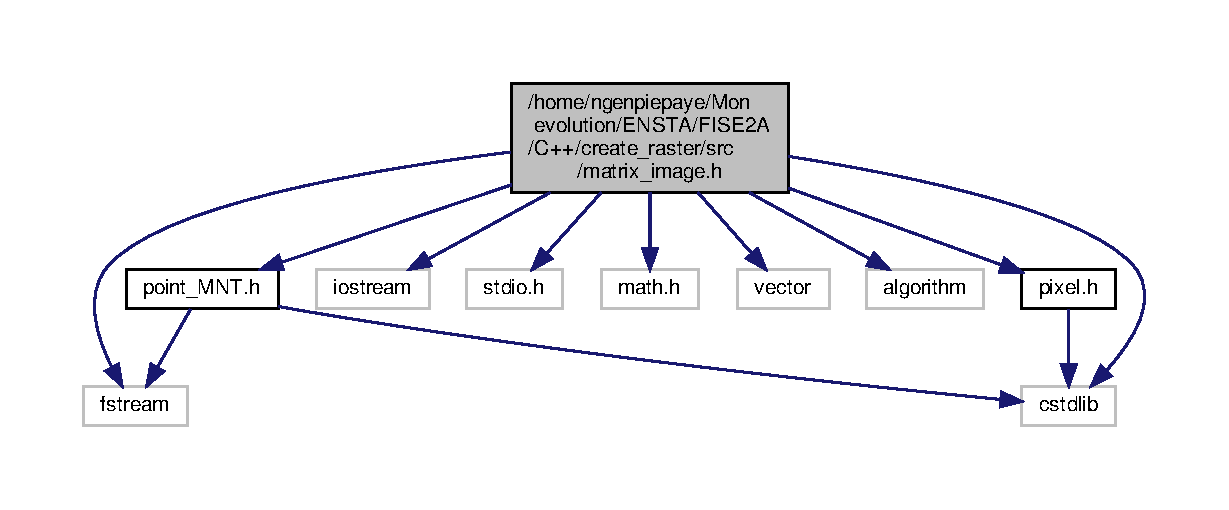
\includegraphics[width=350pt]{matrix__image_8h__incl}
\end{center}
\end{figure}
This graph shows which files directly or indirectly include this file\+:\nopagebreak
\begin{figure}[H]
\begin{center}
\leavevmode
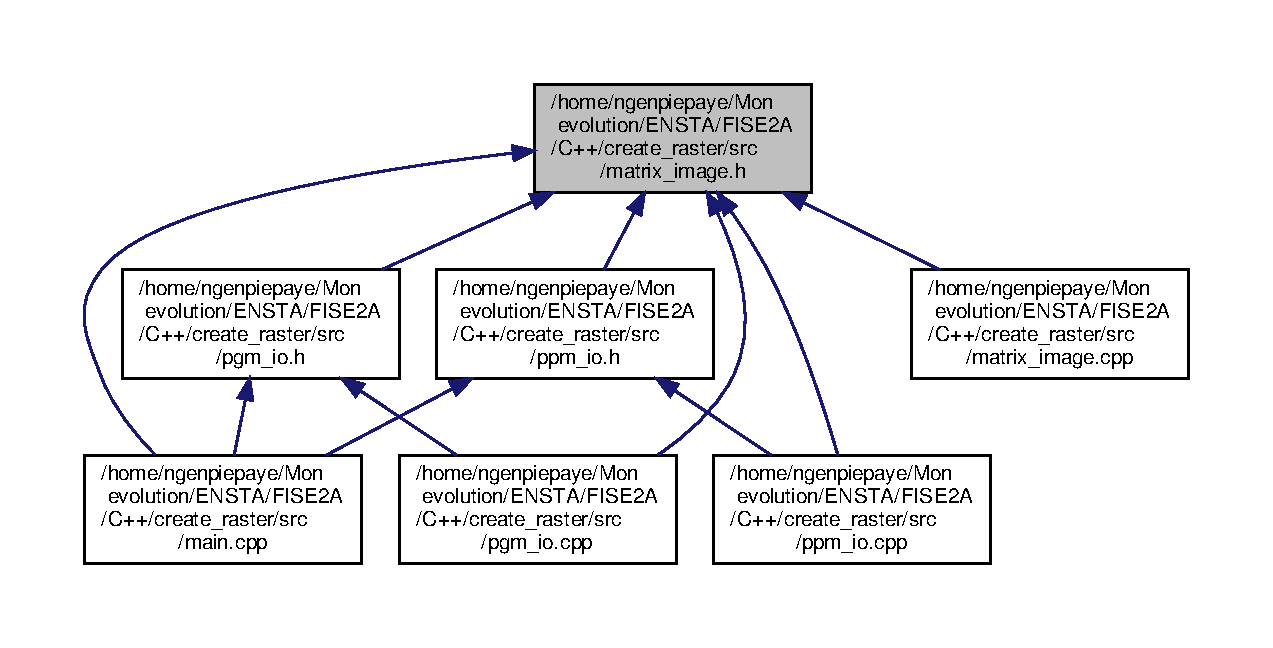
\includegraphics[width=350pt]{matrix__image_8h__dep__incl}
\end{center}
\end{figure}
\subsection*{Classes}
\begin{DoxyCompactItemize}
\item 
struct \hyperlink{struct_matrix__image}{Matrix\+\_\+image}
\end{DoxyCompactItemize}
\subsection*{Functions}
\begin{DoxyCompactItemize}
\item 
bool \hyperlink{matrix__image_8h_a621c37d96a7309382336d7efe143ff14}{compx} (const \hyperlink{class_point}{Point} \&p1, const \hyperlink{class_point}{Point} \&p2)
\item 
bool \hyperlink{matrix__image_8h_a10418f2e697e64aa06d030e2c6380464}{compy} (const \hyperlink{class_point}{Point} \&p1, const \hyperlink{class_point}{Point} \&p2)
\item 
bool \hyperlink{matrix__image_8h_a4de98c177b2c83ccf77dbb1cc2e266a7}{compz} (const \hyperlink{class_point}{Point} \&p1, const \hyperlink{class_point}{Point} \&p2)
\item 
void \hyperlink{matrix__image_8h_a1248e095df9c969f43fe954f9030236b}{readdata} (const string \&file\+\_\+name, vector$<$ \hyperlink{class_point}{Point} $>$ \&v\+\_\+\+Point)
\item 
void \hyperlink{matrix__image_8h_a25661ba2304c5f5ac7dd0faee662490a}{init\+\_\+\+Matrix\+\_\+image} (\hyperlink{struct_matrix__image}{Matrix\+\_\+image} \&matrix, int xsize, int ysize)
\item 
void \hyperlink{matrix__image_8h_a7ec590a2c385199d60e2e2f745b47193}{setup\+\_\+index\+\_\+pixel} (vector$<$ \hyperlink{class_point}{Point} $>$ \&v\+\_\+\+Point, \hyperlink{struct_matrix__image}{Matrix\+\_\+image} \&matrix)
\item 
void \hyperlink{matrix__image_8h_a6260293731b54842c441b7d643433469}{setup\+\_\+value\+\_\+pixel} (\hyperlink{struct_matrix__image}{Matrix\+\_\+image} \&matrix, vector$<$ \hyperlink{class_point}{Point} $>$ \&v\+\_\+\+Point)
\item 
void \hyperlink{matrix__image_8h_a8edbd41f8186f1314ce9b89466daa6a7}{set\+\_\+shadow} (\hyperlink{struct_matrix__image}{Matrix\+\_\+image} \&matrix, float Altitude, float Azimuth, float cellsize)
\end{DoxyCompactItemize}


\subsection{Function Documentation}
\mbox{\Hypertarget{matrix__image_8h_a621c37d96a7309382336d7efe143ff14}\label{matrix__image_8h_a621c37d96a7309382336d7efe143ff14}} 
\index{matrix\+\_\+image.\+h@{matrix\+\_\+image.\+h}!compx@{compx}}
\index{compx@{compx}!matrix\+\_\+image.\+h@{matrix\+\_\+image.\+h}}
\subsubsection{\texorpdfstring{compx()}{compx()}}
{\footnotesize\ttfamily bool compx (\begin{DoxyParamCaption}\item[{const \hyperlink{class_point}{Point} \&}]{p1,  }\item[{const \hyperlink{class_point}{Point} \&}]{p2 }\end{DoxyParamCaption})}

~\newline
$\ast$$\ast$$\ast$$\ast$$\ast$$\ast$$\ast$$\ast$$\ast$$\ast$$\ast$$\ast$$\ast$$\ast$$\ast$$\ast$$\ast$$\ast$$\ast$$\ast$$\ast$$\ast$$\ast$$\ast$$\ast$$\ast$$\ast$$\ast$$\ast$$\ast$$\ast$$\ast$$\ast$$\ast$$\ast$$\ast$$\ast$$\ast$$\ast$$\ast$$\ast$$\ast$$\ast$$\ast$$\ast$$\ast$$\ast$$\ast$$\ast$$\ast$$\ast$$\ast$$\ast$$\ast$$\ast$$\ast$$\ast$$\ast$$\ast$$\ast$$\ast$$\ast$$\ast$$\ast$$\ast$$\ast$$\ast$$\ast$$\ast$$\ast$$\ast$$\ast$$\ast$$\ast$$\ast$$\ast$ ~\newline
\textbackslash{} ~\newline
\textbackslash{} Purpose\+: ~\newline
\textbackslash{} ~\newline
\textbackslash{} Compare two points using the x coordinate of points ~\newline
\textbackslash{} ~\newline
\textbackslash{} example ~\newline
\textbackslash{} ~\newline
\textbackslash{} P1(5, 2, 8) , P2(3, 7, 4) ==$>$ P1 $>$ P2 ~\newline
\textbackslash{} ~\newline
\textbackslash{} Author\+: ~\newline
\textbackslash{} ~\newline
\textbackslash{} Stephane N\+G\+N\+E\+P\+I\+E\+P\+A\+YE W\+E\+M\+BE ~\newline
\textbackslash{} ~\newline
\textbackslash{} Parameters\+: ~\newline
\textbackslash{} ~\newline
\textbackslash{} Input, const \hyperlink{class_point}{Point}\& p1, the first point to compare. ~\newline
\textbackslash{} ~\newline
\textbackslash{} Input, const \hyperlink{class_point}{Point}\& p2, the second point to compare. ~\newline
\textbackslash{} ~\newline


Definition at line 15 of file matrix\+\_\+image.\+cpp.

\mbox{\Hypertarget{matrix__image_8h_a10418f2e697e64aa06d030e2c6380464}\label{matrix__image_8h_a10418f2e697e64aa06d030e2c6380464}} 
\index{matrix\+\_\+image.\+h@{matrix\+\_\+image.\+h}!compy@{compy}}
\index{compy@{compy}!matrix\+\_\+image.\+h@{matrix\+\_\+image.\+h}}
\subsubsection{\texorpdfstring{compy()}{compy()}}
{\footnotesize\ttfamily bool compy (\begin{DoxyParamCaption}\item[{const \hyperlink{class_point}{Point} \&}]{p1,  }\item[{const \hyperlink{class_point}{Point} \&}]{p2 }\end{DoxyParamCaption})}

~\newline
$\ast$$\ast$$\ast$$\ast$$\ast$$\ast$$\ast$$\ast$$\ast$$\ast$$\ast$$\ast$$\ast$$\ast$$\ast$$\ast$$\ast$$\ast$$\ast$$\ast$$\ast$$\ast$$\ast$$\ast$$\ast$$\ast$$\ast$$\ast$$\ast$$\ast$$\ast$$\ast$$\ast$$\ast$$\ast$$\ast$$\ast$$\ast$$\ast$$\ast$$\ast$$\ast$$\ast$$\ast$$\ast$$\ast$$\ast$$\ast$$\ast$$\ast$$\ast$$\ast$$\ast$$\ast$$\ast$$\ast$$\ast$$\ast$$\ast$$\ast$$\ast$$\ast$$\ast$$\ast$$\ast$$\ast$$\ast$$\ast$$\ast$$\ast$$\ast$$\ast$$\ast$$\ast$$\ast$$\ast$ ~\newline
\textbackslash{} ~\newline
\textbackslash{} Purpose\+: ~\newline
\textbackslash{} ~\newline
\textbackslash{} Compare two points using the y coordinate of points ~\newline
\textbackslash{} ~\newline
\textbackslash{} example ~\newline
\textbackslash{} ~\newline
\textbackslash{} P1(5, 2, 8) , P2(3, 7, 4) ==$>$ P2 $>$ P1 ~\newline
\textbackslash{} ~\newline
\textbackslash{} Author\+: ~\newline
\textbackslash{} ~\newline
\textbackslash{} Stephane N\+G\+N\+E\+P\+I\+E\+P\+A\+YE W\+E\+M\+BE ~\newline
\textbackslash{} ~\newline
\textbackslash{} Parameters\+: ~\newline
\textbackslash{} ~\newline
\textbackslash{} Input, const \hyperlink{class_point}{Point}\& p1, the first point to compare. ~\newline
\textbackslash{} ~\newline
\textbackslash{} Input, const \hyperlink{class_point}{Point}\& p2, the second point to compare. ~\newline
\textbackslash{} ~\newline


Definition at line 45 of file matrix\+\_\+image.\+cpp.

\mbox{\Hypertarget{matrix__image_8h_a4de98c177b2c83ccf77dbb1cc2e266a7}\label{matrix__image_8h_a4de98c177b2c83ccf77dbb1cc2e266a7}} 
\index{matrix\+\_\+image.\+h@{matrix\+\_\+image.\+h}!compz@{compz}}
\index{compz@{compz}!matrix\+\_\+image.\+h@{matrix\+\_\+image.\+h}}
\subsubsection{\texorpdfstring{compz()}{compz()}}
{\footnotesize\ttfamily bool compz (\begin{DoxyParamCaption}\item[{const \hyperlink{class_point}{Point} \&}]{p1,  }\item[{const \hyperlink{class_point}{Point} \&}]{p2 }\end{DoxyParamCaption})}

~\newline
$\ast$$\ast$$\ast$$\ast$$\ast$$\ast$$\ast$$\ast$$\ast$$\ast$$\ast$$\ast$$\ast$$\ast$$\ast$$\ast$$\ast$$\ast$$\ast$$\ast$$\ast$$\ast$$\ast$$\ast$$\ast$$\ast$$\ast$$\ast$$\ast$$\ast$$\ast$$\ast$$\ast$$\ast$$\ast$$\ast$$\ast$$\ast$$\ast$$\ast$$\ast$$\ast$$\ast$$\ast$$\ast$$\ast$$\ast$$\ast$$\ast$$\ast$$\ast$$\ast$$\ast$$\ast$$\ast$$\ast$$\ast$$\ast$$\ast$$\ast$$\ast$$\ast$$\ast$$\ast$$\ast$$\ast$$\ast$$\ast$$\ast$$\ast$$\ast$$\ast$$\ast$$\ast$$\ast$$\ast$ ~\newline
\textbackslash{} ~\newline
\textbackslash{} Purpose\+: ~\newline
\textbackslash{} ~\newline
\textbackslash{} Compare two points using the z coordinate of points ~\newline
\textbackslash{} ~\newline
\textbackslash{} example ~\newline
\textbackslash{} ~\newline
\textbackslash{} P1(5, 2, 8) , P2(3, 7, 4) ==$>$ P1 $>$ P2 ~\newline
\textbackslash{} ~\newline
\textbackslash{} Author\+: ~\newline
\textbackslash{} ~\newline
\textbackslash{} Stephane N\+G\+N\+E\+P\+I\+E\+P\+A\+YE W\+E\+M\+BE ~\newline
\textbackslash{} ~\newline
\textbackslash{} Parameters\+: ~\newline
\textbackslash{} ~\newline
\textbackslash{} Input, const \hyperlink{class_point}{Point}\& p1, the first point to compare. ~\newline
\textbackslash{} ~\newline
\textbackslash{} Input, const \hyperlink{class_point}{Point}\& p2, the second point to compare. ~\newline
\textbackslash{} ~\newline


Definition at line 75 of file matrix\+\_\+image.\+cpp.

\mbox{\Hypertarget{matrix__image_8h_a25661ba2304c5f5ac7dd0faee662490a}\label{matrix__image_8h_a25661ba2304c5f5ac7dd0faee662490a}} 
\index{matrix\+\_\+image.\+h@{matrix\+\_\+image.\+h}!init\+\_\+\+Matrix\+\_\+image@{init\+\_\+\+Matrix\+\_\+image}}
\index{init\+\_\+\+Matrix\+\_\+image@{init\+\_\+\+Matrix\+\_\+image}!matrix\+\_\+image.\+h@{matrix\+\_\+image.\+h}}
\subsubsection{\texorpdfstring{init\+\_\+\+Matrix\+\_\+image()}{init\_Matrix\_image()}}
{\footnotesize\ttfamily void init\+\_\+\+Matrix\+\_\+image (\begin{DoxyParamCaption}\item[{\hyperlink{struct_matrix__image}{Matrix\+\_\+image} \&}]{matrix,  }\item[{int}]{xsize,  }\item[{int}]{ysize }\end{DoxyParamCaption})}

~\newline
$\ast$$\ast$$\ast$$\ast$$\ast$$\ast$$\ast$$\ast$$\ast$$\ast$$\ast$$\ast$$\ast$$\ast$$\ast$$\ast$$\ast$$\ast$$\ast$$\ast$$\ast$$\ast$$\ast$$\ast$$\ast$$\ast$$\ast$$\ast$$\ast$$\ast$$\ast$$\ast$$\ast$$\ast$$\ast$$\ast$$\ast$$\ast$$\ast$$\ast$$\ast$$\ast$$\ast$$\ast$$\ast$$\ast$$\ast$$\ast$$\ast$$\ast$$\ast$$\ast$$\ast$$\ast$$\ast$$\ast$$\ast$$\ast$$\ast$$\ast$$\ast$$\ast$$\ast$$\ast$$\ast$$\ast$$\ast$$\ast$$\ast$$\ast$$\ast$$\ast$$\ast$$\ast$$\ast$$\ast$ ~\newline
\textbackslash{} ~\newline
\textbackslash{} Purpose\+:~\newline
\textbackslash{} ~\newline
\textbackslash{} Create a matrix of pixel and initialize these pixels ~\newline
\textbackslash{} ~\newline
\textbackslash{} Author\+: ~\newline
\textbackslash{} ~\newline
\textbackslash{} Stephane N\+G\+N\+E\+P\+I\+E\+P\+A\+YE W\+E\+M\+BE ~\newline
\textbackslash{} ~\newline
\textbackslash{} Parameters\+: ~\newline
\textbackslash{} ~\newline
\textbackslash{} Input, \hyperlink{struct_matrix__image}{Matrix\+\_\+image}\& matrix, matrix of pixels of the image ~\newline
\textbackslash{} Input, const int\& xsize, the whith of the image (number of pixels on the whidth) ~\newline
\textbackslash{} Input, int\& ysize, the height of the image (number of pixels on the heigth) ~\newline
\textbackslash{} ~\newline


Definition at line 160 of file matrix\+\_\+image.\+cpp.

\mbox{\Hypertarget{matrix__image_8h_a1248e095df9c969f43fe954f9030236b}\label{matrix__image_8h_a1248e095df9c969f43fe954f9030236b}} 
\index{matrix\+\_\+image.\+h@{matrix\+\_\+image.\+h}!readdata@{readdata}}
\index{readdata@{readdata}!matrix\+\_\+image.\+h@{matrix\+\_\+image.\+h}}
\subsubsection{\texorpdfstring{readdata()}{readdata()}}
{\footnotesize\ttfamily void readdata (\begin{DoxyParamCaption}\item[{const string \&}]{file\+\_\+name,  }\item[{vector$<$ \hyperlink{class_point}{Point} $>$ \&}]{v\+\_\+\+Point }\end{DoxyParamCaption})}

~\newline
$\ast$$\ast$$\ast$$\ast$$\ast$$\ast$$\ast$$\ast$$\ast$$\ast$$\ast$$\ast$$\ast$$\ast$$\ast$$\ast$$\ast$$\ast$$\ast$$\ast$$\ast$$\ast$$\ast$$\ast$$\ast$$\ast$$\ast$$\ast$$\ast$$\ast$$\ast$$\ast$$\ast$$\ast$$\ast$$\ast$$\ast$$\ast$$\ast$$\ast$$\ast$$\ast$$\ast$$\ast$$\ast$$\ast$$\ast$$\ast$$\ast$$\ast$$\ast$$\ast$$\ast$$\ast$$\ast$$\ast$$\ast$$\ast$$\ast$$\ast$$\ast$$\ast$$\ast$$\ast$$\ast$$\ast$$\ast$$\ast$$\ast$$\ast$$\ast$$\ast$$\ast$$\ast$$\ast$$\ast$$\ast$ ~\newline
\textbackslash{} ~\newline
\textbackslash{} Purpose\+: ~\newline
\textbackslash{} ~\newline
\textbackslash{} Extract data of the M\+NT and put them inside a vector ~\newline
\textbackslash{} ~\newline
\textbackslash{} example ~\newline
\textbackslash{} ~\newline
\textbackslash{} 48.\+19517461 -\/3.\+028930672 -\/117.\+281 ~\newline
\textbackslash{} 48.\+19517496 -\/3.\+028923963 -\/117.\+469 ~\newline
\textbackslash{} 48.\+1951753 -\/3.\+028917253 -\/117.\+527 ~\newline
\textbackslash{} 48.\+19517564 -\/3.\+028910544 -\/117.\+506 ~\newline
\textbackslash{} 48.\+19517738 -\/3.\+028964733 -\/116.\+976 ~\newline
\textbackslash{} ..... ~\newline
\textbackslash{} ~\newline
\textbackslash{} Author\+: ~\newline
\textbackslash{} ~\newline
\textbackslash{} Stephane N\+G\+N\+E\+P\+I\+E\+P\+A\+YE W\+E\+M\+BE ~\newline
\textbackslash{} ~\newline
\textbackslash{} Parameters\+: ~\newline
\textbackslash{} ~\newline
\textbackslash{} Input, const string\& file\+\_\+name, the name of the file containing data to extract. ~\newline
\textbackslash{} ~\newline
\textbackslash{} Input, vector$<$\+Point$>$\& v\+\_\+\+Point, the vector to fill. ~\newline
\textbackslash{} ~\newline


Definition at line 105 of file matrix\+\_\+image.\+cpp.

\mbox{\Hypertarget{matrix__image_8h_a8edbd41f8186f1314ce9b89466daa6a7}\label{matrix__image_8h_a8edbd41f8186f1314ce9b89466daa6a7}} 
\index{matrix\+\_\+image.\+h@{matrix\+\_\+image.\+h}!set\+\_\+shadow@{set\+\_\+shadow}}
\index{set\+\_\+shadow@{set\+\_\+shadow}!matrix\+\_\+image.\+h@{matrix\+\_\+image.\+h}}
\subsubsection{\texorpdfstring{set\+\_\+shadow()}{set\_shadow()}}
{\footnotesize\ttfamily void set\+\_\+shadow (\begin{DoxyParamCaption}\item[{\hyperlink{struct_matrix__image}{Matrix\+\_\+image} \&}]{matrix,  }\item[{float}]{Altitude,  }\item[{float}]{Azimuth,  }\item[{float}]{cellsize }\end{DoxyParamCaption})}

~\newline
$\ast$$\ast$$\ast$$\ast$$\ast$$\ast$$\ast$$\ast$$\ast$$\ast$$\ast$$\ast$$\ast$$\ast$$\ast$$\ast$$\ast$$\ast$$\ast$$\ast$$\ast$$\ast$$\ast$$\ast$$\ast$$\ast$$\ast$$\ast$$\ast$$\ast$$\ast$$\ast$$\ast$$\ast$$\ast$$\ast$$\ast$$\ast$$\ast$$\ast$$\ast$$\ast$$\ast$$\ast$$\ast$$\ast$$\ast$$\ast$$\ast$$\ast$$\ast$$\ast$$\ast$$\ast$$\ast$$\ast$$\ast$$\ast$$\ast$$\ast$$\ast$$\ast$$\ast$$\ast$$\ast$$\ast$$\ast$$\ast$$\ast$$\ast$$\ast$$\ast$$\ast$$\ast$$\ast$$\ast$ ~\newline
\textbackslash{} ~\newline
\textbackslash{} Purpose\+:~\newline
\textbackslash{} ~\newline
\textbackslash{} mise de l\textquotesingle{}ombrage mais ne fonctionne pas encore ~\newline
\textbackslash{} ~\newline
\textbackslash{} Author\+:~\newline
\textbackslash{} ~\newline
\textbackslash{} Stephane N\+G\+N\+E\+P\+I\+E\+P\+A\+YE W\+E\+M\+BE ~\newline
\textbackslash{} ~\newline
\textbackslash{} Parameters\+: ~\newline
\textbackslash{} ~\newline
\textbackslash{} Input, \hyperlink{struct_matrix__image}{Matrix\+\_\+image}\& matrix, matrix of pixels of the image ~\newline
\textbackslash{} ~\newline


Definition at line 309 of file matrix\+\_\+image.\+cpp.

\mbox{\Hypertarget{matrix__image_8h_a7ec590a2c385199d60e2e2f745b47193}\label{matrix__image_8h_a7ec590a2c385199d60e2e2f745b47193}} 
\index{matrix\+\_\+image.\+h@{matrix\+\_\+image.\+h}!setup\+\_\+index\+\_\+pixel@{setup\+\_\+index\+\_\+pixel}}
\index{setup\+\_\+index\+\_\+pixel@{setup\+\_\+index\+\_\+pixel}!matrix\+\_\+image.\+h@{matrix\+\_\+image.\+h}}
\subsubsection{\texorpdfstring{setup\+\_\+index\+\_\+pixel()}{setup\_index\_pixel()}}
{\footnotesize\ttfamily void setup\+\_\+index\+\_\+pixel (\begin{DoxyParamCaption}\item[{vector$<$ \hyperlink{class_point}{Point} $>$ \&}]{v\+\_\+\+Point,  }\item[{\hyperlink{struct_matrix__image}{Matrix\+\_\+image} \&}]{matrix }\end{DoxyParamCaption})}

~\newline
$\ast$$\ast$$\ast$$\ast$$\ast$$\ast$$\ast$$\ast$$\ast$$\ast$$\ast$$\ast$$\ast$$\ast$$\ast$$\ast$$\ast$$\ast$$\ast$$\ast$$\ast$$\ast$$\ast$$\ast$$\ast$$\ast$$\ast$$\ast$$\ast$$\ast$$\ast$$\ast$$\ast$$\ast$$\ast$$\ast$$\ast$$\ast$$\ast$$\ast$$\ast$$\ast$$\ast$$\ast$$\ast$$\ast$$\ast$$\ast$$\ast$$\ast$$\ast$$\ast$$\ast$$\ast$$\ast$$\ast$$\ast$$\ast$$\ast$$\ast$$\ast$$\ast$$\ast$$\ast$$\ast$$\ast$$\ast$$\ast$$\ast$$\ast$$\ast$$\ast$$\ast$$\ast$$\ast$$\ast$ ~\newline
\textbackslash{} ~\newline
\textbackslash{} Purpose\+: ~\newline
\textbackslash{} ~\newline
\textbackslash{} Set up of index of pixel inside the pixel matrix of the image ~\newline
\textbackslash{} for each element of list of point of the M\+NT we find which pixel corresponding to that point ~\newline
\textbackslash{} ~\newline
\textbackslash{} Author\+:~\newline
\textbackslash{} ~\newline
\textbackslash{} Stephane N\+G\+N\+E\+P\+I\+E\+P\+A\+YE W\+E\+M\+BE ~\newline
\textbackslash{} ~\newline
\textbackslash{} Parameters\+: ~\newline
\textbackslash{} ~\newline
\textbackslash{} Input, vector$<$\+Point$>$\& v\+\_\+\+Point, the vector of all points of the M\+NT. ~\newline
\textbackslash{} Input, \hyperlink{struct_matrix__image}{Matrix\+\_\+image}\& matrix, the matrix which containt all pixel of the image to set up ~\newline
\textbackslash{} ~\newline


Definition at line 202 of file matrix\+\_\+image.\+cpp.

\mbox{\Hypertarget{matrix__image_8h_a6260293731b54842c441b7d643433469}\label{matrix__image_8h_a6260293731b54842c441b7d643433469}} 
\index{matrix\+\_\+image.\+h@{matrix\+\_\+image.\+h}!setup\+\_\+value\+\_\+pixel@{setup\+\_\+value\+\_\+pixel}}
\index{setup\+\_\+value\+\_\+pixel@{setup\+\_\+value\+\_\+pixel}!matrix\+\_\+image.\+h@{matrix\+\_\+image.\+h}}
\subsubsection{\texorpdfstring{setup\+\_\+value\+\_\+pixel()}{setup\_value\_pixel()}}
{\footnotesize\ttfamily void setup\+\_\+value\+\_\+pixel (\begin{DoxyParamCaption}\item[{\hyperlink{struct_matrix__image}{Matrix\+\_\+image} \&}]{matrix,  }\item[{vector$<$ \hyperlink{class_point}{Point} $>$ \&}]{v\+\_\+\+Point }\end{DoxyParamCaption})}

~\newline
$\ast$$\ast$$\ast$$\ast$$\ast$$\ast$$\ast$$\ast$$\ast$$\ast$$\ast$$\ast$$\ast$$\ast$$\ast$$\ast$$\ast$$\ast$$\ast$$\ast$$\ast$$\ast$$\ast$$\ast$$\ast$$\ast$$\ast$$\ast$$\ast$$\ast$$\ast$$\ast$$\ast$$\ast$$\ast$$\ast$$\ast$$\ast$$\ast$$\ast$$\ast$$\ast$$\ast$$\ast$$\ast$$\ast$$\ast$$\ast$$\ast$$\ast$$\ast$$\ast$$\ast$$\ast$$\ast$$\ast$$\ast$$\ast$$\ast$$\ast$$\ast$$\ast$$\ast$$\ast$$\ast$$\ast$$\ast$$\ast$$\ast$$\ast$$\ast$$\ast$$\ast$$\ast$$\ast$$\ast$ ~\newline
\textbackslash{} ~\newline
\textbackslash{} Purpose\+: ~\newline
\textbackslash{} ~\newline
\textbackslash{} Set up of the value of pixel inside the pixel matrix of the image ~\newline
\textbackslash{} ~\newline
\textbackslash{} Author\+:~\newline
\textbackslash{} ~\newline
\textbackslash{} Stephane N\+G\+N\+E\+P\+I\+E\+P\+A\+YE W\+E\+M\+BE ~\newline
\textbackslash{} ~\newline
\textbackslash{} Parameters\+:~\newline
\textbackslash{} ~\newline
\textbackslash{} Input, vector$<$\+Point$>$\& v\+\_\+\+Point, the vector of all points of the M\+NT.~\newline
\textbackslash{} Input, \hyperlink{struct_matrix__image}{Matrix\+\_\+image}\& matrix, the matrix which containt all pixel of the image to set up~\newline
\textbackslash{} ~\newline


Definition at line 252 of file matrix\+\_\+image.\+cpp.


\hypertarget{pgm__io_8cpp}{}\section{/home/ngenpiepaye/\+Mon evolution/\+E\+N\+S\+T\+A/\+F\+I\+S\+E2\+A/\+C++/create\+\_\+raster/src/pgm\+\_\+io.cpp File Reference}
\label{pgm__io_8cpp}\index{/home/ngenpiepaye/\+Mon evolution/\+E\+N\+S\+T\+A/\+F\+I\+S\+E2\+A/\+C++/create\+\_\+raster/src/pgm\+\_\+io.\+cpp@{/home/ngenpiepaye/\+Mon evolution/\+E\+N\+S\+T\+A/\+F\+I\+S\+E2\+A/\+C++/create\+\_\+raster/src/pgm\+\_\+io.\+cpp}}
{\ttfamily \#include $<$cstdlib$>$}\newline
{\ttfamily \#include $<$iostream$>$}\newline
{\ttfamily \#include \char`\"{}matrix\+\_\+image.\+h\char`\"{}}\newline
{\ttfamily \#include \char`\"{}pixel.\+h\char`\"{}}\newline
{\ttfamily \#include \char`\"{}pgm\+\_\+io.\+h\char`\"{}}\newline
Include dependency graph for pgm\+\_\+io.\+cpp\+:\nopagebreak
\begin{figure}[H]
\begin{center}
\leavevmode
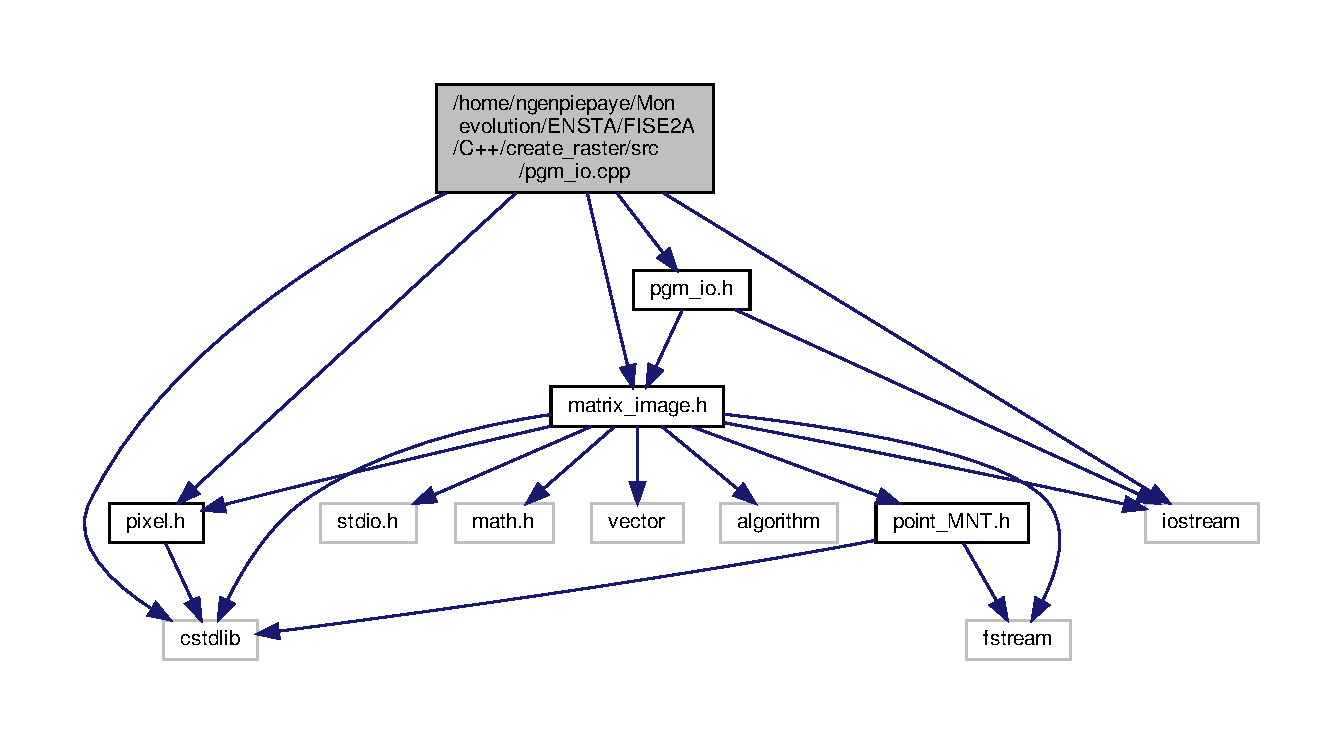
\includegraphics[width=350pt]{pgm__io_8cpp__incl}
\end{center}
\end{figure}
\subsection*{Functions}
\begin{DoxyCompactItemize}
\item 
void \hyperlink{pgm__io_8cpp_a31647643638446f50a111b320359fc71}{pgma\+\_\+write} (const string output\+\_\+name, const \hyperlink{struct_matrix__image}{Matrix\+\_\+image} \&matrix)
\item 
void \hyperlink{pgm__io_8cpp_acd3149f088e0122c2b30e1b40a7750a2}{pgma\+\_\+write\+\_\+data} (ofstream \&output, const \hyperlink{struct_matrix__image}{Matrix\+\_\+image} \&matrix)
\item 
void \hyperlink{pgm__io_8cpp_a10fec918da7d3c0767f34c55f4fc16a9}{pgma\+\_\+write\+\_\+header} (ofstream \&output, const string output\+\_\+name, const \hyperlink{struct_matrix__image}{Matrix\+\_\+image} \&matrix, const unsigned int maxg)
\item 
void \hyperlink{pgm__io_8cpp_a7b2bdbbc65ad268b966ccc7e36c86bb6}{pgmb\+\_\+write} (const string output\+\_\+name, const \hyperlink{struct_matrix__image}{Matrix\+\_\+image} \&matrix)
\item 
void \hyperlink{pgm__io_8cpp_a4c2952163ded78067fb83bd465034f85}{pgmb\+\_\+write\+\_\+data} (ofstream \&output, const \hyperlink{struct_matrix__image}{Matrix\+\_\+image} \&matrix)
\item 
void \hyperlink{pgm__io_8cpp_a77d494aebd0a550099d634f486ef8a39}{pgmb\+\_\+write\+\_\+header} (ofstream \&output, const string output\+\_\+name, const \hyperlink{struct_matrix__image}{Matrix\+\_\+image} \&matrix, const unsigned int maxg)
\end{DoxyCompactItemize}


\subsection{Function Documentation}
\mbox{\Hypertarget{pgm__io_8cpp_a31647643638446f50a111b320359fc71}\label{pgm__io_8cpp_a31647643638446f50a111b320359fc71}} 
\index{pgm\+\_\+io.\+cpp@{pgm\+\_\+io.\+cpp}!pgma\+\_\+write@{pgma\+\_\+write}}
\index{pgma\+\_\+write@{pgma\+\_\+write}!pgm\+\_\+io.\+cpp@{pgm\+\_\+io.\+cpp}}
\subsubsection{\texorpdfstring{pgma\+\_\+write()}{pgma\_write()}}
{\footnotesize\ttfamily void pgma\+\_\+write (\begin{DoxyParamCaption}\item[{const string}]{output\+\_\+name,  }\item[{const \hyperlink{struct_matrix__image}{Matrix\+\_\+image} \&}]{matrix }\end{DoxyParamCaption})}

~\newline
$\ast$$\ast$$\ast$$\ast$$\ast$$\ast$$\ast$$\ast$$\ast$$\ast$$\ast$$\ast$$\ast$$\ast$$\ast$$\ast$$\ast$$\ast$$\ast$$\ast$$\ast$$\ast$$\ast$$\ast$$\ast$$\ast$$\ast$$\ast$$\ast$$\ast$$\ast$$\ast$$\ast$$\ast$$\ast$$\ast$$\ast$$\ast$$\ast$$\ast$$\ast$$\ast$$\ast$$\ast$$\ast$$\ast$$\ast$$\ast$$\ast$$\ast$$\ast$$\ast$$\ast$$\ast$$\ast$$\ast$$\ast$$\ast$$\ast$$\ast$$\ast$$\ast$$\ast$$\ast$$\ast$$\ast$$\ast$$\ast$$\ast$$\ast$$\ast$$\ast$$\ast$$\ast$$\ast$$\ast$~\newline
\textbackslash{} ~\newline
\textbackslash{} Purpose\+:~\newline
\textbackslash{} ~\newline
\textbackslash{} P\+G\+M\+A\+\_\+\+W\+R\+I\+TE writes the header and data for an A\+S\+C\+II P\+GM file.~\newline
\textbackslash{} ~\newline
\textbackslash{} Example\+:~\newline
\textbackslash{} ~\newline
\textbackslash{} P2~\newline
\textbackslash{} \# feep.\+pgm~\newline
\textbackslash{} 24 7~\newline
\textbackslash{} 15~\newline
\textbackslash{} 0 0 0 0 0 0 0 0 0 0 0 0 0 0 0 0 0 0 0 0 0 0 0 0~\newline
\textbackslash{} 0 3 3 3 3 0 0 7 7 7 7 0 0 11 11 11 11 0 0 15 15 15 15 0~\newline
\textbackslash{} 0 3 0 0 0 0 0 7 0 0 0 0 0 11 0 0 0 0 0 15 0 0 15 0~\newline
\textbackslash{} 0 3 3 3 0 0 0 7 7 7 0 0 0 11 11 11 0 0 0 15 15 15 15 0~\newline
\textbackslash{} 0 3 0 0 0 0 0 7 0 0 0 0 0 11 0 0 0 0 0 15 0 0 0 0~\newline
\textbackslash{} 0 3 0 0 0 0 0 7 7 7 7 0 0 11 11 11 11 0 0 15 0 0 0 0~\newline
\textbackslash{} 0 0 0 0 0 0 0 0 0 0 0 0 0 0 0 0 0 0 0 0 0 0 0 0~\newline
\textbackslash{} ~\newline
\textbackslash{} Author\+:~\newline
\textbackslash{} ~\newline
\textbackslash{} stephane N\+G\+N\+E\+P\+I\+E\+P\+A\+YE W\+E\+M\+BE~\newline
\textbackslash{} ~\newline
\textbackslash{} Parameters\+:~\newline
\textbackslash{} ~\newline
\textbackslash{} Input, string O\+U\+T\+P\+U\+T\+\_\+\+N\+A\+ME, the name of the file.~\newline
\textbackslash{} ~\newline
\textbackslash{} Input, \hyperlink{struct_matrix__image}{Matrix\+\_\+image}\& matrix matrix of pixel.~\newline
\textbackslash{} ~\newline


Definition at line 12 of file pgm\+\_\+io.\+cpp.

\mbox{\Hypertarget{pgm__io_8cpp_acd3149f088e0122c2b30e1b40a7750a2}\label{pgm__io_8cpp_acd3149f088e0122c2b30e1b40a7750a2}} 
\index{pgm\+\_\+io.\+cpp@{pgm\+\_\+io.\+cpp}!pgma\+\_\+write\+\_\+data@{pgma\+\_\+write\+\_\+data}}
\index{pgma\+\_\+write\+\_\+data@{pgma\+\_\+write\+\_\+data}!pgm\+\_\+io.\+cpp@{pgm\+\_\+io.\+cpp}}
\subsubsection{\texorpdfstring{pgma\+\_\+write\+\_\+data()}{pgma\_write\_data()}}
{\footnotesize\ttfamily void pgma\+\_\+write\+\_\+data (\begin{DoxyParamCaption}\item[{ofstream \&}]{output,  }\item[{const \hyperlink{struct_matrix__image}{Matrix\+\_\+image} \&}]{matrix }\end{DoxyParamCaption})}

~\newline
$\ast$$\ast$$\ast$$\ast$$\ast$$\ast$$\ast$$\ast$$\ast$$\ast$$\ast$$\ast$$\ast$$\ast$$\ast$$\ast$$\ast$$\ast$$\ast$$\ast$$\ast$$\ast$$\ast$$\ast$$\ast$$\ast$$\ast$$\ast$$\ast$$\ast$$\ast$$\ast$$\ast$$\ast$$\ast$$\ast$$\ast$$\ast$$\ast$$\ast$$\ast$$\ast$$\ast$$\ast$$\ast$$\ast$$\ast$$\ast$$\ast$$\ast$$\ast$$\ast$$\ast$$\ast$$\ast$$\ast$$\ast$$\ast$$\ast$$\ast$$\ast$$\ast$$\ast$$\ast$$\ast$$\ast$$\ast$$\ast$$\ast$$\ast$$\ast$$\ast$$\ast$$\ast$$\ast$$\ast$~\newline
\textbackslash{} ~\newline
\textbackslash{} Purpose\+:~\newline
\textbackslash{} ~\newline
\textbackslash{} P\+G\+M\+A\+\_\+\+W\+R\+I\+T\+E\+\_\+\+D\+A\+TA writes the data for an A\+S\+C\+II P\+GM file.~\newline
\textbackslash{} ~\newline
\textbackslash{} Author\+:~\newline
\textbackslash{} ~\newline
\textbackslash{} Stephane N\+G\+N\+E\+P\+I\+E\+P\+A\+YE W\+E\+M\+BE~\newline
\textbackslash{} ~\newline
\textbackslash{} Parameters\+:~\newline
\textbackslash{} ~\newline
\textbackslash{} Input, ofstream \&O\+U\+T\+P\+UT, a pointer to the file.~\newline
\textbackslash{} ~\newline
\textbackslash{} Input, \hyperlink{struct_matrix__image}{Matrix\+\_\+image}\& matrix matrix of pixel.~\newline
\textbackslash{} ~\newline


Definition at line 97 of file pgm\+\_\+io.\+cpp.

\mbox{\Hypertarget{pgm__io_8cpp_a10fec918da7d3c0767f34c55f4fc16a9}\label{pgm__io_8cpp_a10fec918da7d3c0767f34c55f4fc16a9}} 
\index{pgm\+\_\+io.\+cpp@{pgm\+\_\+io.\+cpp}!pgma\+\_\+write\+\_\+header@{pgma\+\_\+write\+\_\+header}}
\index{pgma\+\_\+write\+\_\+header@{pgma\+\_\+write\+\_\+header}!pgm\+\_\+io.\+cpp@{pgm\+\_\+io.\+cpp}}
\subsubsection{\texorpdfstring{pgma\+\_\+write\+\_\+header()}{pgma\_write\_header()}}
{\footnotesize\ttfamily void pgma\+\_\+write\+\_\+header (\begin{DoxyParamCaption}\item[{ofstream \&}]{output,  }\item[{const string}]{output\+\_\+name,  }\item[{const \hyperlink{struct_matrix__image}{Matrix\+\_\+image} \&}]{matrix,  }\item[{const unsigned int}]{maxg }\end{DoxyParamCaption})}

~\newline
$\ast$$\ast$$\ast$$\ast$$\ast$$\ast$$\ast$$\ast$$\ast$$\ast$$\ast$$\ast$$\ast$$\ast$$\ast$$\ast$$\ast$$\ast$$\ast$$\ast$$\ast$$\ast$$\ast$$\ast$$\ast$$\ast$$\ast$$\ast$$\ast$$\ast$$\ast$$\ast$$\ast$$\ast$$\ast$$\ast$$\ast$$\ast$$\ast$$\ast$$\ast$$\ast$$\ast$$\ast$$\ast$$\ast$$\ast$$\ast$$\ast$$\ast$$\ast$$\ast$$\ast$$\ast$$\ast$$\ast$$\ast$$\ast$$\ast$$\ast$$\ast$$\ast$$\ast$$\ast$$\ast$$\ast$$\ast$$\ast$$\ast$$\ast$$\ast$$\ast$$\ast$$\ast$$\ast$$\ast$~\newline
\textbackslash{} ~\newline
\textbackslash{} Purpose\+:~\newline
\textbackslash{} ~\newline
\textbackslash{} P\+G\+M\+A\+\_\+\+W\+R\+I\+T\+E\+\_\+\+H\+E\+A\+D\+ER writes the header of an A\+S\+C\+II P\+GM file.~\newline
\textbackslash{} ~\newline
\textbackslash{} Author\+:~\newline
\textbackslash{} ~\newline
\textbackslash{} Steĥane N\+G\+N\+E\+P\+I\+E\+P\+A\+YE W\+E\+M\+BE~\newline
\textbackslash{} ~\newline
\textbackslash{} Parameters\+:~\newline
\textbackslash{} ~\newline
\textbackslash{} Input, ofstream \&O\+U\+T\+P\+UT, a pointer to the file.~\newline
\textbackslash{} ~\newline
\textbackslash{} Input, string O\+U\+T\+P\+U\+T\+\_\+\+N\+A\+ME, the name of the file.~\newline
\textbackslash{} ~\newline
\textbackslash{} Input, \hyperlink{struct_matrix__image}{Matrix\+\_\+image}\& matrix matrix of pixel.~\newline
\textbackslash{} ~\newline
\textbackslash{} Input, unsigned int M\+A\+XG, the maximum gray value.~\newline
\textbackslash{} ~\newline


Definition at line 147 of file pgm\+\_\+io.\+cpp.

\mbox{\Hypertarget{pgm__io_8cpp_a7b2bdbbc65ad268b966ccc7e36c86bb6}\label{pgm__io_8cpp_a7b2bdbbc65ad268b966ccc7e36c86bb6}} 
\index{pgm\+\_\+io.\+cpp@{pgm\+\_\+io.\+cpp}!pgmb\+\_\+write@{pgmb\+\_\+write}}
\index{pgmb\+\_\+write@{pgmb\+\_\+write}!pgm\+\_\+io.\+cpp@{pgm\+\_\+io.\+cpp}}
\subsubsection{\texorpdfstring{pgmb\+\_\+write()}{pgmb\_write()}}
{\footnotesize\ttfamily void pgmb\+\_\+write (\begin{DoxyParamCaption}\item[{const string}]{output\+\_\+name,  }\item[{const \hyperlink{struct_matrix__image}{Matrix\+\_\+image} \&}]{matrix }\end{DoxyParamCaption})}

~\newline
$\ast$$\ast$$\ast$$\ast$$\ast$$\ast$$\ast$$\ast$$\ast$$\ast$$\ast$$\ast$$\ast$$\ast$$\ast$$\ast$$\ast$$\ast$$\ast$$\ast$$\ast$$\ast$$\ast$$\ast$$\ast$$\ast$$\ast$$\ast$$\ast$$\ast$$\ast$$\ast$$\ast$$\ast$$\ast$$\ast$$\ast$$\ast$$\ast$$\ast$$\ast$$\ast$$\ast$$\ast$$\ast$$\ast$$\ast$$\ast$$\ast$$\ast$$\ast$$\ast$$\ast$$\ast$$\ast$$\ast$$\ast$$\ast$$\ast$$\ast$$\ast$$\ast$$\ast$$\ast$$\ast$$\ast$$\ast$$\ast$$\ast$$\ast$$\ast$$\ast$$\ast$$\ast$$\ast$$\ast$~\newline
\textbackslash{} ~\newline
\textbackslash{} Purpose\+:~\newline
\textbackslash{} ~\newline
\textbackslash{} P\+G\+M\+B\+\_\+\+W\+R\+I\+TE writes the header and data for a binary P\+GM file.~\newline
\textbackslash{} ~\newline
\textbackslash{} example~\newline
\textbackslash{} ~\newline
\textbackslash{} P3~\newline
\textbackslash{} \# Le P3 signifie que les couleurs sont en A\+S\+C\+II, et qu\textquotesingle{}elles sont en R\+GB.~\newline
\textbackslash{} \# Par 3 colonnes et 2 lignes \+:~\newline
\textbackslash{} 3 2~\newline
\textbackslash{} \# Ayant 255 pour valeur maximum \+:~\newline
\textbackslash{} data ...~\newline
\textbackslash{} ~\newline
\textbackslash{} Author\+:~\newline
\textbackslash{} ~\newline
\textbackslash{} Stephane N\+G\+N\+E\+P\+I\+E\+P\+A\+YE W\+E\+M\+BE~\newline
\textbackslash{} ~\newline
\textbackslash{} Parameters\+:~\newline
\textbackslash{} ~\newline
\textbackslash{} Input, string O\+U\+T\+P\+U\+T\+\_\+\+N\+A\+ME, the name of the file.~\newline
\textbackslash{} ~\newline
\textbackslash{} Input, \hyperlink{struct_matrix__image}{Matrix\+\_\+image}\& matrix matrix of pixel.~\newline
\textbackslash{} ~\newline


Definition at line 182 of file pgm\+\_\+io.\+cpp.

\mbox{\Hypertarget{pgm__io_8cpp_a4c2952163ded78067fb83bd465034f85}\label{pgm__io_8cpp_a4c2952163ded78067fb83bd465034f85}} 
\index{pgm\+\_\+io.\+cpp@{pgm\+\_\+io.\+cpp}!pgmb\+\_\+write\+\_\+data@{pgmb\+\_\+write\+\_\+data}}
\index{pgmb\+\_\+write\+\_\+data@{pgmb\+\_\+write\+\_\+data}!pgm\+\_\+io.\+cpp@{pgm\+\_\+io.\+cpp}}
\subsubsection{\texorpdfstring{pgmb\+\_\+write\+\_\+data()}{pgmb\_write\_data()}}
{\footnotesize\ttfamily void pgmb\+\_\+write\+\_\+data (\begin{DoxyParamCaption}\item[{ofstream \&}]{output,  }\item[{const \hyperlink{struct_matrix__image}{Matrix\+\_\+image} \&}]{matrix }\end{DoxyParamCaption})}

~\newline
$\ast$$\ast$$\ast$$\ast$$\ast$$\ast$$\ast$$\ast$$\ast$$\ast$$\ast$$\ast$$\ast$$\ast$$\ast$$\ast$$\ast$$\ast$$\ast$$\ast$$\ast$$\ast$$\ast$$\ast$$\ast$$\ast$$\ast$$\ast$$\ast$$\ast$$\ast$$\ast$$\ast$$\ast$$\ast$$\ast$$\ast$$\ast$$\ast$$\ast$$\ast$$\ast$$\ast$$\ast$$\ast$$\ast$$\ast$$\ast$$\ast$$\ast$$\ast$$\ast$$\ast$$\ast$$\ast$$\ast$$\ast$$\ast$$\ast$$\ast$$\ast$$\ast$$\ast$$\ast$$\ast$$\ast$$\ast$$\ast$$\ast$$\ast$$\ast$$\ast$$\ast$$\ast$$\ast$$\ast$~\newline
\textbackslash{} ~\newline
\textbackslash{} Purpose\+:~\newline
\textbackslash{} ~\newline
\textbackslash{} P\+G\+M\+B\+\_\+\+W\+R\+I\+T\+E\+\_\+\+D\+A\+TA writes the data for a binary P\+GM file.~\newline
\textbackslash{} ~\newline
\textbackslash{} Author\+:~\newline
\textbackslash{} ~\newline
\textbackslash{} Stephane N\+G\+N\+E\+P\+I\+E\+P\+A\+YE W\+E\+M\+BE~\newline
\textbackslash{} ~\newline
\textbackslash{} Parameters\+:~\newline
\textbackslash{} ~\newline
\textbackslash{} Input, ofstream \&O\+U\+T\+P\+UT, a pointer to the file.~\newline
\textbackslash{} ~\newline
\textbackslash{} Input, \hyperlink{struct_matrix__image}{Matrix\+\_\+image}\& matrix matrix of pixel.~\newline
\textbackslash{} ~\newline


Definition at line 262 of file pgm\+\_\+io.\+cpp.

\mbox{\Hypertarget{pgm__io_8cpp_a77d494aebd0a550099d634f486ef8a39}\label{pgm__io_8cpp_a77d494aebd0a550099d634f486ef8a39}} 
\index{pgm\+\_\+io.\+cpp@{pgm\+\_\+io.\+cpp}!pgmb\+\_\+write\+\_\+header@{pgmb\+\_\+write\+\_\+header}}
\index{pgmb\+\_\+write\+\_\+header@{pgmb\+\_\+write\+\_\+header}!pgm\+\_\+io.\+cpp@{pgm\+\_\+io.\+cpp}}
\subsubsection{\texorpdfstring{pgmb\+\_\+write\+\_\+header()}{pgmb\_write\_header()}}
{\footnotesize\ttfamily void pgmb\+\_\+write\+\_\+header (\begin{DoxyParamCaption}\item[{ofstream \&}]{output,  }\item[{const string}]{output\+\_\+name,  }\item[{const \hyperlink{struct_matrix__image}{Matrix\+\_\+image} \&}]{matrix,  }\item[{const unsigned int}]{maxg }\end{DoxyParamCaption})}

~\newline
$\ast$$\ast$$\ast$$\ast$$\ast$$\ast$$\ast$$\ast$$\ast$$\ast$$\ast$$\ast$$\ast$$\ast$$\ast$$\ast$$\ast$$\ast$$\ast$$\ast$$\ast$$\ast$$\ast$$\ast$$\ast$$\ast$$\ast$$\ast$$\ast$$\ast$$\ast$$\ast$$\ast$$\ast$$\ast$$\ast$$\ast$$\ast$$\ast$$\ast$$\ast$$\ast$$\ast$$\ast$$\ast$$\ast$$\ast$$\ast$$\ast$$\ast$$\ast$$\ast$$\ast$$\ast$$\ast$$\ast$$\ast$$\ast$$\ast$$\ast$$\ast$$\ast$$\ast$$\ast$$\ast$$\ast$$\ast$$\ast$$\ast$$\ast$$\ast$$\ast$$\ast$$\ast$$\ast$$\ast$80~\newline
\textbackslash{} ~\newline
\textbackslash{} Purpose\+:~\newline
\textbackslash{} ~\newline
\textbackslash{} P\+G\+M\+B\+\_\+\+W\+R\+I\+T\+E\+\_\+\+H\+E\+A\+D\+ER writes the header of a binary P\+GM file.~\newline
\textbackslash{} ~\newline
\textbackslash{} Author\+:~\newline
\textbackslash{} ~\newline
\textbackslash{} Stephane N\+G\+N\+E\+P\+I\+E\+P\+A\+YE W\+E\+M\+BE~\newline
\textbackslash{} ~\newline
\textbackslash{} Parameters\+:~\newline
\textbackslash{} ~\newline
\textbackslash{} Input, ofstream \&O\+U\+T\+P\+UT, a pointer to the file.~\newline
\textbackslash{} ~\newline
\textbackslash{} Input, string O\+U\+T\+P\+U\+T\+\_\+\+N\+A\+ME, the name of the file.~\newline
\textbackslash{} ~\newline
\textbackslash{} Input, \hyperlink{struct_matrix__image}{Matrix\+\_\+image}\& matrix matrix of pixel.~\newline
\textbackslash{} ~\newline
\textbackslash{} Input, unsigned int M\+A\+XG, the maximum gray value.~\newline
\textbackslash{} ~\newline


Definition at line 299 of file pgm\+\_\+io.\+cpp.


\hypertarget{pgm__io_8h}{}\section{/home/ngenpiepaye/\+Mon evolution/\+E\+N\+S\+T\+A/\+F\+I\+S\+E2\+A/\+C++/create\+\_\+raster/src/pgm\+\_\+io.h File Reference}
\label{pgm__io_8h}\index{/home/ngenpiepaye/\+Mon evolution/\+E\+N\+S\+T\+A/\+F\+I\+S\+E2\+A/\+C++/create\+\_\+raster/src/pgm\+\_\+io.\+h@{/home/ngenpiepaye/\+Mon evolution/\+E\+N\+S\+T\+A/\+F\+I\+S\+E2\+A/\+C++/create\+\_\+raster/src/pgm\+\_\+io.\+h}}
{\ttfamily \#include $<$iostream$>$}\newline
{\ttfamily \#include \char`\"{}matrix\+\_\+image.\+h\char`\"{}}\newline
Include dependency graph for pgm\+\_\+io.\+h\+:\nopagebreak
\begin{figure}[H]
\begin{center}
\leavevmode
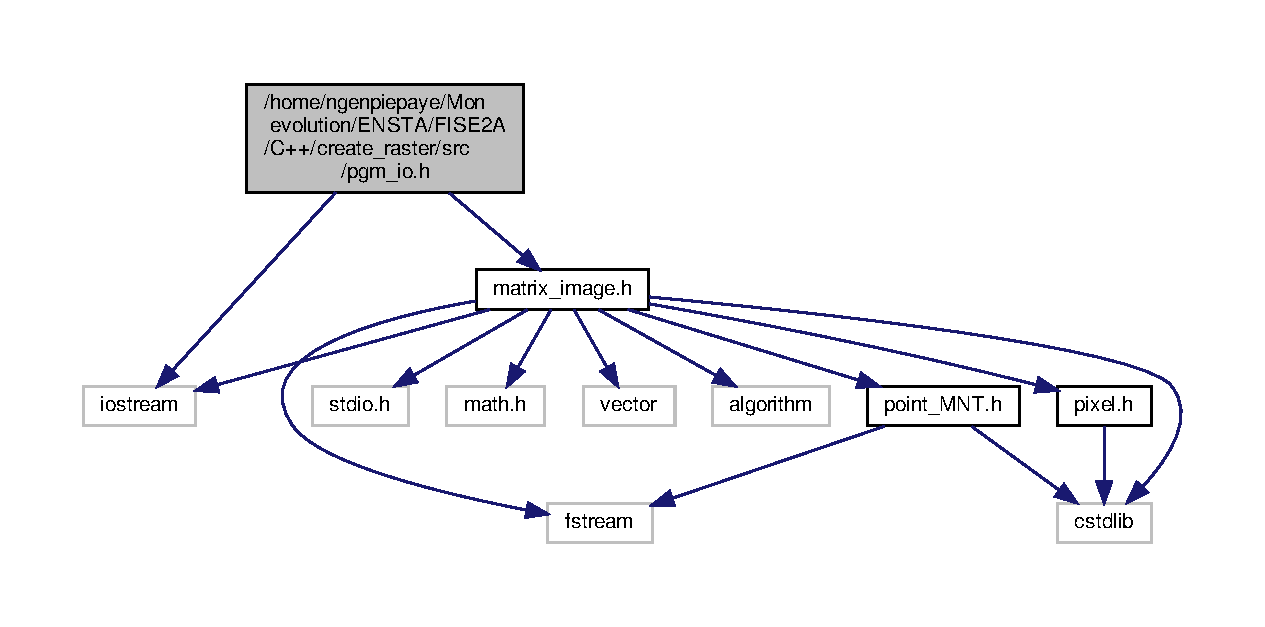
\includegraphics[width=350pt]{pgm__io_8h__incl}
\end{center}
\end{figure}
This graph shows which files directly or indirectly include this file\+:\nopagebreak
\begin{figure}[H]
\begin{center}
\leavevmode
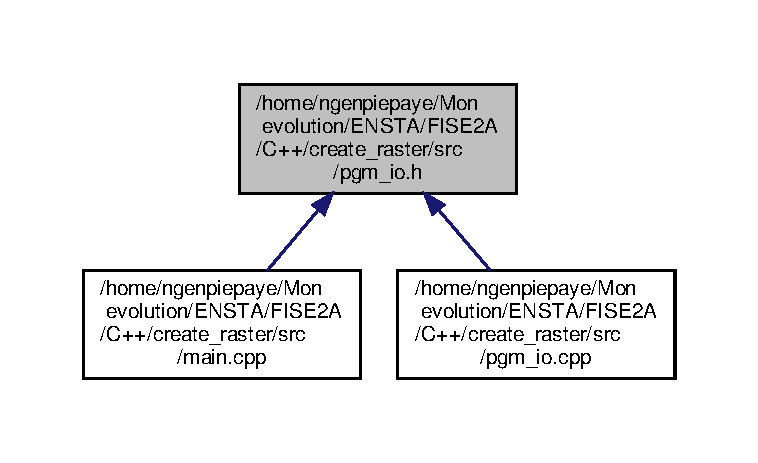
\includegraphics[width=350pt]{pgm__io_8h__dep__incl}
\end{center}
\end{figure}
\subsection*{Functions}
\begin{DoxyCompactItemize}
\item 
void \hyperlink{pgm__io_8h_ab7fa8a14372e30b679e18aaebb431aef}{pgma\+\_\+write} (const string file\+\_\+out\+\_\+name, const \hyperlink{struct_matrix__image}{Matrix\+\_\+image} \&matrix)
\item 
void \hyperlink{pgm__io_8h_a4ae7c77bd527a74fa07a12ce2dab893d}{pgma\+\_\+write\+\_\+data} (ofstream \&file\+\_\+out, const \hyperlink{struct_matrix__image}{Matrix\+\_\+image} \&matrix)
\item 
void \hyperlink{pgm__io_8h_a56d84487bbeb0e07e53438efb73f1dbd}{pgma\+\_\+write\+\_\+header} (ofstream \&file\+\_\+out, const string file\+\_\+out\+\_\+name, const \hyperlink{struct_matrix__image}{Matrix\+\_\+image} \&matrix, const unsigned int maxg)
\item 
void \hyperlink{pgm__io_8h_ae8de00c9a7e3050255f0384756415d4d}{pgmb\+\_\+write} (const string file\+\_\+out\+\_\+name, const \hyperlink{struct_matrix__image}{Matrix\+\_\+image} \&matrix)
\item 
void \hyperlink{pgm__io_8h_a7bfef37ecef81cfe8cabb7b38fa1cc4d}{pgmb\+\_\+write\+\_\+data} (ofstream \&file\+\_\+out, const \hyperlink{struct_matrix__image}{Matrix\+\_\+image} \&matrix)
\item 
void \hyperlink{pgm__io_8h_ad40499194530bfd31e395fd7a65d4c5a}{pgmb\+\_\+write\+\_\+header} (ofstream \&file\+\_\+out, const string file\+\_\+out\+\_\+name, const \hyperlink{struct_matrix__image}{Matrix\+\_\+image} \&matrix, const unsigned int maxg)
\end{DoxyCompactItemize}


\subsection{Function Documentation}
\mbox{\Hypertarget{pgm__io_8h_ab7fa8a14372e30b679e18aaebb431aef}\label{pgm__io_8h_ab7fa8a14372e30b679e18aaebb431aef}} 
\index{pgm\+\_\+io.\+h@{pgm\+\_\+io.\+h}!pgma\+\_\+write@{pgma\+\_\+write}}
\index{pgma\+\_\+write@{pgma\+\_\+write}!pgm\+\_\+io.\+h@{pgm\+\_\+io.\+h}}
\subsubsection{\texorpdfstring{pgma\+\_\+write()}{pgma\_write()}}
{\footnotesize\ttfamily void pgma\+\_\+write (\begin{DoxyParamCaption}\item[{const string}]{output\+\_\+name,  }\item[{const \hyperlink{struct_matrix__image}{Matrix\+\_\+image} \&}]{matrix }\end{DoxyParamCaption})}

~\newline
$\ast$$\ast$$\ast$$\ast$$\ast$$\ast$$\ast$$\ast$$\ast$$\ast$$\ast$$\ast$$\ast$$\ast$$\ast$$\ast$$\ast$$\ast$$\ast$$\ast$$\ast$$\ast$$\ast$$\ast$$\ast$$\ast$$\ast$$\ast$$\ast$$\ast$$\ast$$\ast$$\ast$$\ast$$\ast$$\ast$$\ast$$\ast$$\ast$$\ast$$\ast$$\ast$$\ast$$\ast$$\ast$$\ast$$\ast$$\ast$$\ast$$\ast$$\ast$$\ast$$\ast$$\ast$$\ast$$\ast$$\ast$$\ast$$\ast$$\ast$$\ast$$\ast$$\ast$$\ast$$\ast$$\ast$$\ast$$\ast$$\ast$$\ast$$\ast$$\ast$$\ast$$\ast$$\ast$$\ast$~\newline
\textbackslash{} ~\newline
\textbackslash{} Purpose\+:~\newline
\textbackslash{} ~\newline
\textbackslash{} P\+G\+M\+A\+\_\+\+W\+R\+I\+TE writes the header and data for an A\+S\+C\+II P\+GM file.~\newline
\textbackslash{} ~\newline
\textbackslash{} Example\+:~\newline
\textbackslash{} ~\newline
\textbackslash{} P2~\newline
\textbackslash{} \# feep.\+pgm~\newline
\textbackslash{} 24 7~\newline
\textbackslash{} 15~\newline
\textbackslash{} 0 0 0 0 0 0 0 0 0 0 0 0 0 0 0 0 0 0 0 0 0 0 0 0~\newline
\textbackslash{} 0 3 3 3 3 0 0 7 7 7 7 0 0 11 11 11 11 0 0 15 15 15 15 0~\newline
\textbackslash{} 0 3 0 0 0 0 0 7 0 0 0 0 0 11 0 0 0 0 0 15 0 0 15 0~\newline
\textbackslash{} 0 3 3 3 0 0 0 7 7 7 0 0 0 11 11 11 0 0 0 15 15 15 15 0~\newline
\textbackslash{} 0 3 0 0 0 0 0 7 0 0 0 0 0 11 0 0 0 0 0 15 0 0 0 0~\newline
\textbackslash{} 0 3 0 0 0 0 0 7 7 7 7 0 0 11 11 11 11 0 0 15 0 0 0 0~\newline
\textbackslash{} 0 0 0 0 0 0 0 0 0 0 0 0 0 0 0 0 0 0 0 0 0 0 0 0~\newline
\textbackslash{} ~\newline
\textbackslash{} Author\+:~\newline
\textbackslash{} ~\newline
\textbackslash{} stephane N\+G\+N\+E\+P\+I\+E\+P\+A\+YE W\+E\+M\+BE~\newline
\textbackslash{} ~\newline
\textbackslash{} Parameters\+:~\newline
\textbackslash{} ~\newline
\textbackslash{} Input, string O\+U\+T\+P\+U\+T\+\_\+\+N\+A\+ME, the name of the file.~\newline
\textbackslash{} ~\newline
\textbackslash{} Input, \hyperlink{struct_matrix__image}{Matrix\+\_\+image}\& matrix matrix of pixel.~\newline
\textbackslash{} ~\newline


Definition at line 12 of file pgm\+\_\+io.\+cpp.

\mbox{\Hypertarget{pgm__io_8h_a4ae7c77bd527a74fa07a12ce2dab893d}\label{pgm__io_8h_a4ae7c77bd527a74fa07a12ce2dab893d}} 
\index{pgm\+\_\+io.\+h@{pgm\+\_\+io.\+h}!pgma\+\_\+write\+\_\+data@{pgma\+\_\+write\+\_\+data}}
\index{pgma\+\_\+write\+\_\+data@{pgma\+\_\+write\+\_\+data}!pgm\+\_\+io.\+h@{pgm\+\_\+io.\+h}}
\subsubsection{\texorpdfstring{pgma\+\_\+write\+\_\+data()}{pgma\_write\_data()}}
{\footnotesize\ttfamily void pgma\+\_\+write\+\_\+data (\begin{DoxyParamCaption}\item[{ofstream \&}]{output,  }\item[{const \hyperlink{struct_matrix__image}{Matrix\+\_\+image} \&}]{matrix }\end{DoxyParamCaption})}

~\newline
$\ast$$\ast$$\ast$$\ast$$\ast$$\ast$$\ast$$\ast$$\ast$$\ast$$\ast$$\ast$$\ast$$\ast$$\ast$$\ast$$\ast$$\ast$$\ast$$\ast$$\ast$$\ast$$\ast$$\ast$$\ast$$\ast$$\ast$$\ast$$\ast$$\ast$$\ast$$\ast$$\ast$$\ast$$\ast$$\ast$$\ast$$\ast$$\ast$$\ast$$\ast$$\ast$$\ast$$\ast$$\ast$$\ast$$\ast$$\ast$$\ast$$\ast$$\ast$$\ast$$\ast$$\ast$$\ast$$\ast$$\ast$$\ast$$\ast$$\ast$$\ast$$\ast$$\ast$$\ast$$\ast$$\ast$$\ast$$\ast$$\ast$$\ast$$\ast$$\ast$$\ast$$\ast$$\ast$$\ast$~\newline
\textbackslash{} ~\newline
\textbackslash{} Purpose\+:~\newline
\textbackslash{} ~\newline
\textbackslash{} P\+G\+M\+A\+\_\+\+W\+R\+I\+T\+E\+\_\+\+D\+A\+TA writes the data for an A\+S\+C\+II P\+GM file.~\newline
\textbackslash{} ~\newline
\textbackslash{} Author\+:~\newline
\textbackslash{} ~\newline
\textbackslash{} Stephane N\+G\+N\+E\+P\+I\+E\+P\+A\+YE W\+E\+M\+BE~\newline
\textbackslash{} ~\newline
\textbackslash{} Parameters\+:~\newline
\textbackslash{} ~\newline
\textbackslash{} Input, ofstream \&O\+U\+T\+P\+UT, a pointer to the file.~\newline
\textbackslash{} ~\newline
\textbackslash{} Input, \hyperlink{struct_matrix__image}{Matrix\+\_\+image}\& matrix matrix of pixel.~\newline
\textbackslash{} ~\newline


Definition at line 97 of file pgm\+\_\+io.\+cpp.

\mbox{\Hypertarget{pgm__io_8h_a56d84487bbeb0e07e53438efb73f1dbd}\label{pgm__io_8h_a56d84487bbeb0e07e53438efb73f1dbd}} 
\index{pgm\+\_\+io.\+h@{pgm\+\_\+io.\+h}!pgma\+\_\+write\+\_\+header@{pgma\+\_\+write\+\_\+header}}
\index{pgma\+\_\+write\+\_\+header@{pgma\+\_\+write\+\_\+header}!pgm\+\_\+io.\+h@{pgm\+\_\+io.\+h}}
\subsubsection{\texorpdfstring{pgma\+\_\+write\+\_\+header()}{pgma\_write\_header()}}
{\footnotesize\ttfamily void pgma\+\_\+write\+\_\+header (\begin{DoxyParamCaption}\item[{ofstream \&}]{output,  }\item[{const string}]{output\+\_\+name,  }\item[{const \hyperlink{struct_matrix__image}{Matrix\+\_\+image} \&}]{matrix,  }\item[{const unsigned int}]{maxg }\end{DoxyParamCaption})}

~\newline
$\ast$$\ast$$\ast$$\ast$$\ast$$\ast$$\ast$$\ast$$\ast$$\ast$$\ast$$\ast$$\ast$$\ast$$\ast$$\ast$$\ast$$\ast$$\ast$$\ast$$\ast$$\ast$$\ast$$\ast$$\ast$$\ast$$\ast$$\ast$$\ast$$\ast$$\ast$$\ast$$\ast$$\ast$$\ast$$\ast$$\ast$$\ast$$\ast$$\ast$$\ast$$\ast$$\ast$$\ast$$\ast$$\ast$$\ast$$\ast$$\ast$$\ast$$\ast$$\ast$$\ast$$\ast$$\ast$$\ast$$\ast$$\ast$$\ast$$\ast$$\ast$$\ast$$\ast$$\ast$$\ast$$\ast$$\ast$$\ast$$\ast$$\ast$$\ast$$\ast$$\ast$$\ast$$\ast$$\ast$~\newline
\textbackslash{} ~\newline
\textbackslash{} Purpose\+:~\newline
\textbackslash{} ~\newline
\textbackslash{} P\+G\+M\+A\+\_\+\+W\+R\+I\+T\+E\+\_\+\+H\+E\+A\+D\+ER writes the header of an A\+S\+C\+II P\+GM file.~\newline
\textbackslash{} ~\newline
\textbackslash{} Author\+:~\newline
\textbackslash{} ~\newline
\textbackslash{} Steĥane N\+G\+N\+E\+P\+I\+E\+P\+A\+YE W\+E\+M\+BE~\newline
\textbackslash{} ~\newline
\textbackslash{} Parameters\+:~\newline
\textbackslash{} ~\newline
\textbackslash{} Input, ofstream \&O\+U\+T\+P\+UT, a pointer to the file.~\newline
\textbackslash{} ~\newline
\textbackslash{} Input, string O\+U\+T\+P\+U\+T\+\_\+\+N\+A\+ME, the name of the file.~\newline
\textbackslash{} ~\newline
\textbackslash{} Input, \hyperlink{struct_matrix__image}{Matrix\+\_\+image}\& matrix matrix of pixel.~\newline
\textbackslash{} ~\newline
\textbackslash{} Input, unsigned int M\+A\+XG, the maximum gray value.~\newline
\textbackslash{} ~\newline


Definition at line 147 of file pgm\+\_\+io.\+cpp.

\mbox{\Hypertarget{pgm__io_8h_ae8de00c9a7e3050255f0384756415d4d}\label{pgm__io_8h_ae8de00c9a7e3050255f0384756415d4d}} 
\index{pgm\+\_\+io.\+h@{pgm\+\_\+io.\+h}!pgmb\+\_\+write@{pgmb\+\_\+write}}
\index{pgmb\+\_\+write@{pgmb\+\_\+write}!pgm\+\_\+io.\+h@{pgm\+\_\+io.\+h}}
\subsubsection{\texorpdfstring{pgmb\+\_\+write()}{pgmb\_write()}}
{\footnotesize\ttfamily void pgmb\+\_\+write (\begin{DoxyParamCaption}\item[{const string}]{output\+\_\+name,  }\item[{const \hyperlink{struct_matrix__image}{Matrix\+\_\+image} \&}]{matrix }\end{DoxyParamCaption})}

~\newline
$\ast$$\ast$$\ast$$\ast$$\ast$$\ast$$\ast$$\ast$$\ast$$\ast$$\ast$$\ast$$\ast$$\ast$$\ast$$\ast$$\ast$$\ast$$\ast$$\ast$$\ast$$\ast$$\ast$$\ast$$\ast$$\ast$$\ast$$\ast$$\ast$$\ast$$\ast$$\ast$$\ast$$\ast$$\ast$$\ast$$\ast$$\ast$$\ast$$\ast$$\ast$$\ast$$\ast$$\ast$$\ast$$\ast$$\ast$$\ast$$\ast$$\ast$$\ast$$\ast$$\ast$$\ast$$\ast$$\ast$$\ast$$\ast$$\ast$$\ast$$\ast$$\ast$$\ast$$\ast$$\ast$$\ast$$\ast$$\ast$$\ast$$\ast$$\ast$$\ast$$\ast$$\ast$$\ast$$\ast$~\newline
\textbackslash{} ~\newline
\textbackslash{} Purpose\+:~\newline
\textbackslash{} ~\newline
\textbackslash{} P\+G\+M\+B\+\_\+\+W\+R\+I\+TE writes the header and data for a binary P\+GM file.~\newline
\textbackslash{} ~\newline
\textbackslash{} example~\newline
\textbackslash{} ~\newline
\textbackslash{} P3~\newline
\textbackslash{} \# Le P3 signifie que les couleurs sont en A\+S\+C\+II, et qu\textquotesingle{}elles sont en R\+GB.~\newline
\textbackslash{} \# Par 3 colonnes et 2 lignes \+:~\newline
\textbackslash{} 3 2~\newline
\textbackslash{} \# Ayant 255 pour valeur maximum \+:~\newline
\textbackslash{} data ...~\newline
\textbackslash{} ~\newline
\textbackslash{} Author\+:~\newline
\textbackslash{} ~\newline
\textbackslash{} Stephane N\+G\+N\+E\+P\+I\+E\+P\+A\+YE W\+E\+M\+BE~\newline
\textbackslash{} ~\newline
\textbackslash{} Parameters\+:~\newline
\textbackslash{} ~\newline
\textbackslash{} Input, string O\+U\+T\+P\+U\+T\+\_\+\+N\+A\+ME, the name of the file.~\newline
\textbackslash{} ~\newline
\textbackslash{} Input, \hyperlink{struct_matrix__image}{Matrix\+\_\+image}\& matrix matrix of pixel.~\newline
\textbackslash{} ~\newline


Definition at line 182 of file pgm\+\_\+io.\+cpp.

\mbox{\Hypertarget{pgm__io_8h_a7bfef37ecef81cfe8cabb7b38fa1cc4d}\label{pgm__io_8h_a7bfef37ecef81cfe8cabb7b38fa1cc4d}} 
\index{pgm\+\_\+io.\+h@{pgm\+\_\+io.\+h}!pgmb\+\_\+write\+\_\+data@{pgmb\+\_\+write\+\_\+data}}
\index{pgmb\+\_\+write\+\_\+data@{pgmb\+\_\+write\+\_\+data}!pgm\+\_\+io.\+h@{pgm\+\_\+io.\+h}}
\subsubsection{\texorpdfstring{pgmb\+\_\+write\+\_\+data()}{pgmb\_write\_data()}}
{\footnotesize\ttfamily void pgmb\+\_\+write\+\_\+data (\begin{DoxyParamCaption}\item[{ofstream \&}]{output,  }\item[{const \hyperlink{struct_matrix__image}{Matrix\+\_\+image} \&}]{matrix }\end{DoxyParamCaption})}

~\newline
$\ast$$\ast$$\ast$$\ast$$\ast$$\ast$$\ast$$\ast$$\ast$$\ast$$\ast$$\ast$$\ast$$\ast$$\ast$$\ast$$\ast$$\ast$$\ast$$\ast$$\ast$$\ast$$\ast$$\ast$$\ast$$\ast$$\ast$$\ast$$\ast$$\ast$$\ast$$\ast$$\ast$$\ast$$\ast$$\ast$$\ast$$\ast$$\ast$$\ast$$\ast$$\ast$$\ast$$\ast$$\ast$$\ast$$\ast$$\ast$$\ast$$\ast$$\ast$$\ast$$\ast$$\ast$$\ast$$\ast$$\ast$$\ast$$\ast$$\ast$$\ast$$\ast$$\ast$$\ast$$\ast$$\ast$$\ast$$\ast$$\ast$$\ast$$\ast$$\ast$$\ast$$\ast$$\ast$$\ast$~\newline
\textbackslash{} ~\newline
\textbackslash{} Purpose\+:~\newline
\textbackslash{} ~\newline
\textbackslash{} P\+G\+M\+B\+\_\+\+W\+R\+I\+T\+E\+\_\+\+D\+A\+TA writes the data for a binary P\+GM file.~\newline
\textbackslash{} ~\newline
\textbackslash{} Author\+:~\newline
\textbackslash{} ~\newline
\textbackslash{} Stephane N\+G\+N\+E\+P\+I\+E\+P\+A\+YE W\+E\+M\+BE~\newline
\textbackslash{} ~\newline
\textbackslash{} Parameters\+:~\newline
\textbackslash{} ~\newline
\textbackslash{} Input, ofstream \&O\+U\+T\+P\+UT, a pointer to the file.~\newline
\textbackslash{} ~\newline
\textbackslash{} Input, \hyperlink{struct_matrix__image}{Matrix\+\_\+image}\& matrix matrix of pixel.~\newline
\textbackslash{} ~\newline


Definition at line 262 of file pgm\+\_\+io.\+cpp.

\mbox{\Hypertarget{pgm__io_8h_ad40499194530bfd31e395fd7a65d4c5a}\label{pgm__io_8h_ad40499194530bfd31e395fd7a65d4c5a}} 
\index{pgm\+\_\+io.\+h@{pgm\+\_\+io.\+h}!pgmb\+\_\+write\+\_\+header@{pgmb\+\_\+write\+\_\+header}}
\index{pgmb\+\_\+write\+\_\+header@{pgmb\+\_\+write\+\_\+header}!pgm\+\_\+io.\+h@{pgm\+\_\+io.\+h}}
\subsubsection{\texorpdfstring{pgmb\+\_\+write\+\_\+header()}{pgmb\_write\_header()}}
{\footnotesize\ttfamily void pgmb\+\_\+write\+\_\+header (\begin{DoxyParamCaption}\item[{ofstream \&}]{output,  }\item[{const string}]{output\+\_\+name,  }\item[{const \hyperlink{struct_matrix__image}{Matrix\+\_\+image} \&}]{matrix,  }\item[{const unsigned int}]{maxg }\end{DoxyParamCaption})}

~\newline
$\ast$$\ast$$\ast$$\ast$$\ast$$\ast$$\ast$$\ast$$\ast$$\ast$$\ast$$\ast$$\ast$$\ast$$\ast$$\ast$$\ast$$\ast$$\ast$$\ast$$\ast$$\ast$$\ast$$\ast$$\ast$$\ast$$\ast$$\ast$$\ast$$\ast$$\ast$$\ast$$\ast$$\ast$$\ast$$\ast$$\ast$$\ast$$\ast$$\ast$$\ast$$\ast$$\ast$$\ast$$\ast$$\ast$$\ast$$\ast$$\ast$$\ast$$\ast$$\ast$$\ast$$\ast$$\ast$$\ast$$\ast$$\ast$$\ast$$\ast$$\ast$$\ast$$\ast$$\ast$$\ast$$\ast$$\ast$$\ast$$\ast$$\ast$$\ast$$\ast$$\ast$$\ast$$\ast$$\ast$80~\newline
\textbackslash{} ~\newline
\textbackslash{} Purpose\+:~\newline
\textbackslash{} ~\newline
\textbackslash{} P\+G\+M\+B\+\_\+\+W\+R\+I\+T\+E\+\_\+\+H\+E\+A\+D\+ER writes the header of a binary P\+GM file.~\newline
\textbackslash{} ~\newline
\textbackslash{} Author\+:~\newline
\textbackslash{} ~\newline
\textbackslash{} Stephane N\+G\+N\+E\+P\+I\+E\+P\+A\+YE W\+E\+M\+BE~\newline
\textbackslash{} ~\newline
\textbackslash{} Parameters\+:~\newline
\textbackslash{} ~\newline
\textbackslash{} Input, ofstream \&O\+U\+T\+P\+UT, a pointer to the file.~\newline
\textbackslash{} ~\newline
\textbackslash{} Input, string O\+U\+T\+P\+U\+T\+\_\+\+N\+A\+ME, the name of the file.~\newline
\textbackslash{} ~\newline
\textbackslash{} Input, \hyperlink{struct_matrix__image}{Matrix\+\_\+image}\& matrix matrix of pixel.~\newline
\textbackslash{} ~\newline
\textbackslash{} Input, unsigned int M\+A\+XG, the maximum gray value.~\newline
\textbackslash{} ~\newline


Definition at line 299 of file pgm\+\_\+io.\+cpp.


\hypertarget{pixel_8cpp}{}\section{/home/ngenpiepaye/\+Mon evolution/\+E\+N\+S\+T\+A/\+F\+I\+S\+E2\+A/\+C++/create\+\_\+raster/src/pixel.cpp File Reference}
\label{pixel_8cpp}\index{/home/ngenpiepaye/\+Mon evolution/\+E\+N\+S\+T\+A/\+F\+I\+S\+E2\+A/\+C++/create\+\_\+raster/src/pixel.\+cpp@{/home/ngenpiepaye/\+Mon evolution/\+E\+N\+S\+T\+A/\+F\+I\+S\+E2\+A/\+C++/create\+\_\+raster/src/pixel.\+cpp}}
{\ttfamily \#include \char`\"{}pixel.\+h\char`\"{}}\newline
{\ttfamily \#include $<$iostream$>$}\newline
{\ttfamily \#include $<$math.\+h$>$}\newline
Include dependency graph for pixel.\+cpp\+:\nopagebreak
\begin{figure}[H]
\begin{center}
\leavevmode
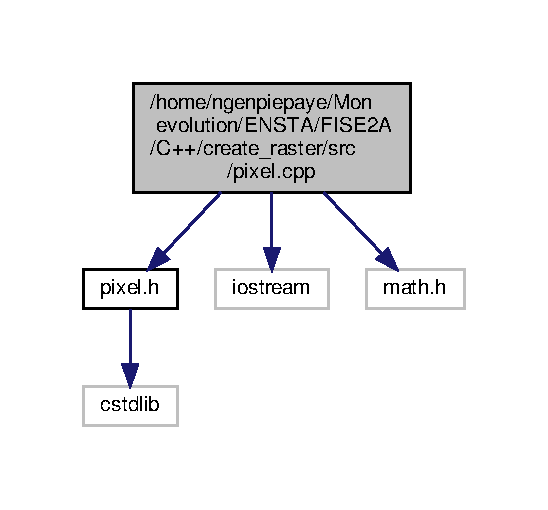
\includegraphics[width=263pt]{pixel_8cpp__incl}
\end{center}
\end{figure}

\hypertarget{pixel_8h}{}\section{/home/ngenpiepaye/\+Mon evolution/\+E\+N\+S\+T\+A/\+F\+I\+S\+E2\+A/\+C++/create\+\_\+raster/src/pixel.h File Reference}
\label{pixel_8h}\index{/home/ngenpiepaye/\+Mon evolution/\+E\+N\+S\+T\+A/\+F\+I\+S\+E2\+A/\+C++/create\+\_\+raster/src/pixel.\+h@{/home/ngenpiepaye/\+Mon evolution/\+E\+N\+S\+T\+A/\+F\+I\+S\+E2\+A/\+C++/create\+\_\+raster/src/pixel.\+h}}
{\ttfamily \#include $<$cstdlib$>$}\newline
Include dependency graph for pixel.\+h\+:\nopagebreak
\begin{figure}[H]
\begin{center}
\leavevmode
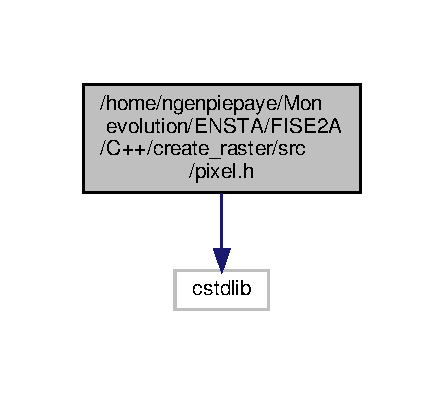
\includegraphics[width=213pt]{pixel_8h__incl}
\end{center}
\end{figure}
This graph shows which files directly or indirectly include this file\+:\nopagebreak
\begin{figure}[H]
\begin{center}
\leavevmode
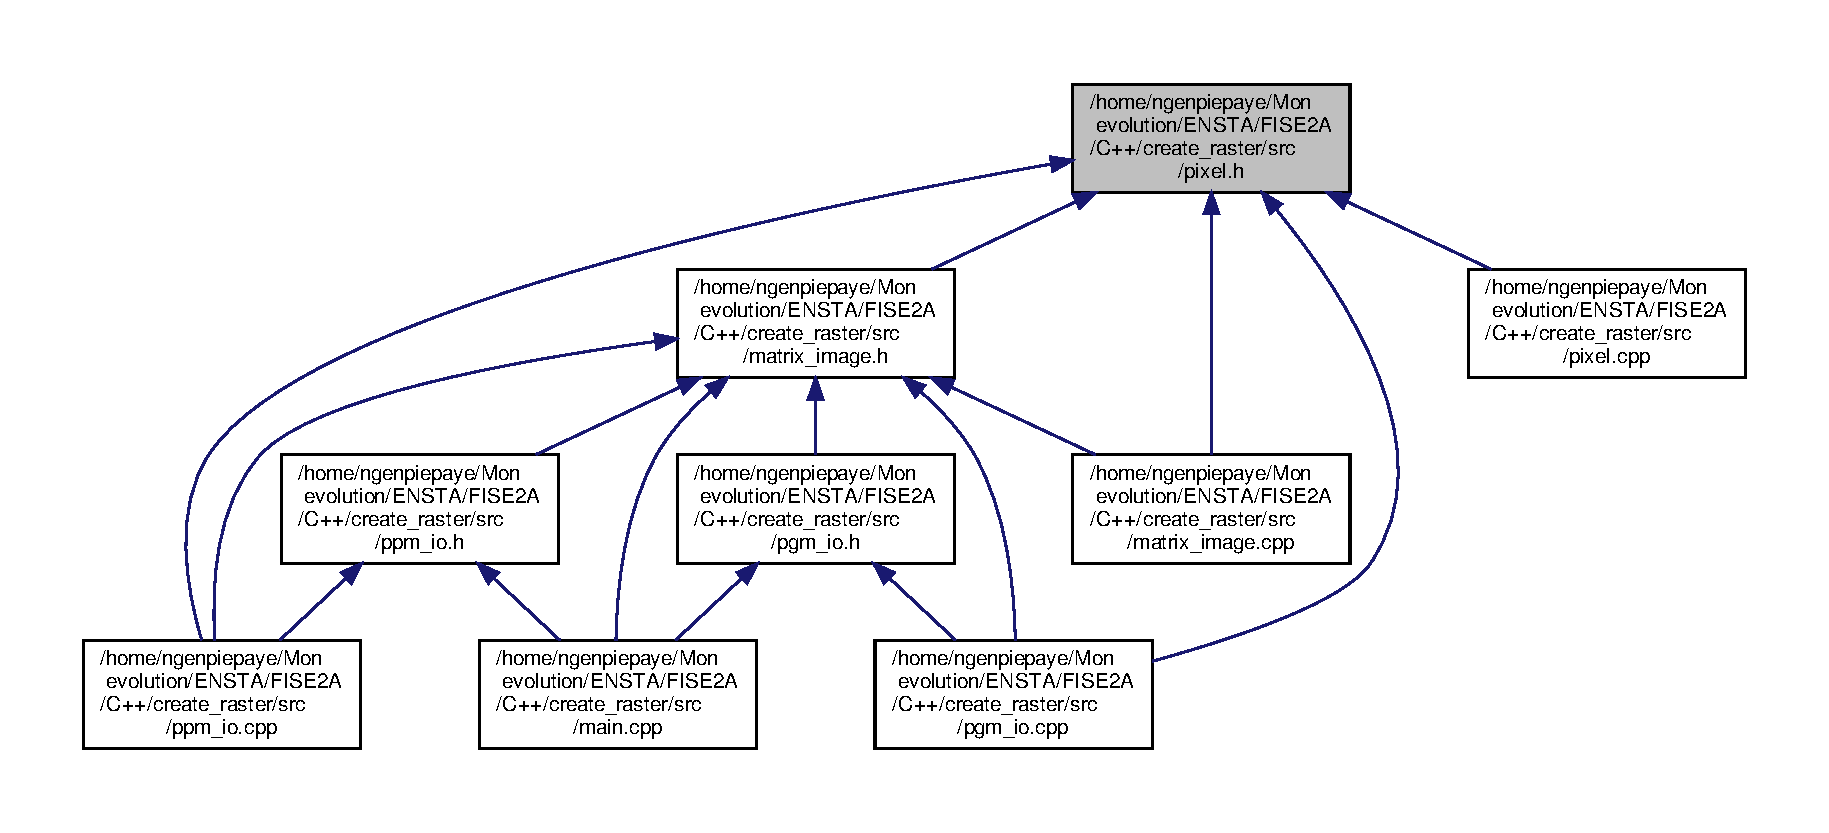
\includegraphics[width=350pt]{pixel_8h__dep__incl}
\end{center}
\end{figure}
\subsection*{Classes}
\begin{DoxyCompactItemize}
\item 
class \hyperlink{class_pixel}{Pixel}
\end{DoxyCompactItemize}
\subsection*{Macros}
\begin{DoxyCompactItemize}
\item 
\#define \hyperlink{pixel_8h_ae71449b1cc6e6250b91f539153a7a0d3}{M\+\_\+\+PI}~3.\+14159265358979323846
\end{DoxyCompactItemize}


\subsection{Macro Definition Documentation}
\mbox{\Hypertarget{pixel_8h_ae71449b1cc6e6250b91f539153a7a0d3}\label{pixel_8h_ae71449b1cc6e6250b91f539153a7a0d3}} 
\index{pixel.\+h@{pixel.\+h}!M\+\_\+\+PI@{M\+\_\+\+PI}}
\index{M\+\_\+\+PI@{M\+\_\+\+PI}!pixel.\+h@{pixel.\+h}}
\subsubsection{\texorpdfstring{M\+\_\+\+PI}{M\_PI}}
{\footnotesize\ttfamily \#define M\+\_\+\+PI~3.\+14159265358979323846}



Definition at line 5 of file pixel.\+h.


\hypertarget{point___m_n_t_8cpp}{}\section{/home/ngenpiepaye/\+Mon evolution/\+E\+N\+S\+T\+A/\+F\+I\+S\+E2\+A/\+C++/create\+\_\+raster/src/point\+\_\+\+M\+NT.cpp File Reference}
\label{point___m_n_t_8cpp}\index{/home/ngenpiepaye/\+Mon evolution/\+E\+N\+S\+T\+A/\+F\+I\+S\+E2\+A/\+C++/create\+\_\+raster/src/point\+\_\+\+M\+N\+T.\+cpp@{/home/ngenpiepaye/\+Mon evolution/\+E\+N\+S\+T\+A/\+F\+I\+S\+E2\+A/\+C++/create\+\_\+raster/src/point\+\_\+\+M\+N\+T.\+cpp}}
{\ttfamily \#include \char`\"{}point\+\_\+\+M\+N\+T.\+h\char`\"{}}\newline
{\ttfamily \#include $<$iostream$>$}\newline
Include dependency graph for point\+\_\+\+M\+N\+T.\+cpp\+:\nopagebreak
\begin{figure}[H]
\begin{center}
\leavevmode
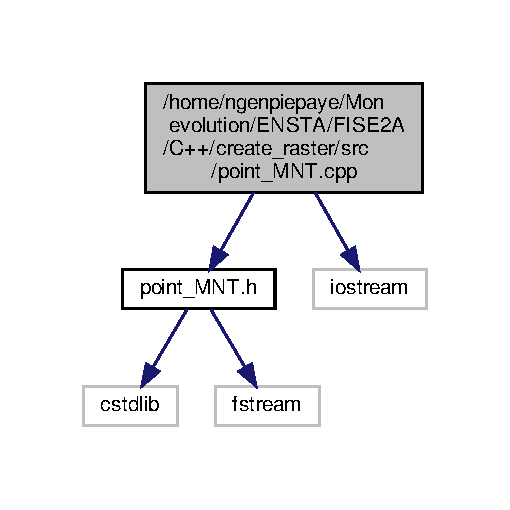
\includegraphics[width=245pt]{point___m_n_t_8cpp__incl}
\end{center}
\end{figure}
\subsection*{Functions}
\begin{DoxyCompactItemize}
\item 
istream \& \hyperlink{point___m_n_t_8cpp_ada8acc622fcfb8d54c76898256fad3aa}{operator$>$$>$} (std\+::istream \&stream, \hyperlink{class_point}{Point} \&p)
\end{DoxyCompactItemize}


\subsection{Function Documentation}
\mbox{\Hypertarget{point___m_n_t_8cpp_ada8acc622fcfb8d54c76898256fad3aa}\label{point___m_n_t_8cpp_ada8acc622fcfb8d54c76898256fad3aa}} 
\index{point\+\_\+\+M\+N\+T.\+cpp@{point\+\_\+\+M\+N\+T.\+cpp}!operator$>$$>$@{operator$>$$>$}}
\index{operator$>$$>$@{operator$>$$>$}!point\+\_\+\+M\+N\+T.\+cpp@{point\+\_\+\+M\+N\+T.\+cpp}}
\subsubsection{\texorpdfstring{operator$>$$>$()}{operator>>()}}
{\footnotesize\ttfamily istream\& operator$>$$>$ (\begin{DoxyParamCaption}\item[{std\+::istream \&}]{stream,  }\item[{\hyperlink{class_point}{Point} \&}]{p }\end{DoxyParamCaption})}

~\newline
$\ast$$\ast$$\ast$$\ast$$\ast$$\ast$$\ast$$\ast$$\ast$$\ast$$\ast$$\ast$$\ast$$\ast$$\ast$$\ast$$\ast$$\ast$$\ast$$\ast$$\ast$$\ast$$\ast$$\ast$$\ast$$\ast$$\ast$$\ast$$\ast$$\ast$$\ast$$\ast$$\ast$$\ast$$\ast$$\ast$$\ast$$\ast$$\ast$$\ast$$\ast$$\ast$$\ast$$\ast$$\ast$$\ast$$\ast$$\ast$$\ast$$\ast$$\ast$$\ast$$\ast$$\ast$$\ast$$\ast$$\ast$$\ast$$\ast$$\ast$$\ast$$\ast$$\ast$$\ast$$\ast$$\ast$$\ast$$\ast$$\ast$$\ast$$\ast$$\ast$$\ast$$\ast$$\ast$$\ast$~\newline
\textbackslash{} ~\newline
\textbackslash{} Purpose\+:~\newline
\textbackslash{} ~\newline
\textbackslash{} surcharge de l\textquotesingle{}operateur de lecture~\newline
\textbackslash{} ~\newline
\textbackslash{} Author\+:~\newline
\textbackslash{} ~\newline
\textbackslash{} stephane N\+G\+N\+E\+P\+I\+E\+P\+A\+YE W\+E\+M\+BE~\newline
\textbackslash{} ~\newline
\textbackslash{} Parameters\+:~\newline
\textbackslash{} ~\newline
\textbackslash{} Input, std\+::istream\& stream, a pointer to the file.~\newline
\textbackslash{} ~\newline
\textbackslash{} Input, \hyperlink{class_point}{Point}\& p, point which will containt the reading data.~\newline
\textbackslash{} ~\newline


Definition at line 58 of file point\+\_\+\+M\+N\+T.\+cpp.


\hypertarget{point___m_n_t_8h}{}\section{/home/ngenpiepaye/\+Mon evolution/\+E\+N\+S\+T\+A/\+F\+I\+S\+E2\+A/\+C++/create\+\_\+raster/src/point\+\_\+\+M\+NT.h File Reference}
\label{point___m_n_t_8h}\index{/home/ngenpiepaye/\+Mon evolution/\+E\+N\+S\+T\+A/\+F\+I\+S\+E2\+A/\+C++/create\+\_\+raster/src/point\+\_\+\+M\+N\+T.\+h@{/home/ngenpiepaye/\+Mon evolution/\+E\+N\+S\+T\+A/\+F\+I\+S\+E2\+A/\+C++/create\+\_\+raster/src/point\+\_\+\+M\+N\+T.\+h}}
{\ttfamily \#include $<$cstdlib$>$}\newline
{\ttfamily \#include $<$fstream$>$}\newline
Include dependency graph for point\+\_\+\+M\+N\+T.\+h\+:\nopagebreak
\begin{figure}[H]
\begin{center}
\leavevmode
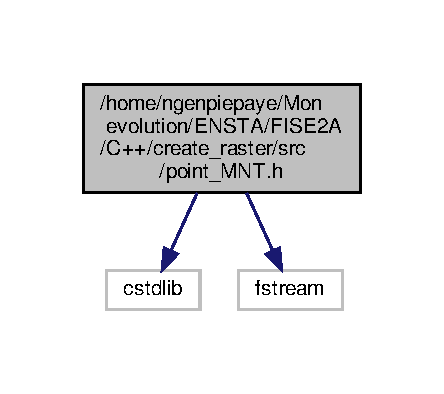
\includegraphics[width=213pt]{point___m_n_t_8h__incl}
\end{center}
\end{figure}
This graph shows which files directly or indirectly include this file\+:\nopagebreak
\begin{figure}[H]
\begin{center}
\leavevmode
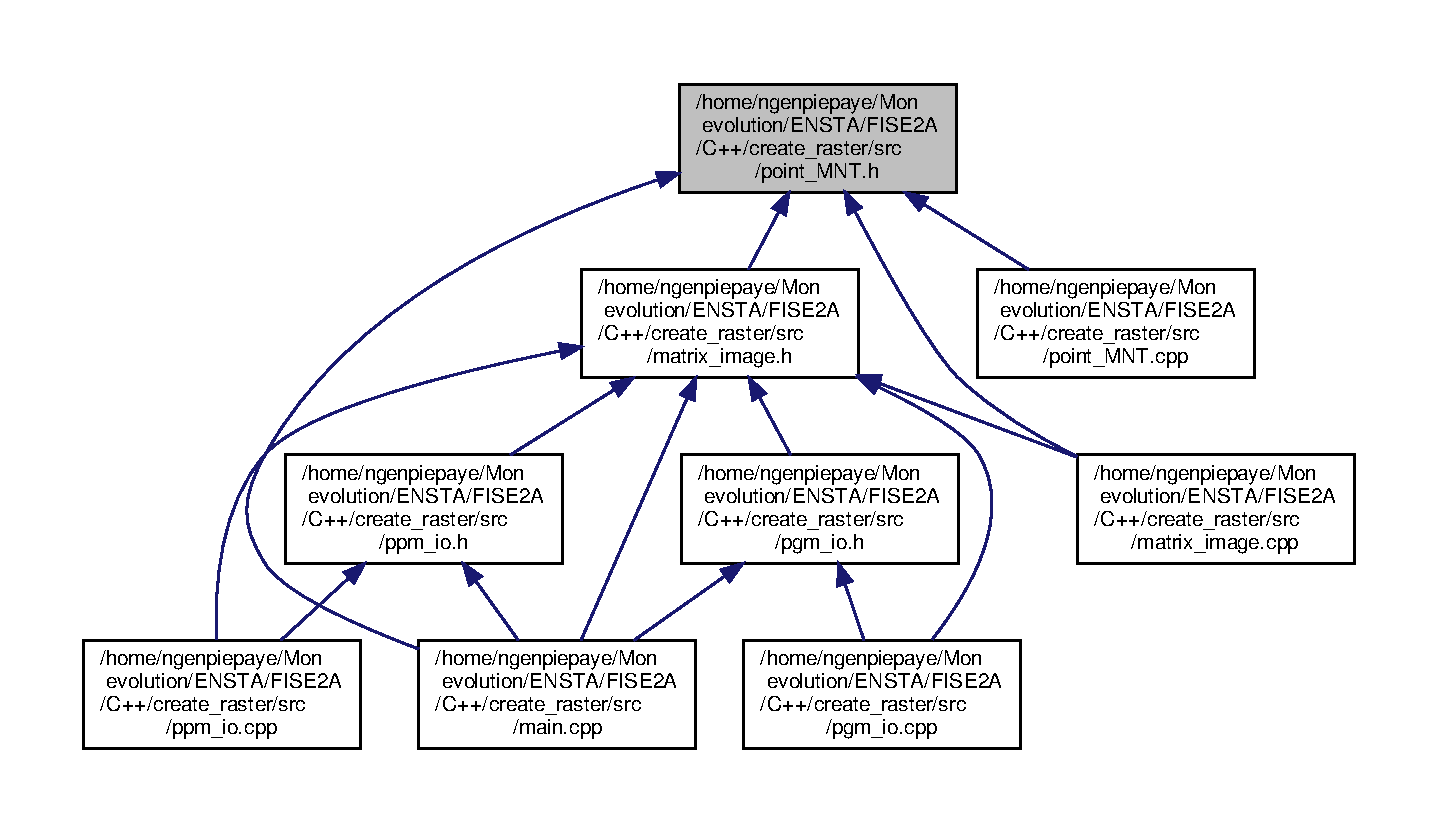
\includegraphics[width=350pt]{point___m_n_t_8h__dep__incl}
\end{center}
\end{figure}
\subsection*{Classes}
\begin{DoxyCompactItemize}
\item 
class \hyperlink{class_point}{Point}
\end{DoxyCompactItemize}

\hypertarget{ppm__io_8cpp}{}\section{/home/ngenpiepaye/\+Mon evolution/\+E\+N\+S\+T\+A/\+F\+I\+S\+E2\+A/\+C++/create\+\_\+raster/src/ppm\+\_\+io.cpp File Reference}
\label{ppm__io_8cpp}\index{/home/ngenpiepaye/\+Mon evolution/\+E\+N\+S\+T\+A/\+F\+I\+S\+E2\+A/\+C++/create\+\_\+raster/src/ppm\+\_\+io.\+cpp@{/home/ngenpiepaye/\+Mon evolution/\+E\+N\+S\+T\+A/\+F\+I\+S\+E2\+A/\+C++/create\+\_\+raster/src/ppm\+\_\+io.\+cpp}}
{\ttfamily \#include $<$cstdlib$>$}\newline
{\ttfamily \#include $<$iostream$>$}\newline
{\ttfamily \#include \char`\"{}matrix\+\_\+image.\+h\char`\"{}}\newline
{\ttfamily \#include \char`\"{}pixel.\+h\char`\"{}}\newline
{\ttfamily \#include \char`\"{}ppm\+\_\+io.\+h\char`\"{}}\newline
Include dependency graph for ppm\+\_\+io.\+cpp\+:\nopagebreak
\begin{figure}[H]
\begin{center}
\leavevmode
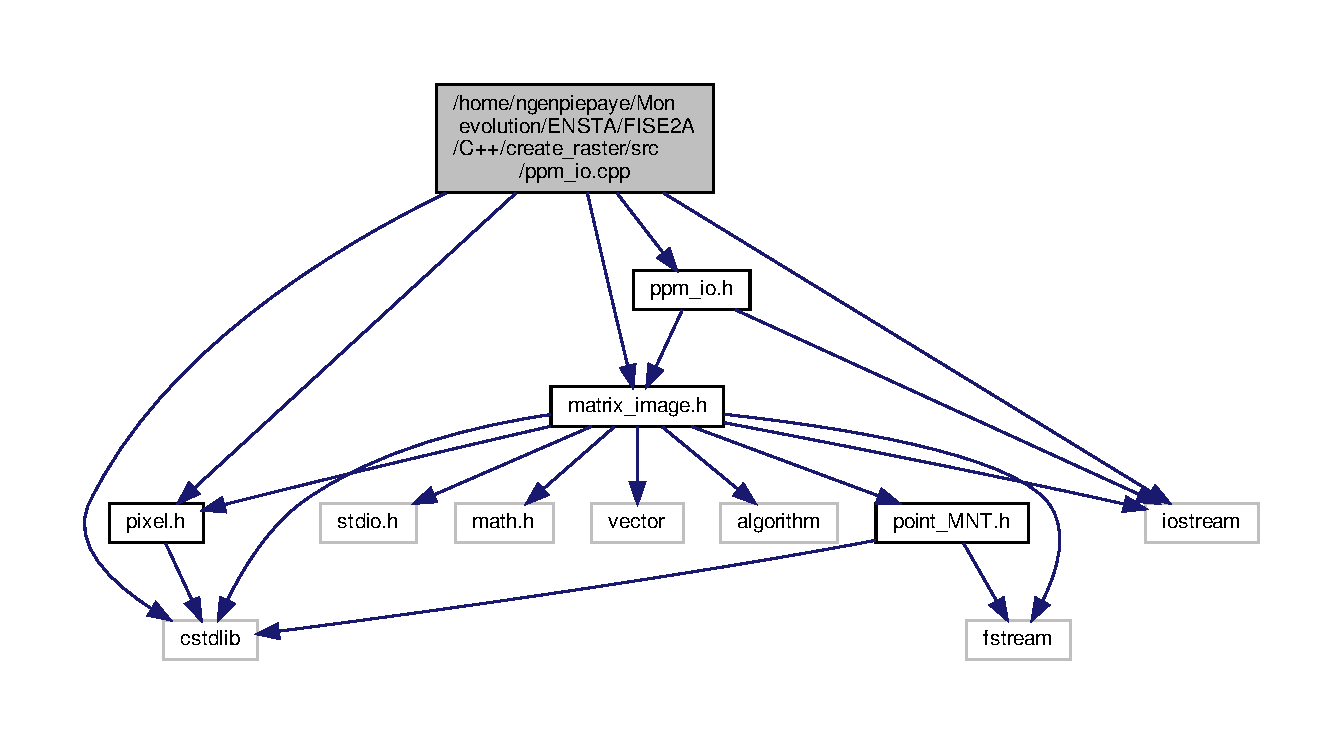
\includegraphics[width=350pt]{ppm__io_8cpp__incl}
\end{center}
\end{figure}
\subsection*{Functions}
\begin{DoxyCompactItemize}
\item 
void \hyperlink{ppm__io_8cpp_a2dad18b70b0d03c91f5969aab5ce92e0}{ppma\+\_\+write} (const string output\+\_\+name, const \hyperlink{struct_matrix__image}{Matrix\+\_\+image} \&matrix)
\item 
void \hyperlink{ppm__io_8cpp_acfbbbe9b9fccd202a02b6baca1d4066e}{ppma\+\_\+write\+\_\+data} (ofstream \&output, const \hyperlink{struct_matrix__image}{Matrix\+\_\+image} \&matrix)
\item 
void \hyperlink{ppm__io_8cpp_aed329f1d22eabf568a36e4c8fcbb2b5f}{ppma\+\_\+write\+\_\+header} (ofstream \&output, const string output\+\_\+name, const \hyperlink{struct_matrix__image}{Matrix\+\_\+image} \&matrix, const unsigned int maxg)
\item 
void \hyperlink{ppm__io_8cpp_a66a427a932e758b96d5e55dc907fd2b7}{ppmb\+\_\+write} (string output\+\_\+name, const \hyperlink{struct_matrix__image}{Matrix\+\_\+image} \&matrix)
\item 
void \hyperlink{ppm__io_8cpp_a34a8e1e588b85119e2819f84dabc8b34}{ppmb\+\_\+write\+\_\+data} (ofstream \&output, const \hyperlink{struct_matrix__image}{Matrix\+\_\+image} \&matrix)
\item 
void \hyperlink{ppm__io_8cpp_a314ed6db5149a13e061270c4c07d9d99}{ppmb\+\_\+write\+\_\+header} (ofstream \&output, const string output\+\_\+name, const \hyperlink{struct_matrix__image}{Matrix\+\_\+image} \&matrix, const unsigned int maxg)
\end{DoxyCompactItemize}


\subsection{Function Documentation}
\mbox{\Hypertarget{ppm__io_8cpp_a2dad18b70b0d03c91f5969aab5ce92e0}\label{ppm__io_8cpp_a2dad18b70b0d03c91f5969aab5ce92e0}} 
\index{ppm\+\_\+io.\+cpp@{ppm\+\_\+io.\+cpp}!ppma\+\_\+write@{ppma\+\_\+write}}
\index{ppma\+\_\+write@{ppma\+\_\+write}!ppm\+\_\+io.\+cpp@{ppm\+\_\+io.\+cpp}}
\subsubsection{\texorpdfstring{ppma\+\_\+write()}{ppma\_write()}}
{\footnotesize\ttfamily void ppma\+\_\+write (\begin{DoxyParamCaption}\item[{const string}]{output\+\_\+name,  }\item[{const \hyperlink{struct_matrix__image}{Matrix\+\_\+image} \&}]{matrix }\end{DoxyParamCaption})}

~\newline
$\ast$$\ast$$\ast$$\ast$$\ast$$\ast$$\ast$$\ast$$\ast$$\ast$$\ast$$\ast$$\ast$$\ast$$\ast$$\ast$$\ast$$\ast$$\ast$$\ast$$\ast$$\ast$$\ast$$\ast$$\ast$$\ast$$\ast$$\ast$$\ast$$\ast$$\ast$$\ast$$\ast$$\ast$$\ast$$\ast$$\ast$$\ast$$\ast$$\ast$$\ast$$\ast$$\ast$$\ast$$\ast$$\ast$$\ast$$\ast$$\ast$$\ast$$\ast$$\ast$$\ast$$\ast$$\ast$$\ast$$\ast$$\ast$$\ast$$\ast$$\ast$$\ast$$\ast$$\ast$$\ast$$\ast$$\ast$$\ast$$\ast$$\ast$$\ast$$\ast$$\ast$$\ast$$\ast$$\ast$~\newline
\textbackslash{} ~\newline
\textbackslash{} Purpose\+:~\newline
\textbackslash{} ~\newline
\textbackslash{} P\+P\+M\+A\+\_\+\+W\+R\+I\+TE writes the header and data for an A\+S\+C\+II P\+PM file.~\newline
\textbackslash{} ~\newline
\textbackslash{} example~\newline
\textbackslash{} ~\newline
\textbackslash{} P3~\newline
\textbackslash{} \# Le P3 signifie que les couleurs sont en A\+S\+C\+II, et qu\textquotesingle{}elles sont en R\+GB.~\newline
\textbackslash{} \# Par 3 colonnes et 2 lignes \+:~\newline
\textbackslash{} 3 2~\newline
\textbackslash{} \# Ayant 255 pour valeur maximum \+:~\newline
\textbackslash{} 255~\newline
\textbackslash{} 255 0 0 ~\newline
\textbackslash{} 0 255 0 ~\newline
 \textbackslash{} 0 0 255~\newline
\textbackslash{} 255 255 0 ~\newline
\textbackslash{} 255 255 255 ~\newline
 \textbackslash{} 0 0 0~\newline
\textbackslash{} ~\newline
\textbackslash{} Author\+:~\newline
\textbackslash{} ~\newline
\textbackslash{} Stephane N\+G\+N\+E\+P\+I\+E\+P\+A\+YE W\+E\+M\+BE~\newline
\textbackslash{} ~\newline
\textbackslash{} Parameters\+:~\newline
\textbackslash{} ~\newline
\textbackslash{} Input, string O\+U\+T\+P\+U\+T\+\_\+\+N\+A\+ME, the name of the file.~\newline
\textbackslash{} ~\newline
\textbackslash{} Input, \hyperlink{struct_matrix__image}{Matrix\+\_\+image}\& matrix matrix of pixel.~\newline
\textbackslash{} ~\newline


Definition at line 12 of file ppm\+\_\+io.\+cpp.

\mbox{\Hypertarget{ppm__io_8cpp_acfbbbe9b9fccd202a02b6baca1d4066e}\label{ppm__io_8cpp_acfbbbe9b9fccd202a02b6baca1d4066e}} 
\index{ppm\+\_\+io.\+cpp@{ppm\+\_\+io.\+cpp}!ppma\+\_\+write\+\_\+data@{ppma\+\_\+write\+\_\+data}}
\index{ppma\+\_\+write\+\_\+data@{ppma\+\_\+write\+\_\+data}!ppm\+\_\+io.\+cpp@{ppm\+\_\+io.\+cpp}}
\subsubsection{\texorpdfstring{ppma\+\_\+write\+\_\+data()}{ppma\_write\_data()}}
{\footnotesize\ttfamily void ppma\+\_\+write\+\_\+data (\begin{DoxyParamCaption}\item[{ofstream \&}]{output,  }\item[{const \hyperlink{struct_matrix__image}{Matrix\+\_\+image} \&}]{matrix }\end{DoxyParamCaption})}

~\newline
$\ast$$\ast$$\ast$$\ast$$\ast$$\ast$$\ast$$\ast$$\ast$$\ast$$\ast$$\ast$$\ast$$\ast$$\ast$$\ast$$\ast$$\ast$$\ast$$\ast$$\ast$$\ast$$\ast$$\ast$$\ast$$\ast$$\ast$$\ast$$\ast$$\ast$$\ast$$\ast$$\ast$$\ast$$\ast$$\ast$$\ast$$\ast$$\ast$$\ast$$\ast$$\ast$$\ast$$\ast$$\ast$$\ast$$\ast$$\ast$$\ast$$\ast$$\ast$$\ast$$\ast$$\ast$$\ast$$\ast$$\ast$$\ast$$\ast$$\ast$$\ast$$\ast$$\ast$$\ast$$\ast$$\ast$$\ast$$\ast$$\ast$$\ast$$\ast$$\ast$$\ast$$\ast$$\ast$$\ast$~\newline
\textbackslash{} ~\newline
\textbackslash{} Purpose\+:~\newline
\textbackslash{} ~\newline
\textbackslash{} P\+P\+M\+A\+\_\+\+W\+R\+I\+T\+E\+\_\+\+D\+A\+TA writes the data for an A\+S\+C\+II P\+PM file.~\newline
\textbackslash{} ~\newline
\textbackslash{} Author\+:~\newline
\textbackslash{} ~\newline
\textbackslash{} Stephane N\+G\+N\+E\+P\+I\+E\+P\+A\+YE W\+E\+M\+BE~\newline
\textbackslash{} ~\newline
\textbackslash{} Parameters\+:~\newline
\textbackslash{} ~\newline
\textbackslash{} Input, ofstream \&O\+U\+T\+P\+UT, a pointer to the file.~\newline
\textbackslash{} ~\newline
\textbackslash{} Input, \hyperlink{struct_matrix__image}{Matrix\+\_\+image}\& matrix matrix of pixel.~\newline
\textbackslash{} ~\newline


Definition at line 98 of file ppm\+\_\+io.\+cpp.

\mbox{\Hypertarget{ppm__io_8cpp_aed329f1d22eabf568a36e4c8fcbb2b5f}\label{ppm__io_8cpp_aed329f1d22eabf568a36e4c8fcbb2b5f}} 
\index{ppm\+\_\+io.\+cpp@{ppm\+\_\+io.\+cpp}!ppma\+\_\+write\+\_\+header@{ppma\+\_\+write\+\_\+header}}
\index{ppma\+\_\+write\+\_\+header@{ppma\+\_\+write\+\_\+header}!ppm\+\_\+io.\+cpp@{ppm\+\_\+io.\+cpp}}
\subsubsection{\texorpdfstring{ppma\+\_\+write\+\_\+header()}{ppma\_write\_header()}}
{\footnotesize\ttfamily void ppma\+\_\+write\+\_\+header (\begin{DoxyParamCaption}\item[{ofstream \&}]{output,  }\item[{const string}]{output\+\_\+name,  }\item[{const \hyperlink{struct_matrix__image}{Matrix\+\_\+image} \&}]{matrix,  }\item[{const unsigned int}]{maxg }\end{DoxyParamCaption})}

~\newline
$\ast$$\ast$$\ast$$\ast$$\ast$$\ast$$\ast$$\ast$$\ast$$\ast$$\ast$$\ast$$\ast$$\ast$$\ast$$\ast$$\ast$$\ast$$\ast$$\ast$$\ast$$\ast$$\ast$$\ast$$\ast$$\ast$$\ast$$\ast$$\ast$$\ast$$\ast$$\ast$$\ast$$\ast$$\ast$$\ast$$\ast$$\ast$$\ast$$\ast$$\ast$$\ast$$\ast$$\ast$$\ast$$\ast$$\ast$$\ast$$\ast$$\ast$$\ast$$\ast$$\ast$$\ast$$\ast$$\ast$$\ast$$\ast$$\ast$$\ast$$\ast$$\ast$$\ast$$\ast$$\ast$$\ast$$\ast$$\ast$$\ast$$\ast$$\ast$$\ast$$\ast$$\ast$$\ast$$\ast$~\newline
\textbackslash{} ~\newline
\textbackslash{} Purpose\+:~\newline
\textbackslash{} ~\newline
\textbackslash{} P\+P\+M\+A\+\_\+\+W\+R\+I\+T\+E\+\_\+\+H\+E\+A\+D\+ER writes the header of an A\+S\+C\+II P\+PM file.~\newline
\textbackslash{} ~\newline
\textbackslash{} Author\+:~\newline
\textbackslash{} ~\newline
\textbackslash{} Stephane N\+G\+N\+E\+P\+I\+E\+P\+A\+YE W\+E\+M\+BE~\newline
\textbackslash{} ~\newline
\textbackslash{} Parameters\+:~\newline
\textbackslash{} ~\newline
\textbackslash{} Input, ofstream \&O\+U\+T\+P\+UT, a pointer to the file.~\newline
\textbackslash{} ~\newline
\textbackslash{} Input, string O\+U\+T\+P\+U\+T\+\_\+\+N\+A\+ME, the name of the file.~\newline
\textbackslash{} ~\newline
\textbackslash{} Input, \hyperlink{struct_matrix__image}{Matrix\+\_\+image}\& matrix matrix of pixel.~\newline
\textbackslash{} ~\newline
\textbackslash{} Input, unsigned int M\+A\+XG, the maximum gray value.~\newline
\textbackslash{} ~\newline


Definition at line 140 of file ppm\+\_\+io.\+cpp.

\mbox{\Hypertarget{ppm__io_8cpp_a66a427a932e758b96d5e55dc907fd2b7}\label{ppm__io_8cpp_a66a427a932e758b96d5e55dc907fd2b7}} 
\index{ppm\+\_\+io.\+cpp@{ppm\+\_\+io.\+cpp}!ppmb\+\_\+write@{ppmb\+\_\+write}}
\index{ppmb\+\_\+write@{ppmb\+\_\+write}!ppm\+\_\+io.\+cpp@{ppm\+\_\+io.\+cpp}}
\subsubsection{\texorpdfstring{ppmb\+\_\+write()}{ppmb\_write()}}
{\footnotesize\ttfamily void ppmb\+\_\+write (\begin{DoxyParamCaption}\item[{string}]{output\+\_\+name,  }\item[{const \hyperlink{struct_matrix__image}{Matrix\+\_\+image} \&}]{matrix }\end{DoxyParamCaption})}

~\newline
$\ast$$\ast$$\ast$$\ast$$\ast$$\ast$$\ast$$\ast$$\ast$$\ast$$\ast$$\ast$$\ast$$\ast$$\ast$$\ast$$\ast$$\ast$$\ast$$\ast$$\ast$$\ast$$\ast$$\ast$$\ast$$\ast$$\ast$$\ast$$\ast$$\ast$$\ast$$\ast$$\ast$$\ast$$\ast$$\ast$$\ast$$\ast$$\ast$$\ast$$\ast$$\ast$$\ast$$\ast$$\ast$$\ast$$\ast$$\ast$$\ast$$\ast$$\ast$$\ast$$\ast$$\ast$$\ast$$\ast$$\ast$$\ast$$\ast$$\ast$$\ast$$\ast$$\ast$$\ast$$\ast$$\ast$$\ast$$\ast$$\ast$$\ast$$\ast$$\ast$$\ast$$\ast$$\ast$$\ast$ ~\newline
\textbackslash{} ~\newline
\textbackslash{} Purpose\+: ~\newline
\textbackslash{} ~\newline
\textbackslash{} P\+P\+M\+B\+\_\+\+W\+R\+I\+TE writes the header and data for a binary P\+PM file. ~\newline
\textbackslash{} ~\newline
\textbackslash{} example ~\newline
\textbackslash{} ~\newline
\textbackslash{} P3 ~\newline
\textbackslash{} \# Le P3 signifie que les couleurs sont en A\+S\+C\+II, et qu\textquotesingle{}elles sont en R\+GB. ~\newline
\textbackslash{} \# Par 3 colonnes et 2 lignes \+: ~\newline
\textbackslash{} 3 2 ~\newline
\textbackslash{} \# Ayant 255 pour valeur maximum \+: ~\newline
\textbackslash{} data ... ~\newline
\textbackslash{} ~\newline
\textbackslash{} Author\+:~\newline
\textbackslash{} ~\newline
\textbackslash{} Stephane N\+G\+N\+E\+P\+I\+E\+P\+A\+YE W\+E\+M\+BE ~\newline
\textbackslash{} ~\newline
\textbackslash{} Parameters\+: ~\newline
\textbackslash{} ~\newline
\textbackslash{} Input, string O\+U\+T\+P\+U\+T\+\_\+\+N\+A\+ME, the name of the file. ~\newline
\textbackslash{} ~\newline
 \textbackslash{} Input, \hyperlink{struct_matrix__image}{Matrix\+\_\+image}\& matrix matrix of pixel. ~\newline
\textbackslash{} ~\newline


Definition at line 175 of file ppm\+\_\+io.\+cpp.

\mbox{\Hypertarget{ppm__io_8cpp_a34a8e1e588b85119e2819f84dabc8b34}\label{ppm__io_8cpp_a34a8e1e588b85119e2819f84dabc8b34}} 
\index{ppm\+\_\+io.\+cpp@{ppm\+\_\+io.\+cpp}!ppmb\+\_\+write\+\_\+data@{ppmb\+\_\+write\+\_\+data}}
\index{ppmb\+\_\+write\+\_\+data@{ppmb\+\_\+write\+\_\+data}!ppm\+\_\+io.\+cpp@{ppm\+\_\+io.\+cpp}}
\subsubsection{\texorpdfstring{ppmb\+\_\+write\+\_\+data()}{ppmb\_write\_data()}}
{\footnotesize\ttfamily void ppmb\+\_\+write\+\_\+data (\begin{DoxyParamCaption}\item[{ofstream \&}]{output,  }\item[{const \hyperlink{struct_matrix__image}{Matrix\+\_\+image} \&}]{matrix }\end{DoxyParamCaption})}

~\newline
$\ast$$\ast$$\ast$$\ast$$\ast$$\ast$$\ast$$\ast$$\ast$$\ast$$\ast$$\ast$$\ast$$\ast$$\ast$$\ast$$\ast$$\ast$$\ast$$\ast$$\ast$$\ast$$\ast$$\ast$$\ast$$\ast$$\ast$$\ast$$\ast$$\ast$$\ast$$\ast$$\ast$$\ast$$\ast$$\ast$$\ast$$\ast$$\ast$$\ast$$\ast$$\ast$$\ast$$\ast$$\ast$$\ast$$\ast$$\ast$$\ast$$\ast$$\ast$$\ast$$\ast$$\ast$$\ast$$\ast$$\ast$$\ast$$\ast$$\ast$$\ast$$\ast$$\ast$$\ast$$\ast$$\ast$$\ast$$\ast$$\ast$$\ast$$\ast$$\ast$$\ast$$\ast$$\ast$$\ast$ ~\newline
\textbackslash{} ~\newline
\textbackslash{} Purpose\+: ~\newline
\textbackslash{} ~\newline
\textbackslash{} P\+P\+M\+B\+\_\+\+W\+R\+I\+T\+E\+\_\+\+D\+A\+TA writes the data for a binary P\+PM file. ~\newline
\textbackslash{} ~\newline
\textbackslash{} Author\+: ~\newline
\textbackslash{} ~\newline
\textbackslash{} Stephane N\+G\+N\+E\+P\+I\+E\+P\+A\+YE W\+E\+M\+BE ~\newline
\textbackslash{} ~\newline
\textbackslash{} Parameters\+: ~\newline
\textbackslash{} ~\newline
\textbackslash{} Input, ofstream \&O\+U\+T\+P\+UT, a pointer to the file.~\newline
\textbackslash{} ~\newline
\textbackslash{} Input, \hyperlink{struct_matrix__image}{Matrix\+\_\+image}\& matrix matrix of pixel. ~\newline
 \textbackslash{} ~\newline
 

Definition at line 254 of file ppm\+\_\+io.\+cpp.

\mbox{\Hypertarget{ppm__io_8cpp_a314ed6db5149a13e061270c4c07d9d99}\label{ppm__io_8cpp_a314ed6db5149a13e061270c4c07d9d99}} 
\index{ppm\+\_\+io.\+cpp@{ppm\+\_\+io.\+cpp}!ppmb\+\_\+write\+\_\+header@{ppmb\+\_\+write\+\_\+header}}
\index{ppmb\+\_\+write\+\_\+header@{ppmb\+\_\+write\+\_\+header}!ppm\+\_\+io.\+cpp@{ppm\+\_\+io.\+cpp}}
\subsubsection{\texorpdfstring{ppmb\+\_\+write\+\_\+header()}{ppmb\_write\_header()}}
{\footnotesize\ttfamily void ppmb\+\_\+write\+\_\+header (\begin{DoxyParamCaption}\item[{ofstream \&}]{output,  }\item[{const string}]{output\+\_\+name,  }\item[{const \hyperlink{struct_matrix__image}{Matrix\+\_\+image} \&}]{matrix,  }\item[{const unsigned int}]{maxg }\end{DoxyParamCaption})}

~\newline
$\ast$$\ast$$\ast$$\ast$$\ast$$\ast$$\ast$$\ast$$\ast$$\ast$$\ast$$\ast$$\ast$$\ast$$\ast$$\ast$$\ast$$\ast$$\ast$$\ast$$\ast$$\ast$$\ast$$\ast$$\ast$$\ast$$\ast$$\ast$$\ast$$\ast$$\ast$$\ast$$\ast$$\ast$$\ast$$\ast$$\ast$$\ast$$\ast$$\ast$$\ast$$\ast$$\ast$$\ast$$\ast$$\ast$$\ast$$\ast$$\ast$$\ast$$\ast$$\ast$$\ast$$\ast$$\ast$$\ast$$\ast$$\ast$$\ast$$\ast$$\ast$$\ast$$\ast$$\ast$$\ast$$\ast$$\ast$$\ast$$\ast$$\ast$$\ast$$\ast$$\ast$$\ast$$\ast$$\ast$ ~\newline
\textbackslash{} ~\newline
\textbackslash{} Purpose\+: ~\newline
\textbackslash{} ~\newline
\textbackslash{} P\+P\+M\+B\+\_\+\+W\+R\+I\+T\+E\+\_\+\+H\+E\+A\+D\+ER writes the header of a binary P\+PM file. ~\newline
\textbackslash{} ~\newline
\textbackslash{} Author\+: ~\newline
\textbackslash{} ~\newline
\textbackslash{} Stephane N\+G\+N\+E\+P\+I\+E\+P\+A\+YE W\+E\+M\+BE ~\newline
\textbackslash{} ~\newline
\textbackslash{} Parameters\+:~\newline
\textbackslash{} ~\newline
\textbackslash{} Input, ofstream \&O\+U\+T\+P\+UT, a pointer to the file. ~\newline
\textbackslash{} ~\newline
\textbackslash{} Input, string O\+U\+T\+P\+U\+T\+\_\+\+N\+A\+ME, the name of the file.~\newline
\textbackslash{} ~\newline
\textbackslash{} Input, \hyperlink{struct_matrix__image}{Matrix\+\_\+image}\& matrix matrix of pixel. ~\newline
\textbackslash{} ~\newline
\textbackslash{} Input, unsigned int M\+A\+XG, the maximum gray value. ~\newline
\textbackslash{} ~\newline


Definition at line 291 of file ppm\+\_\+io.\+cpp.


\hypertarget{ppm__io_8h}{}\section{/home/ngenpiepaye/\+Mon evolution/\+E\+N\+S\+T\+A/\+F\+I\+S\+E2\+A/\+C++/create\+\_\+raster/src/ppm\+\_\+io.h File Reference}
\label{ppm__io_8h}\index{/home/ngenpiepaye/\+Mon evolution/\+E\+N\+S\+T\+A/\+F\+I\+S\+E2\+A/\+C++/create\+\_\+raster/src/ppm\+\_\+io.\+h@{/home/ngenpiepaye/\+Mon evolution/\+E\+N\+S\+T\+A/\+F\+I\+S\+E2\+A/\+C++/create\+\_\+raster/src/ppm\+\_\+io.\+h}}
{\ttfamily \#include $<$iostream$>$}\newline
{\ttfamily \#include \char`\"{}matrix\+\_\+image.\+h\char`\"{}}\newline
Include dependency graph for ppm\+\_\+io.\+h\+:\nopagebreak
\begin{figure}[H]
\begin{center}
\leavevmode
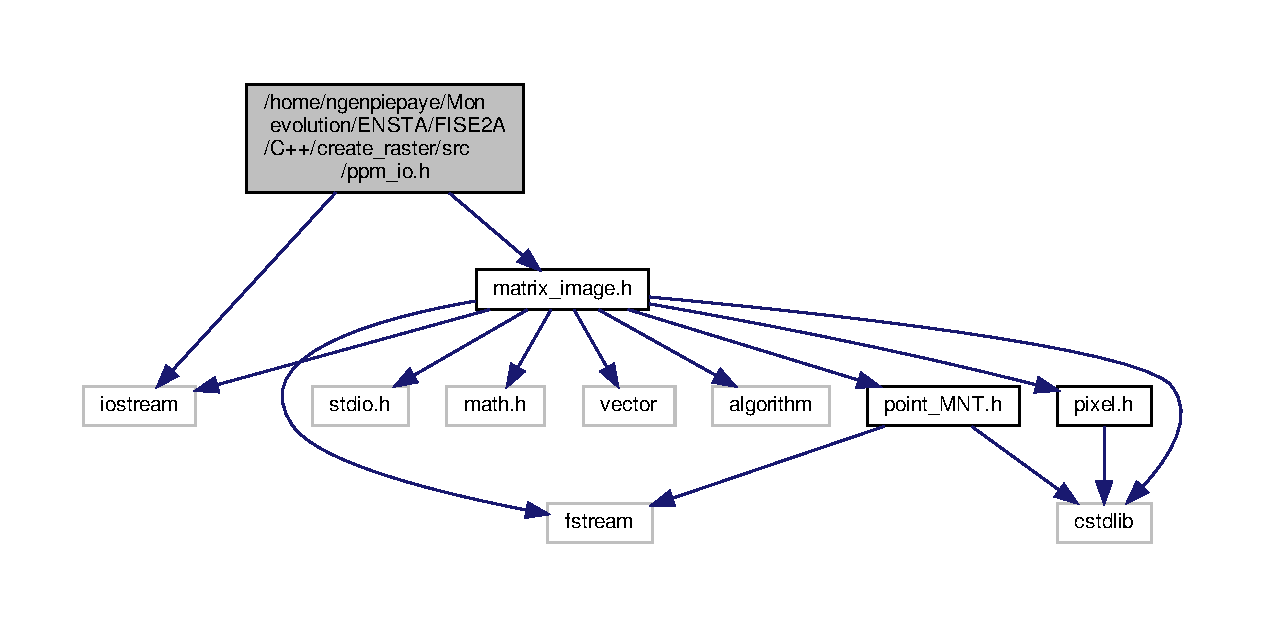
\includegraphics[width=350pt]{ppm__io_8h__incl}
\end{center}
\end{figure}
This graph shows which files directly or indirectly include this file\+:\nopagebreak
\begin{figure}[H]
\begin{center}
\leavevmode
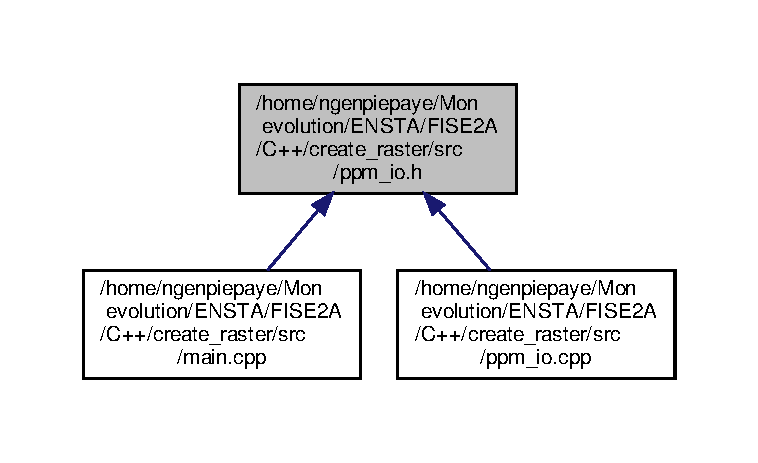
\includegraphics[width=350pt]{ppm__io_8h__dep__incl}
\end{center}
\end{figure}
\subsection*{Functions}
\begin{DoxyCompactItemize}
\item 
void \hyperlink{ppm__io_8h_a1e3323cf73c056dcf2fba982449cee66}{ppma\+\_\+write} (const string file\+\_\+out\+\_\+name, const \hyperlink{struct_matrix__image}{Matrix\+\_\+image} \&matrix)
\item 
void \hyperlink{ppm__io_8h_a93c152229441b701397eba28d74a081a}{ppma\+\_\+write\+\_\+data} (ofstream \&file\+\_\+out, const \hyperlink{struct_matrix__image}{Matrix\+\_\+image} \&matrix)
\item 
void \hyperlink{ppm__io_8h_a6b2d5a62a2152b60d2804a117f8f81b3}{ppma\+\_\+write\+\_\+header} (ofstream \&file\+\_\+out, const string file\+\_\+out\+\_\+name, const \hyperlink{struct_matrix__image}{Matrix\+\_\+image} \&matrix, const unsigned int maxg)
\item 
void \hyperlink{ppm__io_8h_a970ee41acf48504827a8fe77f0c29ffc}{ppmb\+\_\+write} (const string file\+\_\+out\+\_\+name, const \hyperlink{struct_matrix__image}{Matrix\+\_\+image} \&matrix)
\item 
void \hyperlink{ppm__io_8h_a15fab79ac0c0f8b7619665e591d75248}{ppmb\+\_\+write\+\_\+data} (ofstream \&file\+\_\+out, const \hyperlink{struct_matrix__image}{Matrix\+\_\+image} \&matrix)
\item 
void \hyperlink{ppm__io_8h_a7a5c7463f4f82aba6f68a99e7a343160}{ppmb\+\_\+write\+\_\+header} (ofstream \&file\+\_\+out, const string file\+\_\+out\+\_\+name, const \hyperlink{struct_matrix__image}{Matrix\+\_\+image} \&matrix, const unsigned int maxg)
\end{DoxyCompactItemize}


\subsection{Function Documentation}
\mbox{\Hypertarget{ppm__io_8h_a1e3323cf73c056dcf2fba982449cee66}\label{ppm__io_8h_a1e3323cf73c056dcf2fba982449cee66}} 
\index{ppm\+\_\+io.\+h@{ppm\+\_\+io.\+h}!ppma\+\_\+write@{ppma\+\_\+write}}
\index{ppma\+\_\+write@{ppma\+\_\+write}!ppm\+\_\+io.\+h@{ppm\+\_\+io.\+h}}
\subsubsection{\texorpdfstring{ppma\+\_\+write()}{ppma\_write()}}
{\footnotesize\ttfamily void ppma\+\_\+write (\begin{DoxyParamCaption}\item[{const string}]{output\+\_\+name,  }\item[{const \hyperlink{struct_matrix__image}{Matrix\+\_\+image} \&}]{matrix }\end{DoxyParamCaption})}

~\newline
$\ast$$\ast$$\ast$$\ast$$\ast$$\ast$$\ast$$\ast$$\ast$$\ast$$\ast$$\ast$$\ast$$\ast$$\ast$$\ast$$\ast$$\ast$$\ast$$\ast$$\ast$$\ast$$\ast$$\ast$$\ast$$\ast$$\ast$$\ast$$\ast$$\ast$$\ast$$\ast$$\ast$$\ast$$\ast$$\ast$$\ast$$\ast$$\ast$$\ast$$\ast$$\ast$$\ast$$\ast$$\ast$$\ast$$\ast$$\ast$$\ast$$\ast$$\ast$$\ast$$\ast$$\ast$$\ast$$\ast$$\ast$$\ast$$\ast$$\ast$$\ast$$\ast$$\ast$$\ast$$\ast$$\ast$$\ast$$\ast$$\ast$$\ast$$\ast$$\ast$$\ast$$\ast$$\ast$$\ast$~\newline
\textbackslash{} ~\newline
\textbackslash{} Purpose\+:~\newline
\textbackslash{} ~\newline
\textbackslash{} P\+P\+M\+A\+\_\+\+W\+R\+I\+TE writes the header and data for an A\+S\+C\+II P\+PM file.~\newline
\textbackslash{} ~\newline
\textbackslash{} example~\newline
\textbackslash{} ~\newline
\textbackslash{} P3~\newline
\textbackslash{} \# Le P3 signifie que les couleurs sont en A\+S\+C\+II, et qu\textquotesingle{}elles sont en R\+GB.~\newline
\textbackslash{} \# Par 3 colonnes et 2 lignes \+:~\newline
\textbackslash{} 3 2~\newline
\textbackslash{} \# Ayant 255 pour valeur maximum \+:~\newline
\textbackslash{} 255~\newline
\textbackslash{} 255 0 0 ~\newline
\textbackslash{} 0 255 0 ~\newline
 \textbackslash{} 0 0 255~\newline
\textbackslash{} 255 255 0 ~\newline
\textbackslash{} 255 255 255 ~\newline
 \textbackslash{} 0 0 0~\newline
\textbackslash{} ~\newline
\textbackslash{} Author\+:~\newline
\textbackslash{} ~\newline
\textbackslash{} Stephane N\+G\+N\+E\+P\+I\+E\+P\+A\+YE W\+E\+M\+BE~\newline
\textbackslash{} ~\newline
\textbackslash{} Parameters\+:~\newline
\textbackslash{} ~\newline
\textbackslash{} Input, string O\+U\+T\+P\+U\+T\+\_\+\+N\+A\+ME, the name of the file.~\newline
\textbackslash{} ~\newline
\textbackslash{} Input, \hyperlink{struct_matrix__image}{Matrix\+\_\+image}\& matrix matrix of pixel.~\newline
\textbackslash{} ~\newline


Definition at line 12 of file ppm\+\_\+io.\+cpp.

\mbox{\Hypertarget{ppm__io_8h_a93c152229441b701397eba28d74a081a}\label{ppm__io_8h_a93c152229441b701397eba28d74a081a}} 
\index{ppm\+\_\+io.\+h@{ppm\+\_\+io.\+h}!ppma\+\_\+write\+\_\+data@{ppma\+\_\+write\+\_\+data}}
\index{ppma\+\_\+write\+\_\+data@{ppma\+\_\+write\+\_\+data}!ppm\+\_\+io.\+h@{ppm\+\_\+io.\+h}}
\subsubsection{\texorpdfstring{ppma\+\_\+write\+\_\+data()}{ppma\_write\_data()}}
{\footnotesize\ttfamily void ppma\+\_\+write\+\_\+data (\begin{DoxyParamCaption}\item[{ofstream \&}]{output,  }\item[{const \hyperlink{struct_matrix__image}{Matrix\+\_\+image} \&}]{matrix }\end{DoxyParamCaption})}

~\newline
$\ast$$\ast$$\ast$$\ast$$\ast$$\ast$$\ast$$\ast$$\ast$$\ast$$\ast$$\ast$$\ast$$\ast$$\ast$$\ast$$\ast$$\ast$$\ast$$\ast$$\ast$$\ast$$\ast$$\ast$$\ast$$\ast$$\ast$$\ast$$\ast$$\ast$$\ast$$\ast$$\ast$$\ast$$\ast$$\ast$$\ast$$\ast$$\ast$$\ast$$\ast$$\ast$$\ast$$\ast$$\ast$$\ast$$\ast$$\ast$$\ast$$\ast$$\ast$$\ast$$\ast$$\ast$$\ast$$\ast$$\ast$$\ast$$\ast$$\ast$$\ast$$\ast$$\ast$$\ast$$\ast$$\ast$$\ast$$\ast$$\ast$$\ast$$\ast$$\ast$$\ast$$\ast$$\ast$$\ast$~\newline
\textbackslash{} ~\newline
\textbackslash{} Purpose\+:~\newline
\textbackslash{} ~\newline
\textbackslash{} P\+P\+M\+A\+\_\+\+W\+R\+I\+T\+E\+\_\+\+D\+A\+TA writes the data for an A\+S\+C\+II P\+PM file.~\newline
\textbackslash{} ~\newline
\textbackslash{} Author\+:~\newline
\textbackslash{} ~\newline
\textbackslash{} Stephane N\+G\+N\+E\+P\+I\+E\+P\+A\+YE W\+E\+M\+BE~\newline
\textbackslash{} ~\newline
\textbackslash{} Parameters\+:~\newline
\textbackslash{} ~\newline
\textbackslash{} Input, ofstream \&O\+U\+T\+P\+UT, a pointer to the file.~\newline
\textbackslash{} ~\newline
\textbackslash{} Input, \hyperlink{struct_matrix__image}{Matrix\+\_\+image}\& matrix matrix of pixel.~\newline
\textbackslash{} ~\newline


Definition at line 98 of file ppm\+\_\+io.\+cpp.

\mbox{\Hypertarget{ppm__io_8h_a6b2d5a62a2152b60d2804a117f8f81b3}\label{ppm__io_8h_a6b2d5a62a2152b60d2804a117f8f81b3}} 
\index{ppm\+\_\+io.\+h@{ppm\+\_\+io.\+h}!ppma\+\_\+write\+\_\+header@{ppma\+\_\+write\+\_\+header}}
\index{ppma\+\_\+write\+\_\+header@{ppma\+\_\+write\+\_\+header}!ppm\+\_\+io.\+h@{ppm\+\_\+io.\+h}}
\subsubsection{\texorpdfstring{ppma\+\_\+write\+\_\+header()}{ppma\_write\_header()}}
{\footnotesize\ttfamily void ppma\+\_\+write\+\_\+header (\begin{DoxyParamCaption}\item[{ofstream \&}]{output,  }\item[{const string}]{output\+\_\+name,  }\item[{const \hyperlink{struct_matrix__image}{Matrix\+\_\+image} \&}]{matrix,  }\item[{const unsigned int}]{maxg }\end{DoxyParamCaption})}

~\newline
$\ast$$\ast$$\ast$$\ast$$\ast$$\ast$$\ast$$\ast$$\ast$$\ast$$\ast$$\ast$$\ast$$\ast$$\ast$$\ast$$\ast$$\ast$$\ast$$\ast$$\ast$$\ast$$\ast$$\ast$$\ast$$\ast$$\ast$$\ast$$\ast$$\ast$$\ast$$\ast$$\ast$$\ast$$\ast$$\ast$$\ast$$\ast$$\ast$$\ast$$\ast$$\ast$$\ast$$\ast$$\ast$$\ast$$\ast$$\ast$$\ast$$\ast$$\ast$$\ast$$\ast$$\ast$$\ast$$\ast$$\ast$$\ast$$\ast$$\ast$$\ast$$\ast$$\ast$$\ast$$\ast$$\ast$$\ast$$\ast$$\ast$$\ast$$\ast$$\ast$$\ast$$\ast$$\ast$$\ast$~\newline
\textbackslash{} ~\newline
\textbackslash{} Purpose\+:~\newline
\textbackslash{} ~\newline
\textbackslash{} P\+P\+M\+A\+\_\+\+W\+R\+I\+T\+E\+\_\+\+H\+E\+A\+D\+ER writes the header of an A\+S\+C\+II P\+PM file.~\newline
\textbackslash{} ~\newline
\textbackslash{} Author\+:~\newline
\textbackslash{} ~\newline
\textbackslash{} Stephane N\+G\+N\+E\+P\+I\+E\+P\+A\+YE W\+E\+M\+BE~\newline
\textbackslash{} ~\newline
\textbackslash{} Parameters\+:~\newline
\textbackslash{} ~\newline
\textbackslash{} Input, ofstream \&O\+U\+T\+P\+UT, a pointer to the file.~\newline
\textbackslash{} ~\newline
\textbackslash{} Input, string O\+U\+T\+P\+U\+T\+\_\+\+N\+A\+ME, the name of the file.~\newline
\textbackslash{} ~\newline
\textbackslash{} Input, \hyperlink{struct_matrix__image}{Matrix\+\_\+image}\& matrix matrix of pixel.~\newline
\textbackslash{} ~\newline
\textbackslash{} Input, unsigned int M\+A\+XG, the maximum gray value.~\newline
\textbackslash{} ~\newline


Definition at line 140 of file ppm\+\_\+io.\+cpp.

\mbox{\Hypertarget{ppm__io_8h_a970ee41acf48504827a8fe77f0c29ffc}\label{ppm__io_8h_a970ee41acf48504827a8fe77f0c29ffc}} 
\index{ppm\+\_\+io.\+h@{ppm\+\_\+io.\+h}!ppmb\+\_\+write@{ppmb\+\_\+write}}
\index{ppmb\+\_\+write@{ppmb\+\_\+write}!ppm\+\_\+io.\+h@{ppm\+\_\+io.\+h}}
\subsubsection{\texorpdfstring{ppmb\+\_\+write()}{ppmb\_write()}}
{\footnotesize\ttfamily void ppmb\+\_\+write (\begin{DoxyParamCaption}\item[{string}]{output\+\_\+name,  }\item[{const \hyperlink{struct_matrix__image}{Matrix\+\_\+image} \&}]{matrix }\end{DoxyParamCaption})}

~\newline
$\ast$$\ast$$\ast$$\ast$$\ast$$\ast$$\ast$$\ast$$\ast$$\ast$$\ast$$\ast$$\ast$$\ast$$\ast$$\ast$$\ast$$\ast$$\ast$$\ast$$\ast$$\ast$$\ast$$\ast$$\ast$$\ast$$\ast$$\ast$$\ast$$\ast$$\ast$$\ast$$\ast$$\ast$$\ast$$\ast$$\ast$$\ast$$\ast$$\ast$$\ast$$\ast$$\ast$$\ast$$\ast$$\ast$$\ast$$\ast$$\ast$$\ast$$\ast$$\ast$$\ast$$\ast$$\ast$$\ast$$\ast$$\ast$$\ast$$\ast$$\ast$$\ast$$\ast$$\ast$$\ast$$\ast$$\ast$$\ast$$\ast$$\ast$$\ast$$\ast$$\ast$$\ast$$\ast$$\ast$ ~\newline
\textbackslash{} ~\newline
\textbackslash{} Purpose\+: ~\newline
\textbackslash{} ~\newline
\textbackslash{} P\+P\+M\+B\+\_\+\+W\+R\+I\+TE writes the header and data for a binary P\+PM file. ~\newline
\textbackslash{} ~\newline
\textbackslash{} example ~\newline
\textbackslash{} ~\newline
\textbackslash{} P3 ~\newline
\textbackslash{} \# Le P3 signifie que les couleurs sont en A\+S\+C\+II, et qu\textquotesingle{}elles sont en R\+GB. ~\newline
\textbackslash{} \# Par 3 colonnes et 2 lignes \+: ~\newline
\textbackslash{} 3 2 ~\newline
\textbackslash{} \# Ayant 255 pour valeur maximum \+: ~\newline
\textbackslash{} data ... ~\newline
\textbackslash{} ~\newline
\textbackslash{} Author\+:~\newline
\textbackslash{} ~\newline
\textbackslash{} Stephane N\+G\+N\+E\+P\+I\+E\+P\+A\+YE W\+E\+M\+BE ~\newline
\textbackslash{} ~\newline
\textbackslash{} Parameters\+: ~\newline
\textbackslash{} ~\newline
\textbackslash{} Input, string O\+U\+T\+P\+U\+T\+\_\+\+N\+A\+ME, the name of the file. ~\newline
\textbackslash{} ~\newline
 \textbackslash{} Input, \hyperlink{struct_matrix__image}{Matrix\+\_\+image}\& matrix matrix of pixel. ~\newline
\textbackslash{} ~\newline


Definition at line 175 of file ppm\+\_\+io.\+cpp.

\mbox{\Hypertarget{ppm__io_8h_a15fab79ac0c0f8b7619665e591d75248}\label{ppm__io_8h_a15fab79ac0c0f8b7619665e591d75248}} 
\index{ppm\+\_\+io.\+h@{ppm\+\_\+io.\+h}!ppmb\+\_\+write\+\_\+data@{ppmb\+\_\+write\+\_\+data}}
\index{ppmb\+\_\+write\+\_\+data@{ppmb\+\_\+write\+\_\+data}!ppm\+\_\+io.\+h@{ppm\+\_\+io.\+h}}
\subsubsection{\texorpdfstring{ppmb\+\_\+write\+\_\+data()}{ppmb\_write\_data()}}
{\footnotesize\ttfamily void ppmb\+\_\+write\+\_\+data (\begin{DoxyParamCaption}\item[{ofstream \&}]{output,  }\item[{const \hyperlink{struct_matrix__image}{Matrix\+\_\+image} \&}]{matrix }\end{DoxyParamCaption})}

~\newline
$\ast$$\ast$$\ast$$\ast$$\ast$$\ast$$\ast$$\ast$$\ast$$\ast$$\ast$$\ast$$\ast$$\ast$$\ast$$\ast$$\ast$$\ast$$\ast$$\ast$$\ast$$\ast$$\ast$$\ast$$\ast$$\ast$$\ast$$\ast$$\ast$$\ast$$\ast$$\ast$$\ast$$\ast$$\ast$$\ast$$\ast$$\ast$$\ast$$\ast$$\ast$$\ast$$\ast$$\ast$$\ast$$\ast$$\ast$$\ast$$\ast$$\ast$$\ast$$\ast$$\ast$$\ast$$\ast$$\ast$$\ast$$\ast$$\ast$$\ast$$\ast$$\ast$$\ast$$\ast$$\ast$$\ast$$\ast$$\ast$$\ast$$\ast$$\ast$$\ast$$\ast$$\ast$$\ast$$\ast$ ~\newline
\textbackslash{} ~\newline
\textbackslash{} Purpose\+: ~\newline
\textbackslash{} ~\newline
\textbackslash{} P\+P\+M\+B\+\_\+\+W\+R\+I\+T\+E\+\_\+\+D\+A\+TA writes the data for a binary P\+PM file. ~\newline
\textbackslash{} ~\newline
\textbackslash{} Author\+: ~\newline
\textbackslash{} ~\newline
\textbackslash{} Stephane N\+G\+N\+E\+P\+I\+E\+P\+A\+YE W\+E\+M\+BE ~\newline
\textbackslash{} ~\newline
\textbackslash{} Parameters\+: ~\newline
\textbackslash{} ~\newline
\textbackslash{} Input, ofstream \&O\+U\+T\+P\+UT, a pointer to the file.~\newline
\textbackslash{} ~\newline
\textbackslash{} Input, \hyperlink{struct_matrix__image}{Matrix\+\_\+image}\& matrix matrix of pixel. ~\newline
 \textbackslash{} ~\newline
 

Definition at line 254 of file ppm\+\_\+io.\+cpp.

\mbox{\Hypertarget{ppm__io_8h_a7a5c7463f4f82aba6f68a99e7a343160}\label{ppm__io_8h_a7a5c7463f4f82aba6f68a99e7a343160}} 
\index{ppm\+\_\+io.\+h@{ppm\+\_\+io.\+h}!ppmb\+\_\+write\+\_\+header@{ppmb\+\_\+write\+\_\+header}}
\index{ppmb\+\_\+write\+\_\+header@{ppmb\+\_\+write\+\_\+header}!ppm\+\_\+io.\+h@{ppm\+\_\+io.\+h}}
\subsubsection{\texorpdfstring{ppmb\+\_\+write\+\_\+header()}{ppmb\_write\_header()}}
{\footnotesize\ttfamily void ppmb\+\_\+write\+\_\+header (\begin{DoxyParamCaption}\item[{ofstream \&}]{output,  }\item[{const string}]{output\+\_\+name,  }\item[{const \hyperlink{struct_matrix__image}{Matrix\+\_\+image} \&}]{matrix,  }\item[{const unsigned int}]{maxg }\end{DoxyParamCaption})}

~\newline
$\ast$$\ast$$\ast$$\ast$$\ast$$\ast$$\ast$$\ast$$\ast$$\ast$$\ast$$\ast$$\ast$$\ast$$\ast$$\ast$$\ast$$\ast$$\ast$$\ast$$\ast$$\ast$$\ast$$\ast$$\ast$$\ast$$\ast$$\ast$$\ast$$\ast$$\ast$$\ast$$\ast$$\ast$$\ast$$\ast$$\ast$$\ast$$\ast$$\ast$$\ast$$\ast$$\ast$$\ast$$\ast$$\ast$$\ast$$\ast$$\ast$$\ast$$\ast$$\ast$$\ast$$\ast$$\ast$$\ast$$\ast$$\ast$$\ast$$\ast$$\ast$$\ast$$\ast$$\ast$$\ast$$\ast$$\ast$$\ast$$\ast$$\ast$$\ast$$\ast$$\ast$$\ast$$\ast$$\ast$ ~\newline
\textbackslash{} ~\newline
\textbackslash{} Purpose\+: ~\newline
\textbackslash{} ~\newline
\textbackslash{} P\+P\+M\+B\+\_\+\+W\+R\+I\+T\+E\+\_\+\+H\+E\+A\+D\+ER writes the header of a binary P\+PM file. ~\newline
\textbackslash{} ~\newline
\textbackslash{} Author\+: ~\newline
\textbackslash{} ~\newline
\textbackslash{} Stephane N\+G\+N\+E\+P\+I\+E\+P\+A\+YE W\+E\+M\+BE ~\newline
\textbackslash{} ~\newline
\textbackslash{} Parameters\+:~\newline
\textbackslash{} ~\newline
\textbackslash{} Input, ofstream \&O\+U\+T\+P\+UT, a pointer to the file. ~\newline
\textbackslash{} ~\newline
\textbackslash{} Input, string O\+U\+T\+P\+U\+T\+\_\+\+N\+A\+ME, the name of the file.~\newline
\textbackslash{} ~\newline
\textbackslash{} Input, \hyperlink{struct_matrix__image}{Matrix\+\_\+image}\& matrix matrix of pixel. ~\newline
\textbackslash{} ~\newline
\textbackslash{} Input, unsigned int M\+A\+XG, the maximum gray value. ~\newline
\textbackslash{} ~\newline


Definition at line 291 of file ppm\+\_\+io.\+cpp.


%--- End generated contents ---

% Index
\backmatter
\newpage
\phantomsection
\clearemptydoublepage
\addcontentsline{toc}{chapter}{Index}
\printindex

\end{document}
